%%%%%%%%%%%%%%%%%%%%%%%%%%%%%%%%%%%%%%%%%%%%%%%%%%%%%%%%%%%%%%%
%% OXFORD THESIS TEMPLATE

% Use this template to produce a standard thesis that meets the Oxford University requirements for DPhil submission
%
% Originally by Keith A. Gillow (gillow@maths.ox.ac.uk), 1997
% Modified by Sam Evans (sam@samuelevansresearch.org), 2007
% Modified by John McManigle (john@oxfordechoes.com), 2015
%
% This version Copyright (c) 2015-2017 John McManigle
%
% Broad permissions are granted to use, modify, and distribute this software
% as specified in the MIT License included in this distribution's LICENSE file.
%

% I've (John) tried to comment this file extensively, so read through it to see how to use the various options.  Remember
% that in LaTeX, any line starting with a % is NOT executed.  Several places below, you have a choice of which line to usehttps://www.overleaf.com/project/608c260a6b68867d04f5d4c2
% out of multiple options (eg draft vs final, for PDF vs for binding, etc.)  When you pick one, add a % to the beginning of
% the lines you don't want.

%%%%% CHOOSE PAGE LAYOUT
% The most common choices should be below.  You can also do other things, like replacing "a4paper" with "letterpaper", etc.

% This one will format for two-sided binding (ie left and right pages have mirror margins; blank pages inserted where needed):
%\documentclass[a4paper,twoside]{ociamthesis}
% This one will format for one-sided binding (ie left margin > right margin; no extra blank pages):
%\documentclass[a4paper]{ociamthesis}
% This one will format for PDF output (ie equal margins, no extra blank pages):
\documentclass[a4paper,nobind]{ociamthesis} 



%%%%% SELECT YOUR DRAFT OPTIONS
% Three options going on here; use in any combination.  But remember to turn the first two off before
% generating a PDF to send to the printer!

% This adds a "DRAFT" footer to every normal page.  (The first page of each chapter is not a "normal" page.)
\fancyfoot[C]{\emph{DRAFT Printed on \today}}  

% This highlights (in blue) corrections marked with (for words) \mccorrect{blah} or (for whole
% paragraphs) \begin{mccorrection} . . . \end{mccorrection}.  This can be useful for sending a PDF of
% your corrected thesis to your examiners for review.  Turn https://www.overleaf.com/project/608c260a6b68867d04f5d4c2it off, and the blue disappears.
\correctionstrue


% The science-type option: numerical in-text citation with references in order of appearance.
\usepackage[style=numeric-comp, sorting=none, backend=biber, doi=false, isbn=false]{biblatex}
\newcommand*{\bibtitle}{References}

% The humanities-type option: author-year in-text citation with an alphabetical works cited.
%\usepackage[style=authoryear, sorting=nyt, backend=biber, maxcitenames=2, useprefix, doi=false, isbn=false]{biblatex}
%\newcommand*{\bibtitle}{Works Cited}

% This makes the bibliography left-aligned (not 'justified') and slightly smaller font.
\renewcommand*{\bibfont}{\raggedright\small}

% Change this to the name of your .bib file (usually exported from a citation manager like Zotero or EndNote).
\addbibresource{references.bib}

\usepackage{algorithmic}
\usepackage{amssymb}
\usepackage{amsmath}

\usepackage{tabularx} % extra features for tabular environmentw
\usepackage{graphicx} % takes care of graphic including machinery
\usepackage{subcaption}
\usepackage{blindtext}
\usepackage[export]{adjustbox}
\usepackage{graphicx}% http://ctan.org/pkg/graphicx
\usepackage{listings}

\usepackage{fancyvrb}

% redefine \VerbatimInput
\RecustomVerbatimCommand{\VerbatimInput}{VerbatimInput}%
{fontsize=\footnotesize,
 %
 frame=lines,  % top and bottom rule only
 framesep=2em, % separation between frame and text
 %
 %
 commandchars=\|\(\), % escape character and argument delimiters for
                      % commands within the verbatim
}

% Uncomment this if you want equation numbers per section (2.3.12), instead of per chapter (2.18):
%\numberwithin{equation}{subsection}



%%%%% THESIS / TITLE PAGE INFORMATION
% Everybody needs to complete the following:
\title{Advanced Analysis Methods for Imaging Atmospheric Cherenkov Telescope Data with SSTCAM and VERITAS}
\author{Samuel Timothy Spencer}
\college{Exeter College}

% Master's candidates who require the alternate title page (with candidate number and word count)
% must also un-comment and complete the following three lines:
%\masterssubmissiontrue
%\candidateno{933516}
%\wordcount{28,815}

% Uncomment the following line if your degree also includes exams (eg most masters):
%\renewcommand{\submittedtext}{Submitted in partial completion of the}
% Your full degree name.  (But remember that DPhils aren't "in" anything.  They're just DPhils.)
\degree{Doctor of Philosophy}
% Term and year of submission, or date if your board requires (eg most masters)
\degreedate{Trinity 2021}


%%%%% YOUR OWN PERSONAL MACROS
% This is a good place to dump your own LaTeX macros as they come up.

% To make text superscripts shortcuts
	\renewcommand{\th}{\textsuperscript{th}} % ex: I won 4\th place
	\newcommand{\nd}{\textsuperscript{nd}}
	\renewcommand{\st}{\textsuperscript{st}}
	\newcommand{\rd}{\textsuperscript{rd}}

%%%%% THE ACTUAL DOCUMENT STARTS HERE
\begin{document}



%%%%% CHOOSE YOUR LINE SPACING HERE
% This is the official option.  Use it for your submission copy and library copy:
\setlength{\textbaselineskip}{22pt plus2pt}
% This is closer spacing (about 1.5-spaced) that you might prefer for your personal copies:
%\setlength{\textbaselineskip}{18pt plus2pt minus1pt}

% You can set the spacing here for the roman-numbered pages (acknowledgements, table of contents, etc.)
\setlength{\frontmatterbaselineskip}{17pt plus1pt minus1pt}

% Leave this line alone; it gets things started for the real document.
\setlength{\baselineskip}{\textbaselineskip}


%%%%% CHOOSE YOUR SECTION NUMBERING DEPTH HERE
% You have two choices.  First, how far down are sections numbered?  (Below that, they're named but
% don't get numbers.)  Second, what level of section appears in the table of contents?  These don't have
% to match: you can have numbered sections that don't show up in the ToC, or unnumbered sections that
% do.  Throughout, 0 = chapter; 1 = section; 2 = subsection; 3 = subsubsection, 4 = paragraph...

% The level that gets a number:
\setcounter{secnumdepth}{2}
% The level that shows up in the ToC:
\setcounter{tocdepth}{2}


%%%%% ABSTRACT SEPARATE
% This is used to create the separate, one-page abstract that you are required to hand into the Exam
% Schools.  You can comment it out to generate a PDF for printing or whatnot.
\begin{abstractseparate}
	Your abstract text goes here.  Check your departmental regulations, but generally this should be less than 300 words.
 % Create an abstract.tex file in the 'text' folder for your abstract.
\end{abstractseparate}


% JEM: Pages are roman numbered from here, though page numbers are invisible until ToC.  This is in
% keeping with most typesetting conventions.
\begin{romanpages}

% Title page is created here
\maketitle

%%%%% DEDICATION -- If you'd like one, un-comment the following.
%\begin{dedication}
%This thesis is dedicated to\\
%someone\\
%for some special reason\\
%\end{dedication}

%%%%% ACKNOWLEDGEMENTS -- Nothing to do here except comment out if you don't want it.
\begin{acknowledgements}
 	\subsection*{Personal}

This is where you thank your advisor, colleagues, and family and friends.

Figures are my own, unless expressly stated otherwise. 

T. Armstrong performed simulations needed for the results in Chapter \ref{ch:3-TimingInfo}, though the analysis of those simulations was performed by myself. R. Prado played a similar role for the simulations used in \ref{ch:4-VERITASRealData}, and G. Maier made the changes needed to \textit{eventdisplay} that made the deep learning analysis possible, although I was responsible for the creation of the rest of the analysis pipeline.


\subsection*{Institutional}

Chapter 3: This work used the European Grid Infrastructure. We thank Luisa Arrabito and Johan Bregeon for their assistance in running our simulations and code on it. Later training runs in this paper used the \textit{Glamdring} cluster in Oxford; we thank Jonathan Patterson for his work in upgrading and maintaining this facility. SS acknowledges an STFC Ph.D. studentship. GC, JW and TA acknowledge support from STFC grants ST/S002618/1 and ST/M00757X/1. GC acknowledges support from Exeter College, Oxford. This work has gone through internal review by the CTA Consortium, who we thank for allowing us to use CTA simulation models. We gratefully acknowledge financial support from the agencies and organisations listed here: \url{http://www.cta-observatory.org/consortium\_acknowledgments}.
\end{acknowledgements}
\begin{originality}
 	The material in this thesis has not been submitted for examination at the University of Oxford or at any other university. All the work within this thesis is my own, along with all figures (unless explicitly stated otherwise). Work from this thesis has been published in the following works (of which I was first author):

\begin{centering}
\begin{itemize}
    \item S. Spencer et al., Prospects for the Use of Photosensor Timing Information with Machine Learning Techniques in Background Rejection, PoS(ICRC2019) 798 (2019).
    \item S. Spencer et al., Deep Learning with Photosensor Timing Information as a Background Rejection Method for the Cherenkov Telescope Array, Astroparticle Physics 129C 102579 (2021).
    \item S. Spencer et al., Advanced Studies of SSTCAM Night Sky Background, Spencer et al., SSTCAM Internal Note (2021). 
\end{itemize}
\end{centering}

Chapters 3 and 5 detail work that was performed in the context of the CHEC (later SSTCAM) collaborations, and also the wider Analysis and Simulations Working Group (ASWG) of CTA. Chapter 4 contains work performed in collaboration with the VERITAS collaboration.

T. Armstrong performed simulations needed for the results in Chapter \ref{ch:3-TimingInfo}, though the analysis of those simulations was performed by myself. R. Prado played a similar role for the simulations used in Chapter \ref{ch:4-VERITASRealData}, and G. Maier made the changes needed to \textit{Eventdisplay} to make it compatible with the deep learning analysis, although I was responsible for the creation of the rest of the analysis pipeline.
\end{originality}
%%%%% ABSTRACT -- Nothing to do here except comment out if you don't want it.
\begin{abstract}
	Your abstract text goes here.  Check your departmental regulations, but generally this should be less than 300 words.

\end{abstract}

%%%%% MINI TABLES
% This lays the groundwork for per-chapter, mini tables of contents.  Comment the following line
% (and remove \minitoc from the chapter files) if you don't want this.  Un-comment either of the
% next two lines if you want a per-chapter list of figures or tables.
\dominitoc % include a mini table of contents
%\dominilof  % include a mini list of figures
%\dominilot  % include a mini list of tables

% This aligns the bottom of the text of each page.  It generally makes things look better.
\flushbottom

% This is where the whole-document ToC appears:
\tableofcontents

\listoffigures
	\mtcaddchapter
% \mtcaddchapter is needed when adding a non-chapter (but chapter-like) entity to avoid confusing minitoc

% Uncomment to generate a list of tables:
%\listoftables
%	\mtcaddchapter

%%%%% LIST OF ABBREVIATIONS
% This example includes a list of abbreviations.  Look at text/abbreviations.tex to see how that file is
% formatted.  The template can handle any kind of list though, so this might be a good place for a
% glossary, etc.
% First parameter can be changed eg to "Glossary" or something.
% Second parameter is the max length of bold terms.
\begin{mclistof}{List of Abbreviations}{3.2cm}

\item[1D, 2D, 3D] One, two or three dimensional, referring in this thesis to spatial dimensions in an image.

\item[CHEC] The Compact High Energy Camera, a class of prototype.
\item[CNN] Convolutional Neural Network, a form of machine learning algorithm designed to work with images.
\item[CTA] Cherenkov Telescope Array, the planned successor to the current generation of IACTs.
\item{DL} Deep Learning. Refers to machine learning with a high degree of depth (or equivalently abstraction of learned features).
\item[IACT]Imaging Atmospheric Cherenkov Telescope.
\item[LST] Large Size Telescope; the largest CTA telescope class designed to operate at the lowest energies.
\item[ML] Machine Learning
\item[MST] The Medium Size Telescope; the intermediate size CTA telescope class.
\item[NSB] Night Sky Background to IACTs
\item[SCT] The Swartzchild Couder Telescope; an alternative, American lead dual mirror prototype design for the MST.
\item[SST] Small Size Telescope; the smallest CTA telescope designed to operate at the highest energies.

\end{mclistof} 

% The Roman pages, like the Roman Empire, must come to its inevitable close.
\end{romanpages}


%%%%% CHAPTERS
% Add or remove any chapters you'd like here, by file name (excluding '.tex'):
\flushbottom
\chapter{\label{ch:1-intro}Introduction} 
\minitoc
\section{Astrophysics in the \ensuremath{\gamma}-Ray Domain}
$\gamma$-rays are generally considered to be photons with energies in excess of 100 keV, though there is no strict cutoff against X-rays. A wide variety of astrophysical objects produce $\gamma$-rays, including Supernova Remnants (SNR), Activate Galactic Nuclei (AGN) and pulsars (to name but a few) \cite{scienceCTA}. In order to fully understand these objects, we need to capture maximal information about their emission across the entire electromagnetic spectrum, as well as with multi-messenger methods (neutrinos, gravitational waves and cosmic rays).  Performing electromagnetic observations of these sources at high photon energies is challenging for a number of reasons \cite{jamieiact}. Firstly, these $\gamma$-rays cannot be focused and as such it is necessary to use particle physics techniques to reconstruct their point of origin. Secondly, $\gamma$-rays do not penetrate the Earth's atmosphere, meaning that in order to detect $\gamma$-rays directly the instrument must be in space. Finally, $\gamma$-rays are comparatively rare (the brightest astrophysical $\gamma$-ray sources have a flux of about 6 $\rm{photons} \ \rm{m}^{-2}\ \rm{year}^{-1}$ above 1TeV\cite{jamieiact}), meaning that in order to detect the highest energy $\gamma$-rays one must use an instrument with a very large effective area.
\section{Direct \ensuremath{\gamma}-ray Detection}
\subsection{Early Missions}
The problems in observing astrophysical $\gamma$-rays related to Earth's atmosphere can be solved by observing in space. Following theoretical predictions of cosmic $\gamma$-ray emission in the 1940s and 1950s \cite{morrison}, the first instrument to directly observe astrophysical $\gamma$-rays was \textit{Explorer} 11. Launched on 17th November 1961 \cite{explorer}, it consisted of two instruments. Firstly, its Phoswich-Cherenkov Counter Telescope consisted of a sandwich of NaI and CsI scintillator viewed by a single photomultiplier. Secondly, \textit{Explorer} 11 had a  Lucite Cherenkov counter viewed by two photomultipliers. Explorer 11 detected 22 $\gamma$-rays from all directions, suggesting the existence of a $\gamma$-ray background, but no point sources were seen in the data. The later, \textit{OSO} 3 mission (which was similar but with improved energy resolution) was able to separate this diffuse emission into galactic and extragalactic components \cite{oso3}. It wasn't until the \textit{SAS-2} \cite{sas2} and \textit{COS-B} \cite{cosb} missions (the latter of which used an innovative spark chamber system to track electrons and positrons from $\gamma$-ray pair production) in the 1970s that persistant $\gamma$-ray point sources, such as the pulsar Geminga, were observed.

Concurrently, the \textit{Vela} satellites were a series of American satellites launched to monitor the partial nuclear test ban treaty, the first of which was launched in 1963. On July 2, 1967 at 14:19, \textit{Vela} 3 and 4 observed a bright flash of $\gamma$-rays unlike any nuclear explosion observed before, seemingly originating from space \footnote{One would hope this alone was evidence enough of astrophysical $\gamma$-ray emission, however the USA had previously detonated a series of nuclear weapons in space, beginning with the 1.4 megaton \textit{Starfish Prime} test in 1962 \cite{starfish}.}. Due to \textit{Vela} results being classified, it wasn't until 1973 that this signal (along with 15 others) was published as evidence of astrophysical Gamma-Ray Bursts (GRBs), the most energetic astrophysical objects ever detected \cite{velagrb}. The first space-based telescope to simultaneously perform GRB monitoring and a survey of persistant $\gamma$-ray emitters was the Compton $\gamma$-ray observatory in the 1990s (billed as one of NASA's `great observatories' alongside the Hubble Space Telescope) \cite{compton}. The challenge of building instruments sensitive enough to observe persistant sources as well as rapid enough to observe GRBs continues to this day \cite{magicGRB}.

\subsection{The Fermi Space Telescope}
\begin{figure}[ht] 
        % read manual to see what [ht] means and for other possible options
        \centering 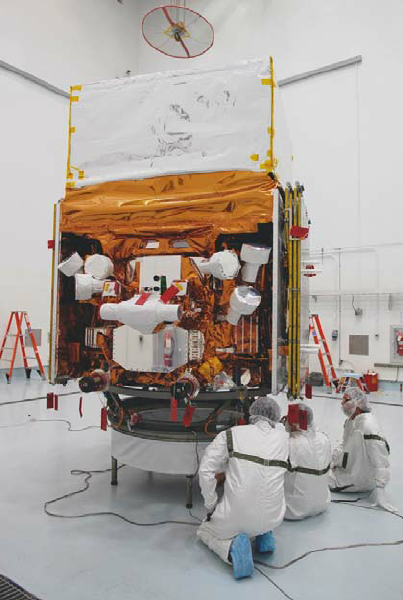
\includegraphics[width=0.5\columnwidth]{figures/fermi2.png}

        % note that in above figure file name, "sr_setup",
        % the file extension is missing. LaTeX is smart enough to find
        % apropriate one (i.e. pdf, png, etc.)
        % You can add this extention yourself as it seen below
        % both notations are correct but above has more flexibility
        %\includegraphics[width=1.0\columnwidth]{sr_setup.pdf}
        \caption{
                \label{fig:fermi} % spaces are big no-no withing labels
                % things like fig: are optional in the label but it helps
                % to orient yourself when you have multiple figures,
                % equations and tables
                The \textit{Fermi} space telescope on Earth, with its solar arrays folded. LAT is the block at the top of the satellite covered with the silver anti-coincidence shield. GBM consists of the cylindrical structures protruding from the lower half of the telescope. Note the size of the engineers relative to the size of the instrument, this highlights the comparatively small effective area of LAT. Image credit: NASA/Kim Shiflett.
        }
\end{figure}

The current workhorse for the majority of space-based $\gamma$-ray observations is the very successful \textit{Fermi} space telescope, which has operated since 2008. \textit{Fermi} is equipped with two instruments, the Large Area Telescope (LAT) which surveys the entire $\gamma$-ray sky every three hours, and the Gamma-Ray Burst Monitor (GBM), which is specifically designed to detect GRBs and solar flares. LAT consists of 18 layers of silicon strip detectors designed to promote pair production from incident $\gamma$-rays, and detect the resultant charged products, as well as a scintillator calorimeter to measure the resultant $\mathrm{e^+/e^-}$ energy (similar in concept to COS-B). LAT is able to achieve near perfect background rejection of charged cosmic rays due to the presence of a conducting anti-coincidence shield that surrounds the instrument, such that if a charge signal is detected the instrument will not trigger. GBM consists of two sets of detectors: twelve sodium iodide (NaI) scintillators, and two cylindrical bismuth germanate (BGO) scintillators, and through this can reconstruct the positions of GRBs anywhere on the sky not occluded by the Earth. 

Notable major discoveries by \textit{Fermi} include the detection of the Fermi bubbles, large $\gamma$-ray emitting structures extending to around $\mathrm{20^{\circ}}$ degrees above and below the galactic plane \cite{hooperslayter}, as well as the detection of the short GRB 170817 coincident with a gravitational wave event (GW170817) from a binary neutron star merger \cite{ligogrb}. However, the energy range of LAT is limited to between 20MeV and 300GeV because of the small effective area of the detector. As such, in order to observe higher energy photons (in the high GeV-TeV energy range) we must detect them indirectly. This can be performed using the Imaging Atmospheric Cherenkov Telescope  (IACT) method, pioneered by Jelly and Galbraith in 1953 \cite{G+J}, and by utilising water Cherenkov detectors  \cite{hawc}. Both of these operate by detecting the Extensive Air Shower (EAS) created when a high energy $\gamma$-ray interacts with Earth's atmosphere. We discuss the specifics of these detectors in the next section. 

\section{Indirect \ensuremath{\gamma}-ray Detection}
\subsection{The Cherenkov Effect}
Both IACTs and water Cherenkov detectors ultimately rely upon the Cherenkov effect. Cherenkov light is the light emitted by a medium when a charged particle passes through it at faster than the phase velocity of light. An image qualitatively describing the effect can be seen in Figure \ref{fig:jelley}. When a charged particle is at a point P in a dielectric, the atoms surrounding it behave like simple dipoles, with the positive end of the dipole reorienting to point towards the particle if the particle is negatively charged and vice versa. If the particle travels sufficiently slowly, the polarization field surrounding the particle will be completely symmetric, and so when the particle moves on to a new position P', there is no net electric field at far distance and so no emission. However, if the particle travels faster than the phase velocity of light, whilst the polarization field will still be symmetric along the axis of movement, it will no longer be symmetric in azimuth. This means that when the system relaxes as the particle moves on a light pulse will be generated \cite{jelley}. As such, as the particle travels through the medium, successive brief pulses of light are generated. 

\begin{figure}[ht] 
        % read manual to see what [ht] means and for other possible options
        \centering 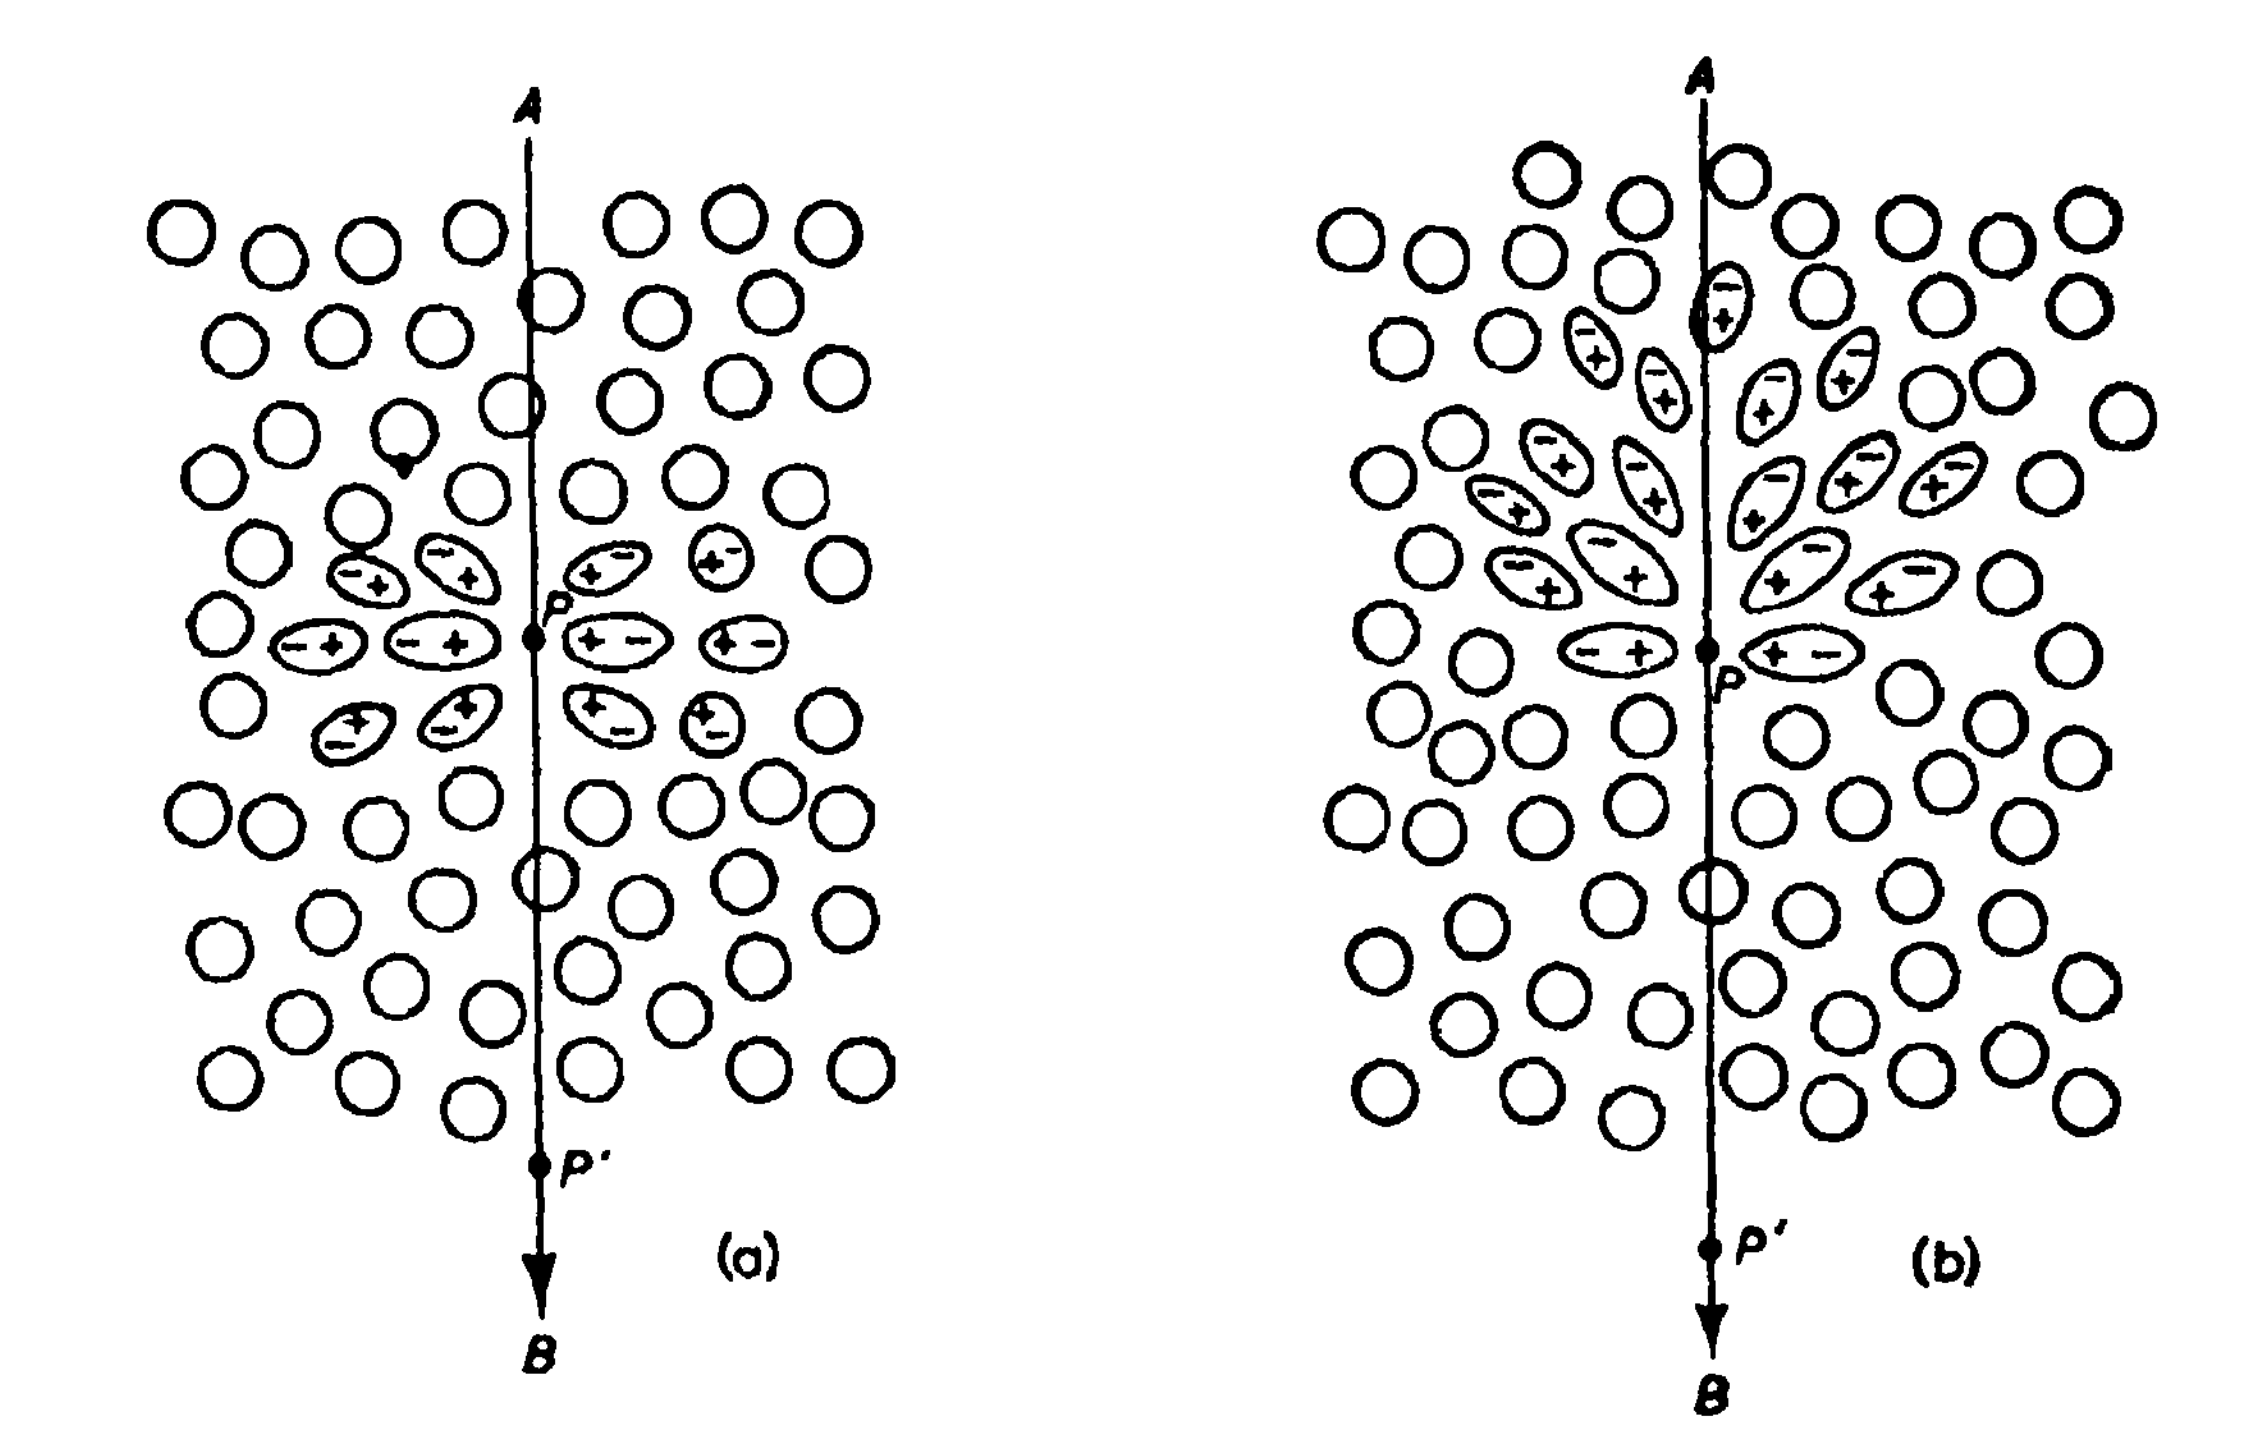
\includegraphics[width=0.7\columnwidth]{figures/dipole.png}

        % note that in above figure file name, "sr_setup",
        % the file extension is missing. LaTeX is smart enough to find
        % apropriate one (i.e. pdf, png, etc.)
        % You can add this extention yourself as it seen below
        % both notations are correct but above has more flexibility
        %\includegraphics[width=1.0\columnwidth]{sr_setup.pdf}
        \caption{
                \label{fig:jelley} % spaces are big no-no withing labels
                % things like fig: are optional in the label but it helps
                % to orient yourself when you have multiple figures,
                % equations and tables
                The polarization set up in a medium by the passage of a charged particle at low velocity (left,a) and high velocity (right,b). Figure taken from \cite{jelley}.
        }
\end{figure}
\begin{figure}[t] 
        % read manual to see what [ht] means and for other possible options
        \centering 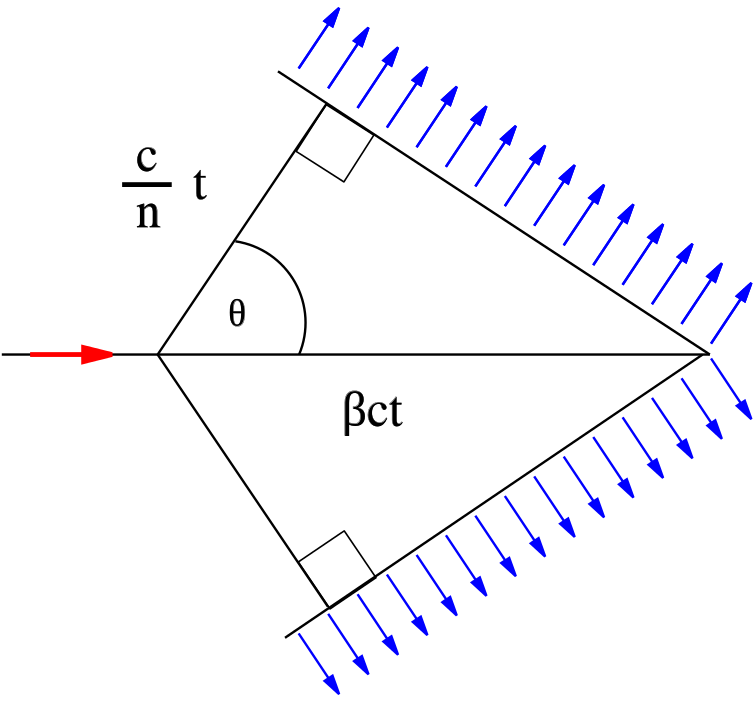
\includegraphics[width=0.5\columnwidth]{figures/Cherenkov.png}

        % note that in above figure file name, "sr_setup",
        % the file extension is missing. LaTeX is smart enough to find
        % apropriate one (i.e. pdf, png, etc.)
        % You can add this extention yourself as it seen below
        % both notations are correct but above has more flexibility
        %\includegraphics[width=1.0\columnwidth]{sr_setup.pdf}
        \caption{
                \label{fig:cherenkov} % spaces are big no-no withing labels
                % things like fig: are optional in the label but it helps
                % to orient yourself when you have multiple figures,
                % equations and tables
                The geometry of the Cherenkov effect, assuming no dispersion. Image credit: A. Horvarth.
        }
\end{figure}

As can be seen in Figure \ref{fig:cherenkov}, this results in the emitted light being distributed according to the Cherenkov opening angle $\theta_c$
\begin{equation}
    \cos\theta_c=\frac{1}{n\beta}
    \label{eq:cherenkov}
\end{equation}

where $n$ is the refractive index, $\beta$=$v/c$ where $v$ is the velocity of light in the medium and $c$ is the speed of light in a vacuum.

The energy $dE$ emitted as a result of the particle traversing the medium per unit length $dx$ is given by the Frank-Tamm formula, derived using the framework of special relativity in 1937 (and winning the authors a Nobel prize in 1958, along with Cherenkov). This holds provided the velocity $v$ as a fraction of the speed of light in a vacuum $c$ is greater than $\frac{1}{n(\omega)}$ (where $n(\omega)$ is the frequency dependent refractive index)
\begin{equation}
    \frac{d^2E}{dx\ d\omega}=\frac{q^2}{4\pi}\mu(\omega)\omega\left(1- \frac{c^2}{v^2(\omega)} \right)
    \label{eq:FT}
\end{equation}
where $\mu(\omega)$ is the frequency dependent permeability, and $q$ is the charge of the particle \cite{franktamm}. The total energy emitted in Cherenkov radiation is therefore given by the corresponding integral
\begin{equation}
    \frac{dE}{dx}=\frac{q^2}{4\pi}\int_{v>\frac{c}{n(\omega)}}^{\infty}\mu(\omega)\omega \left(1- \frac{c^2}{v^2n^2(\omega)} \right) d \omega .
    \label{eq:FT2}
\end{equation}

This integral is finite as $\lim_{\omega \to \infty} n(\omega)<1$ and $\lim_{\omega \to 0} n(\omega)=1$ . Assuming $\mu(v)$ is unity equation \ref{eq:FT} can also be integrated over frequency \cite{katz} to get the number of Cherenkov photons $dN_{\gamma}$ emitted per unit length
\begin{equation}
    \frac{dN_{\gamma}}{dx}=2\pi\alpha \left( 1- \frac{1}{\beta^2n^2} \right) \left(\frac{1}{\lambda_{min}}-\frac{1}{\lambda_{max}} \right)
\end{equation}
where $\alpha$ is the fine structure constant, and the $\lambda$ terms represent the minimum and maximum wavelength range of the emission. Taking this band to be 300nm-600nm and $\beta$=1 implies $\frac{dN_{\gamma}}{dx}$ is around $\mathrm{15 m^{-1}}$ at an 8km altitude in air \cite{katz}. 
\subsection{IACT Basics}

\begin{figure}[ht] 
        % read manual to see what [ht] means and for other possible options
        \centering 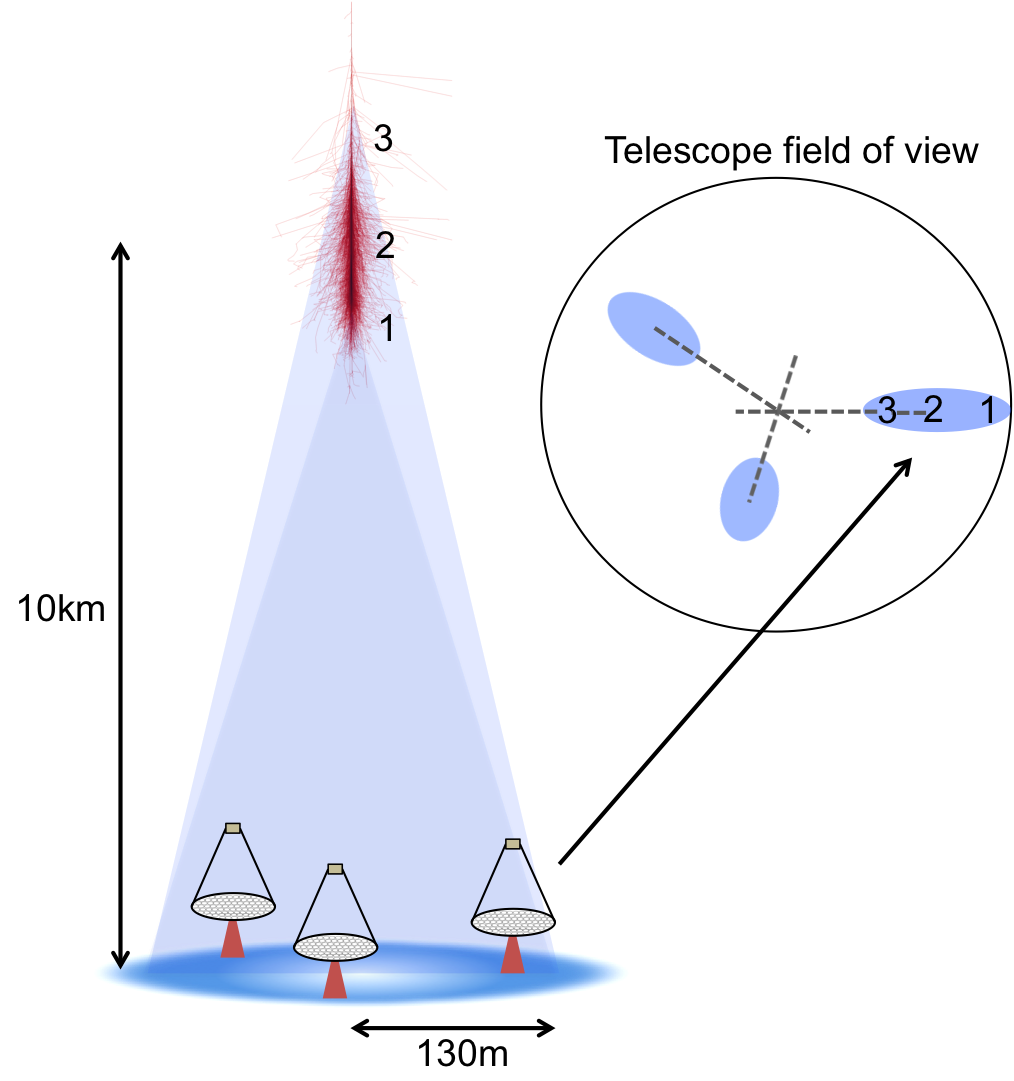
\includegraphics[width=0.7\columnwidth]{figures/schematic.png}

        % note that in above figure file name, "sr_setup",
        % the file extension is missing. LaTeX is smart enough to find
        % apropriate one (i.e. pdf, png, etc.)
        % You can add this extention yourself as it seen below
        % both notations are correct but above has more flexibility
        %\includegraphics[width=1.0\columnwidth]{sr_setup.pdf}
        \caption{
                \label{fig:schem} % spaces are big no-no withing labels
                % things like fig: are optional in the label but it helps
                % to orient yourself when you have multiple figures,
                % equations and tables
                A schematic of the IACT technique, taken from \cite{jamieiact}. Three telescopes stereoscopically observe a
                Cherenkov light pool caused by an EAS. The direction of the incident photon is reconstructed by intersecting the primary axes of 				 the elliptical images in the three cameras. On the right, an illustration that the light from the lowest altitude part of the shower is the first to arrive on the ground.
        }
\end{figure}
When a photon with an energy of above around 50GeV encounters the Earth's atmosphere, it undergoes pair production in the electric field of the nucleus of an atmospheric molecule $X$
\begin{equation}
\mathrm{\gamma}+\mathrm{X} \rightarrow \mathrm{X}+\mathrm{e^+}+ \mathrm{e^-}.
\end{equation}
This occurs on average after the $\gamma$-ray travels through one radiation length's worth of atmosphere, typically at around a 20km altitude \cite{weekesgamma}. The resulting electron and positron have very high kinetic energy, and so travel very close to the speed of light in a vacuum and faster than the speed of light in air. As a result, Cherenkov radiation is emitted by the molecules in the vicinity of the particle. The generated particles continue to interact, emitting photons via Brehmsstrahlung radiation, and creating a particle cascade or Extensive Air Shower (EAS). This cascade continues down into the atmosphere until the radiation and ionisation losses become equal, which is also the point at which the maximum number of particles ($N_{Max}$) are present in the shower as a function of atmospheric mass traversed $X_{Max}$(in $\mathrm{g\ cm^{-2}}$). This point is known as the shower maximum. The altitude at which this occurs is referred to as $h_{Max}$, after which point the energy losses dominate and the number of produced particles significantly reduces. For an incident $\gamma$-ray of 10 TeV energy, $X_{Max}\approx 431 \mathrm{\ g\ cm^{-2}}$, $h_{Max}=6.8\ \mathrm{km}$ and $N_{Max}=1.0 \times 10^4$ \cite{weekesgamma}.  The Cherenkov light produced from this EAS forms a pool on the ground of radius $\sim$120 m \cite{weekesgamma}, and this can be observed with an optical frequency telescope on the ground at night provided it is equipped with an extremely fast (ns timescale) camera, as the Cherenkov light flash from an 
EAS is of the order of a few ns. 

In order to reconstruct the energy and direction of the incident $\gamma$-ray optimally, data from an array of such telescopes is typically combined stereoscopically, a technique pioneered by the High-Energy-Gamma-Ray Astronomy (HEGRA) instrument in the 1990s \cite{HEGRA}. This use of stereoscopy improves backround rejection power as the chances of directly imaging a muon ring originating from a proton shower are higher, and with multiple images the determination of shower width is more accurate.  The optimal spacing for these telescopes is of the same order as the size of the light pool on the ground \cite{weekesgamma}.

Given that the only interactions possible in an electromagnetic air shower are pair production and $\gamma$-ray brehmstrahlung, it is possible to construct a simple model of their evolution (the Heitler model) \cite{heitler}. Given that the radiation length of an electron in the atmosphere is known to be $X_0=\mathrm{36.7\ g\ cm^{-2}}$, the typical length over which a new pair production will occur is $N_0=X_0 \ln 2$. After $n$ interactions the atmospheric grammage traversed is $x=nX_0 \ln 2$, and the number of surviving particles is $N=2^n=\exp \left( \frac{x}{X_0}\right)$. Assuming the particle energies are uniformly distributed, the energy per particle $E=E_0/N$ (where $E_0$ is the initial energy of the originally incident particle. Given that the shower maximum occurs when $E=E_c^e=\mathrm{85 MeV}$, the number of particles at shower maximum is given by 
\begin{equation}
    N_{Max}=2^{n_c}=\frac{E_0}{E_c^e}
\end{equation}
where $n_c=\frac{\ln (\frac{E_0}{E_e^c})}{\ln 2}$.
%Need refs for this bit
\section{Current Generation Indirect Detection Instruments}
\subsection{VERITAS}
Very Energetic Radiation Imaging Telescope Array System (VERITAS) consists of 4 12 meter parabolic, single mirror IACTs at the Fred Lawrence Whipple Observatory in Arizona (the original VERITAS design intended 8 IACTs). Construction of VERITAS began in 2003 and was completed in 2007. It is designed to give optimal sensitivity in the 100GeV to 10TeV energy band. Recent work performed by VERITAS includes the discovery of gamma-ray emission from the Blazar TXS 0506+056, coincident with a neutrino detection from IceCube \cite{TXS}, and the detection of TeV gamma-rays from the Blazar PKS 1441+25, indicating the transparency of the universe to photons of such energies \cite{escape}. In Chapter \ref{ch:4-VERITASRealData}, we use real observations from VERITAS to test deep-learning-based event classification as a technique intended for use by CTA.

\subsection{MAGIC}
Major Atmospheric Gamma Imaging Cherenkov Telescopes (MAGIC) consists of two 17m IACTs on La Palma, designed to detect $\gamma$-rays with energies between 25GeV and 30 TeV. MAGIC's cameras are unusual as they consist of two separate types of conventional photomultiplier, 386 hexagonal pixels in the centre surrounded by 180 larger pixels at the edge. Primarily constructed to hunt for Gamma-Ray Bursts (GRBs) from the ground, a goal it achieved when it detected TeV $\gamma$-rays from GRB 190114C in early 2019 \cite{magicGRB}.
\subsection{H.E.S.S.}
The High Energy Stereoscopic System (H.E.S.S.) is an IACT array in the Khomas Highlands of Namibia. The only current generation instrument to consist of multiple classes of IACT, 4 with a $\sim$ 12 meter diameter mirror (CT1-4) and a fifth (CT5) with a 28m diameter mirror, giving it an operational energy range of 30GeV to 100TeV. Construction of the four original 12m instruments was completed in 2003, with the larger telescope completed in 2012. The H.E.S.S. cameras have been upgraded twice. In 2015 the CT1-4 telescopes were upgraded with improved ventilation and NECTAr-based front-end electronics \cite{hess1u}. Then in 2019 CT5 was upgraded with a new fullly-digitized trigger and readout system and higher efficiency photomultipliers. Notable recent achievements of H.E.S.S. include resolving the extension of the Crab Nebula \cite{crabextension} and the jet of Centaurus A \cite{cena} for the first time (with an IACT).

\subsection{FACT}
The First G-APD Cherenkov Telescope (FACT) is an autonomous upgrade of a former HEGRA Cherenkov telescope, notable for being the first instrument to attempt the use of Silicon Photomultipliers (SiPMs) in Cherenkov astronomy. Given it is a single IACT and not an array, however, its sensitivity is limited. As such it largely operates as a blazar monitoring instrument, such that other instruments can be notified in the event of a flare. 

FACT arguably has one of the most advanced analysis chains of the current IACTs, which is largely based in Python, and this has had a partial influence on CTA's analysis chain. Notably the FACT collaboration used open source, Python-based analysis tools developed using modern version control (with git and github) \cite{factspec}. This was not the case for any of the other analysis chains developed for the other current IACTs which remain largely based on root.

\subsection{HAWC, Tibet AS-\ensuremath{\gamma} and LHASSO}

The IACT technique is not the only means of indirect $\gamma$-ray detection from the ground. At sufficiently high altitude, one can use Water Cherenkov detectors to directly observe the electrons from an incident shower, and then use arrival time information as a background rejection method. This is the key principle underlying the successful High Altitude Water Cherenkov (HAWC) observatory in Mexico \cite{hawc}, as well the principle behind the Chinese Tibet AS-$\gamma$ \cite{asgamma} and Large High Altitude Air Shower Observatory  (LHASSO) \cite{lhassocrab} experiments (the currently under construction LHASSO detector will also have small IACTs on site). These complement IACTs with their main advantage of being that these are survey instruments with a wide field of view, higher operational energy range and nearly $100\%$ duty cycle, but comparatively poor angular resolution and background rejection. 

\section{The Cherenkov Telescope Array and Associated Instruments}
\subsection{Concept}
The Cherenkov Telescope Array (CTA) is an ambitious project to build a next-generation VHE $\gamma$-ray facility, which aims to improve on the sensitivity of the current generation instruments by roughly an order of magnitude \cite{scienceCTA}. The CTA consortium, involved in directing CTA Observatory (CTAO) science goals and array design, consists of over 1400 scientists from 31 countries around the globe. Given the large energy range (20 GeV to 300 TeV) that CTA will operate  over \cite{scienceCTA}, three classes of IACT are required. These are designated as the Small-, Medium- and Large-Sized Telescopes (SSTs, MSTs and LSTs). The 23-meter diameter LSTs are designed for high sensitivity observations of $\gamma$-rays over the 20 GeV-150 GeV energy range, increasing the overlap in sensitivity with space-based missions such as the \textit{Fermi} $\gamma$-ray Space Telescope \cite{Fermi}. The SSTs will be the smallest (approximately 4 m diameter) but most numerous telescopes, and will be spread out over a large ($\sim$4 km$^2$) area in order to maximise CTA's effective area for $\gamma$-ray energies over 5 TeV. The MSTs will provide unprecedented sensitivity to cosmic $\gamma$-ray fluxes in the intermediate energy range. The baseline (omega configuration) design of CTA consists of 99 telescopes (4 LSTs, 25 MSTs, 70 SSTs) placed on a southern site at Cerro Paranal in Chile, whereas a smaller array of 19 telescopes (4 LSTs, 15 MSTs, and no SSTs) will be placed on a northern site on Spanish Canary Island of La Palma. By having both a northern and southern site, the CTA Observatory will cover the whole sky \cite{scienceCTA}. However, as of writing this thesis, the current construction plan for CTA is to first build a so called alpha configuration array consisting of 4 LSTs and 9 MSTs in the northern site, and 14 MSTs and 37 SSTs in the southern array. Further details regarding the science performance of the SST sub-array and the complete CTA instrument can be found in Maier et. al \cite{gernotCTA} and Hassan et. al \cite{tarekCTA}.
\begin{figure}[ht!] 
        % read manual to see what [ht] means and for other possible options
        \centering 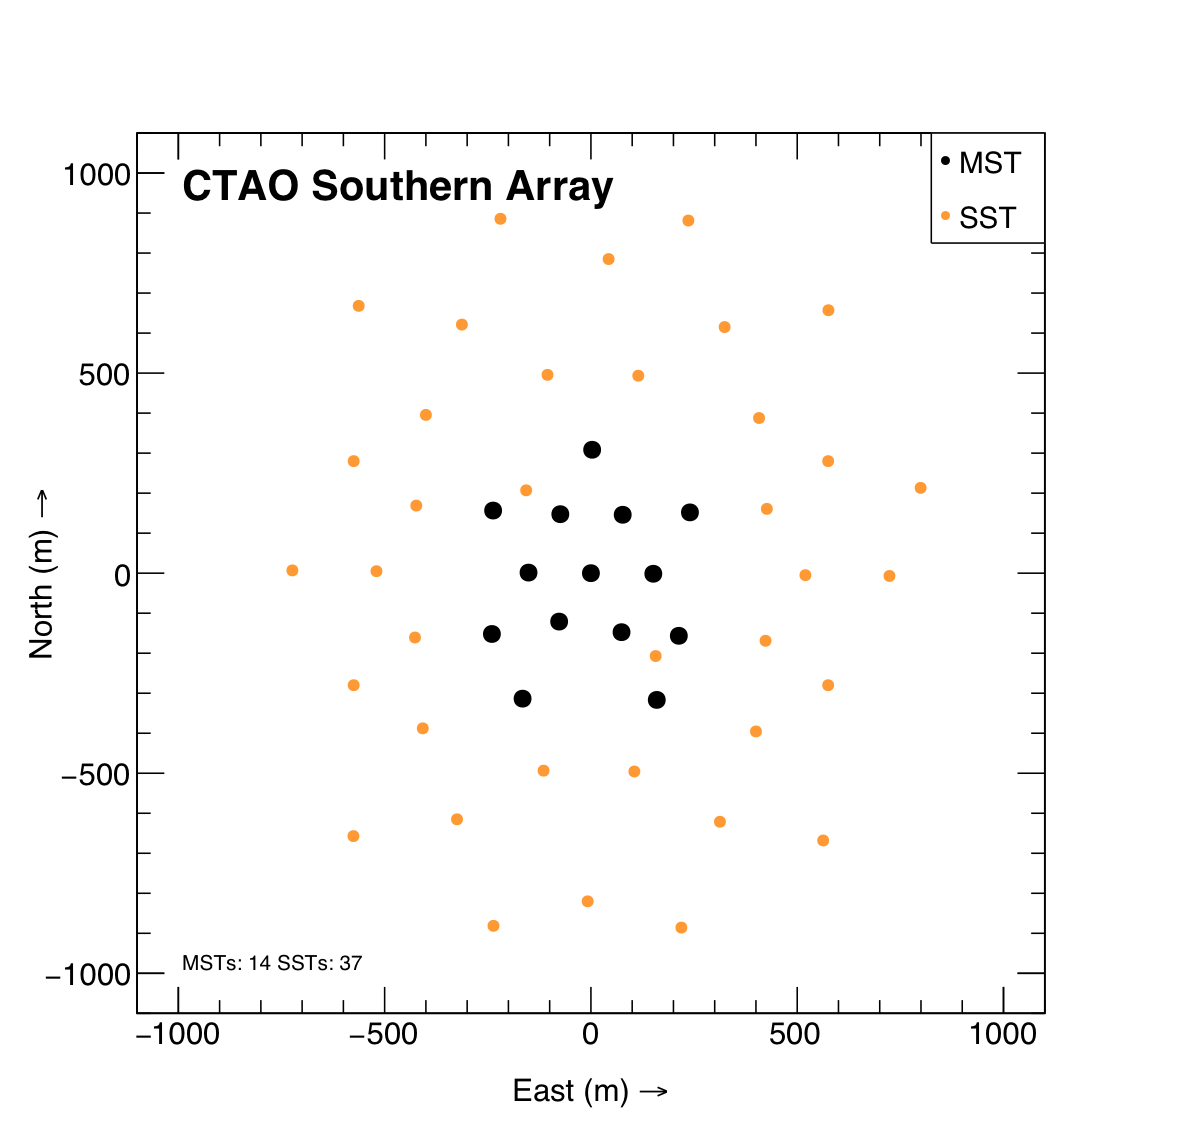
\includegraphics[width=0.7\columnwidth]{figures/southlayout.png}
        % note that in above figure file name, "sr_setup",
        % the file extension is missing. LaTeX is smart enough to find
        % apropriate one (i.e. pdf, png, etc.)
        % You can add this extention yourself as it seen below
        % both notations are correct but above has more flexibility
        %\includegraphics[width=1.0\columnwidth]{sr_setup.pdf}
        \caption{
                \label{fig:southlayout} % spaces are big no-no withing labels
                % things like fig: are optional in the label but it helps
                % to orient yourself when you have multiple figures,
                % equations and tables
                The CTA-South alpha array configuration, taken from \cite{zencta}.
        }
\end{figure}
\subsection{CHEC}
\begin{figure}[ht] 
        % read manual to see what [ht] means and for other possible options
        \centering 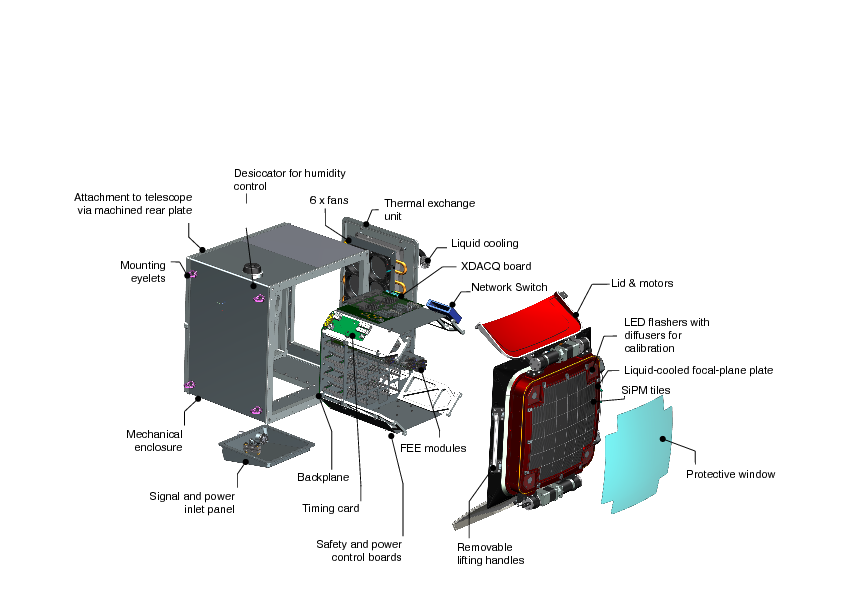
\includegraphics[width=\columnwidth]{figures/cam.png}
        % note that in above figure file name, "sr_setup",
        % the file extension is missing. LaTeX is smart enough to find
        % apropriate one (i.e. pdf, png, etc.)
        % You can add this extention yourself as it seen below
        % both notations are correct but above has more flexibility
        %\includegraphics[width=1.0\columnwidth]{sr_setup.pdf}
        \caption{
                \label{fig:cam} % spaces are big no-no withing labels
                % things like fig: are optional in the label but it helps
                % to orient yourself when you have multiple figures,
                % equations and tables
                The CHEC-S Computer Aided Design (CAD) model with key elements highlighted, taken from \cite{rwhite}.
        }
\end{figure}
The UK's main material contribution to CTA construction is planned to be construction of 13 SST Cameras (SSTCAMs). These are an upgraded version of the earlier Compact High Energy Camera (CHEC) prototypes, which were designed to work with SST structures that have a dual-mirror (Swartzchild-Couder) optical design. This design allows for a compact camera (approximately 0.4 m diameter) with small scale photosensors (6/7 mm, corresponding to roughly a third of the plate scale of a comparable single mirror design) and a wide field of view ($\sim$0.2 degrees per pixel).  Two operational CHEC prototypes have already been built. The first, CHEC-M, has as its light detectors 32 Multi-Anode Photomultipliers (MAPMs)\cite{tomthesis}. These consist of a block of 8x8 pixels, the signals from which are digitised at a rate of $1\mathrm{GSa}/\mathrm{s}$ \cite{tomthesis} by front end electronics based upon the custom TARGET application-specific integrated circuit (ASIC) \cite{checmpaper}. These blocks of front end electronics per SiPM tile are known as  a TARGET module (TM). When it is triggered by two or more four pixel blocks (superpixels) exceeding a discriminator threshold, the data is read out of the `fast chain' of the camera over a configurable window in blocks of 32 samples (roughly corresponding to a ns each). CHEC simultaneously has a slow-signal chain with a longer integration window in order to detect stars for pointing calibration. A refined prototype, CHEC-S, is currently undergoing testing at the Max Planck Institute for Nuclear Physics in Heidelberg. CHEC-S contains a refinement of the TARGET-based electronics of its predecessor, but replaces the MAPMs with SiPMs. These have the advantage of being more durable than MAPMs, as well as having a less notable drop in Photon Detection Efficiency (PDE) over time \cite{factphotonstream}; they are also cheaper and (crucially) can operate in conditions with a higher Night Sky Background (NSB) compared to MaPMs. CHEC-S also has a curved front window that helps to attenuate NSB whilst transmitting Cherenkov light \cite{ssticrc}. A final prototype SSTCAM engineering camera is currently undergoing construction, and will be the first SST camera delivered to CTAO.

Both CHEC cameras and the upcoming SSTCAM have inbuilt self-calibration LED flasher systems, designed to flat-field the camera. The flashers on the CHEC prototypes were attached to the camera corners and reflected off the secondary mirror, for the final SSTCAM design the flasher will most likely be situated behind the secondary mirror and shine through. CHEC additionally has a slow-signal analysis chain to perform simultaneous longer exposures on the sky, this allows for bright stars to be imaged and therefore used for online pointing calibration.

\subsection{GCT, ASTRI and the SST Harmonization Process}

There are two SST dual-mirror prototype SST designs that CHEC cameras can be attached to, the French led \textit{Gamma Cherenkov Telescope} (GCT), and the Italian led \textit{Astrofisica con Specchi a Tecnologia Replicante Italiana} (ASTRI) instrument. Both share a Schwartzchild-Couder optical design, which allows for a compact SiPM camera as well as a more uniform Point Spread Function (PSF) across the Field of View (FoV). Following a harmonisation process, the ASTRI optical design with a CHEC-type camera was selected as the basis for the final SST design, taking into account lessons learned from all prototypes. But for the purposes of the results in this thesis (which are primarily concerned with the camera), these two optical structures are largely interchangeable (in Chapter \ref{ch:3-TimingInfo} we consider CHEC-S with GCT as our instrument, whereas in the later  Chapter \ref{ch:5-CHECNSB} we consider CHEC-S on ASTRI). For the purposes of most of the work in this thesis, we consider CHEC-S to be broadly representative of the final SSTCAM, as the pixel sizes and configurations (the biggest influence upon our analysis) will likely be very similar.

\begin{figure}[ht] 
        % read manual to see what [ht] means and for other possible options
        \centering 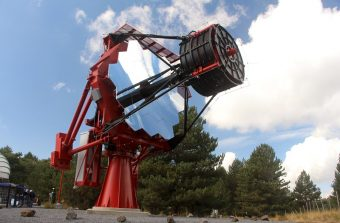
\includegraphics[width=\columnwidth]{figures/astri-horn.jpg}
        % note that in above figure file name, "sr_setup",
        % the file extension is missing. LaTeX is smart enough to find
        % apropriate one (i.e. pdf, png, etc.)
        % You can add this extention yourself as it seen below
        % both notations are correct but above has more flexibility
        %\includegraphics[width=1.0\columnwidth]{sr_setup.pdf}
        \caption{
                \label{fig:astri} % spaces are big no-no withing labels
                % things like fig: are optional in the label but it helps
                % to orient yourself when you have multiple figures,
                % equations and tables
                The ASTRI-Horn prototype on Sicily. Image Credit: CTA Collaboration.
        }
\end{figure}

\section{Types of IACT Backgrounds}
\subsection{Hadronic Air Showers}

In order to perform all of the scientific investigations explored in the previous section, along with the guest observation program, we need to be able to distinguish astrophysical gamma-ray signals from background reliably. Not all EAS in the atmosphere are caused by incident $\gamma$-ray photons. For most energies, EAS caused by incident charged hadrons (most commonly protons) outnumber those caused by photons by a factor of roughly 10,000 \cite{Benbow}. These provide a significant background to IACTs, and are the largest constraint on their sensitivity, as at IACT energies charged cosmic rays (protons, electrons and heavier nuclei) cannot be traced back to their origin due to scattering in the galactic magnetic field.

\begin{figure}
\begin{center}  

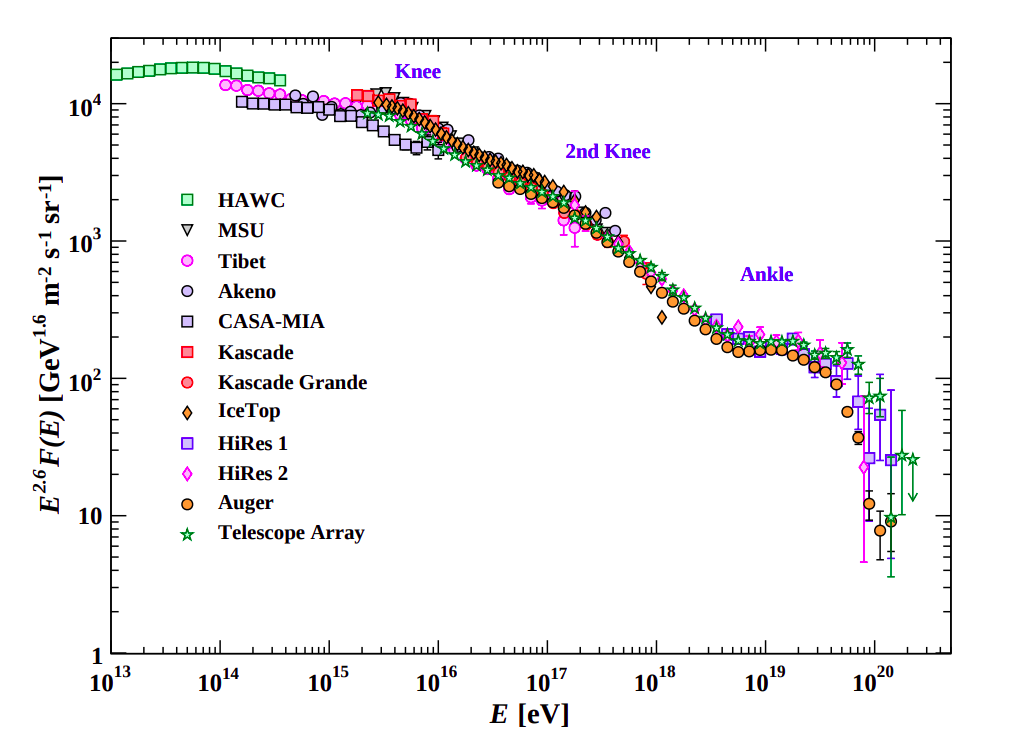
\includegraphics[width=\columnwidth]{figures/pdgcr.png}
 
\caption{The all particle cosmic ray spectrum, taken from \cite{pdg}. Whilst mainly protons, this spectrum includes both cosmic ray electrons and heavier element cosmic rays. The spectrum is a power law with index -2.7 up to around $3 \times 10^6$ GeV, where it steepens to an index of -3.1, a transition feature known as 'the knee'. It then flattens back to an index of -2.7 at $4 \times 10^9$ GeV (a feature known as 'the ankle'. The lower energy cosmic rays below the knee are believed to be galactic in origin, most likely a result of acceleration in supernova remnants. The higher energy cosmic rays above the knee are believed to be the result of cosmic ray acceleration in extragalactic sources such as Active Galactic Nuclei (AGN). The so-called GZK cutoff is theorised to exist at energies around 50 EeV \cite{gzk}, the limit at which a cosmic ray could propagate from another galaxy without interacting with the CMB. For comparison, the LHC operates at a centre of mass energy of 14TeV for proton-proton collisions, corresponding to an initial EAS proton energy of $1\times 10^{17}$eV.}
\label{fig:crspec}
\end{center}
\end{figure}

However, because the quarks contained within protons experience the strong nuclear force, the typical interactions they undergo on entering the atmosphere are different to photons. The collision of two sufficiently high energy protons can create pions through strong interactions.  A typical interaction scheme \cite{EAS} is
\begin{gather*}
\mathrm{p}+\mathrm{p}\rightarrow \mathrm{N}+\mathrm{N}+n_1 (\mathrm{\pi^+ + \pi^- }+n_2\mathrm{\pi^0} \\
\mathrm{\pi^0} \rightarrow \mathrm{2\gamma} \\
\mathrm{\mathrm{\pi^{\pm}}} \rightarrow \mathrm{\mu^{\pm}}+\mathrm{\overset{(-)}{\nu_{\mu}}}\\
\mathrm{\mu^{\pm}} \rightarrow \mathrm{e^{\pm}}+\mathrm{\overset{(-)}{\nu_{\mu}}}+\mathrm{\overset{(-)}{\nu_{e}}}
\end{gather*}
where $N$ represents the resulting fragmented hadrons which are produced along with $n_1$ charged pions and $n_2$ neutral pions. The charged pions have a lifetime of which have a short lifetime of only 26 ns, but the neutral pions' lifetime is much shorter at $5 \times 10^{-17} \mathrm{s}$ because it decays due to the electromagnetic force. Kaon production is also possible at higher energies, though the resultant products are the same. The rest frame lifetime of the muons is only 2.197 $\mu$s \cite{pdg}, however because the muons produced in these interactions are highly relativistic, the muons can survive to ground level as a results of time dilation effects. Some also decay to electrons via the weak nuclear force. The muons also undergo a significant number of inelastic scattering interactions, carrying a larger fraction of the total transverse momentum away from the shower core and resulting in a wider overall EAS compared to a $\gamma$-ray induced shower \cite{tomthesis}.  The resultant $\gamma$-rays from $\pi_0$ decay can themselves undergo pair production creating electromagnetic sub-showers of the hadronic shower core. The charged products are typically highly relativistic and thus produce detectable Cherenkov light.  Whilst the interaction scheme for hadronic air showers is more complex than for $\gamma$-ray or electron induced ones, it is still possible to construct semi-analytic models of their evolution. The most notable of these is the Heitler-Matthew model, details regarding this can be found in \cite{heitler}. As we'll see later in this chapter, hadronic interactions can similarly be undergone in astrophysical environments.
\begin{figure}[h!]
\begin{center}  

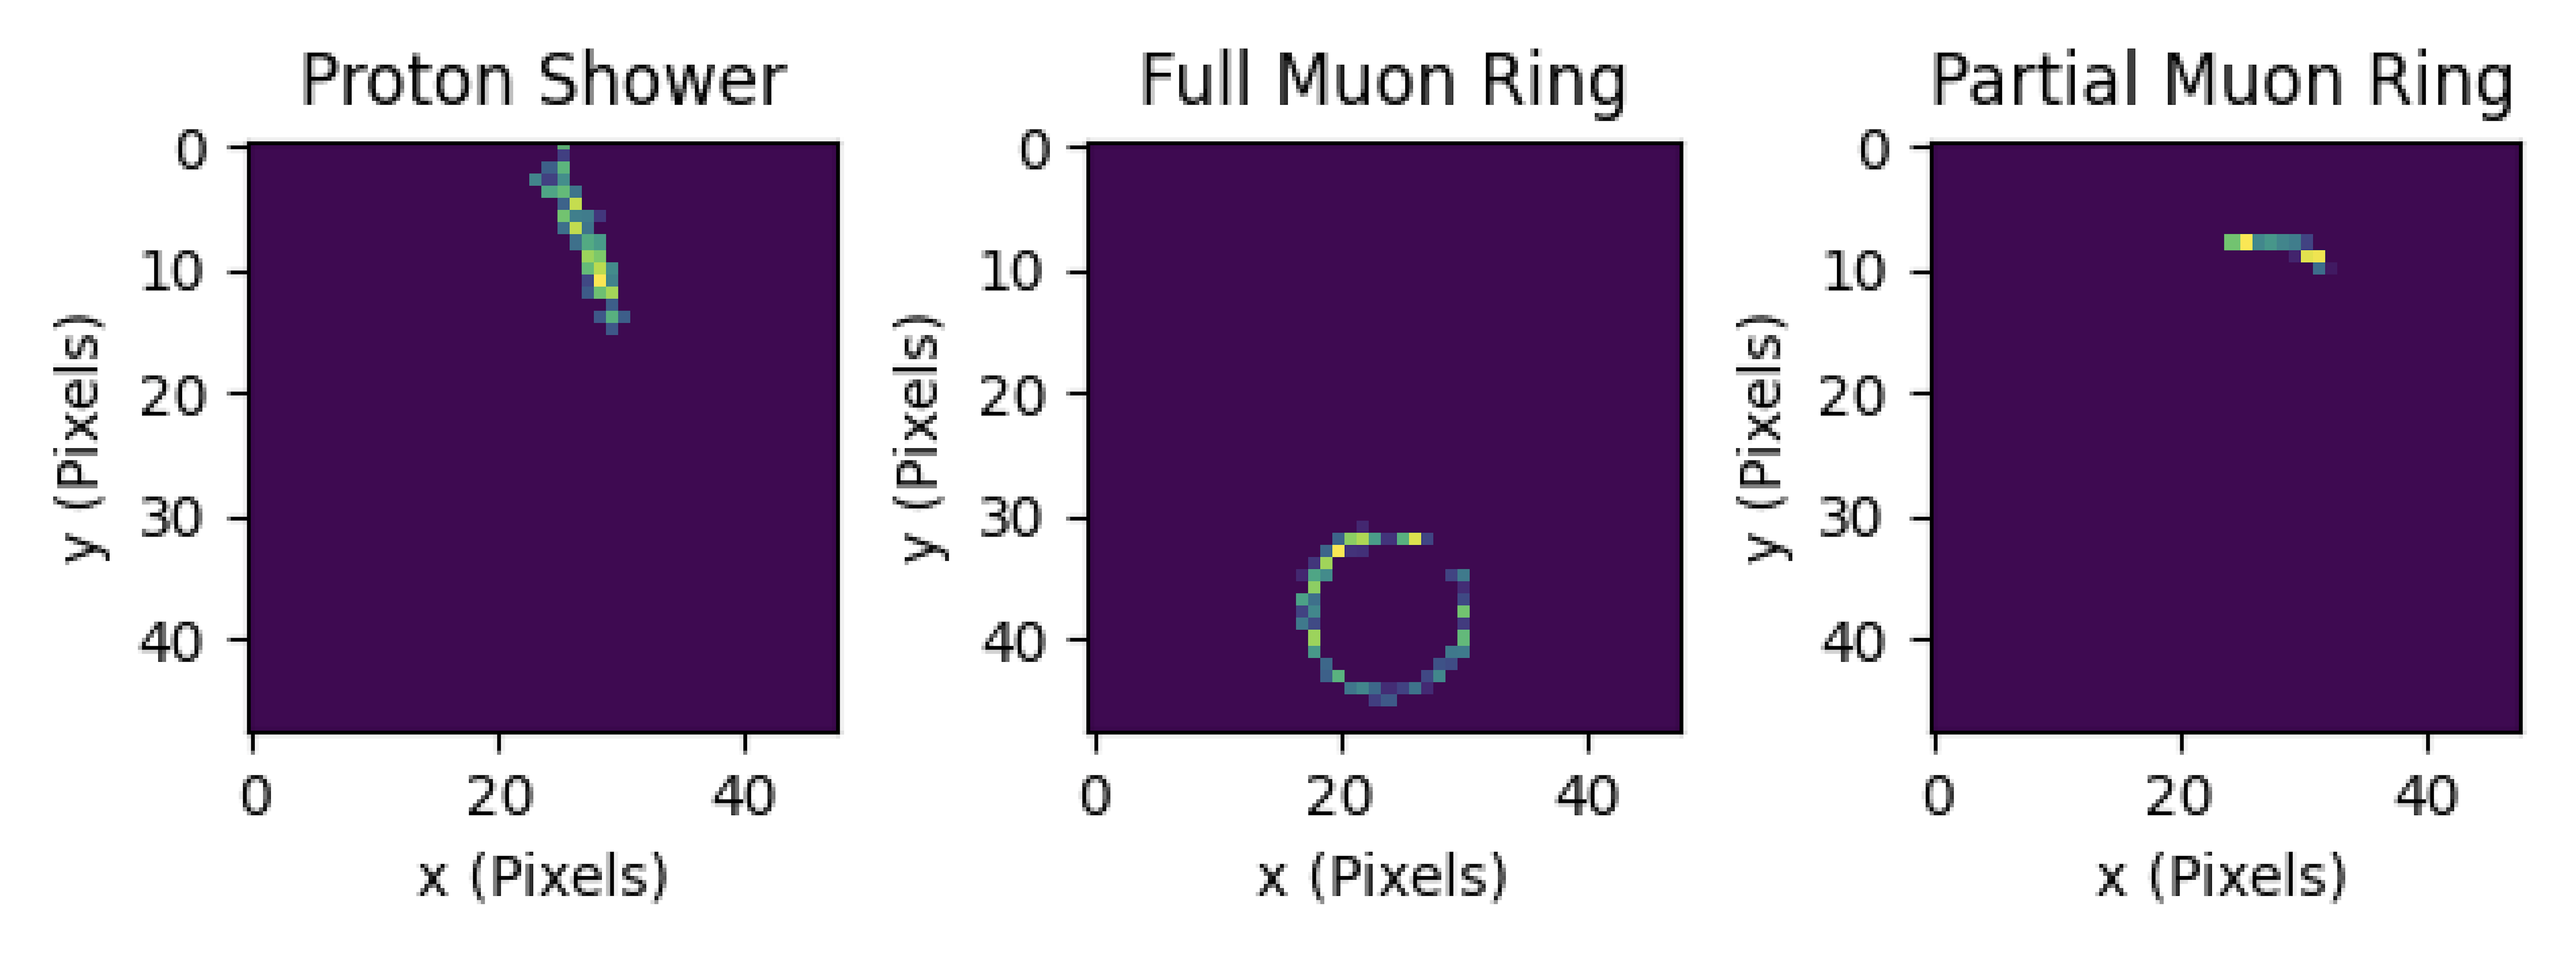
\includegraphics[width=\columnwidth]{figures/muonplot.png}
 
\caption{A proton shower image, a full muon ring image, and a partial muon ring image. These were generated using \textit{CORSIKA}/\textit{sim\_telarray} simulations of CHEC-S on ASTRI. The partial muon ring effect was generated by changing the impact distance from the telescope using the \textit{CORSIKA} CSCAT parameter.}
\label{fig:muonplot}
\end{center}
\end{figure}

Muons that survive to ground level and that pass directly along the optical axis of the telescope create characteristic `ring' images in the camera. These muon rings are useful for online calibration as the width of the muon ring image is proportional to the incident particle energy. The observed pixel intensity can then be compared to the expected intensity for a muon with that energy and can thus be used to compute the optical efficiency of the telescope system. Muons that pass off-axis to the telescope are only partially imaged; at sufficiently large impact parameters these partial muon ring images can closely resemble those of $\gamma$-ray EAS, creating an additional source of background. An example of such images can be seen in Figure \ref{fig:muonplot}.

\begin{figure}
\begin{center}  

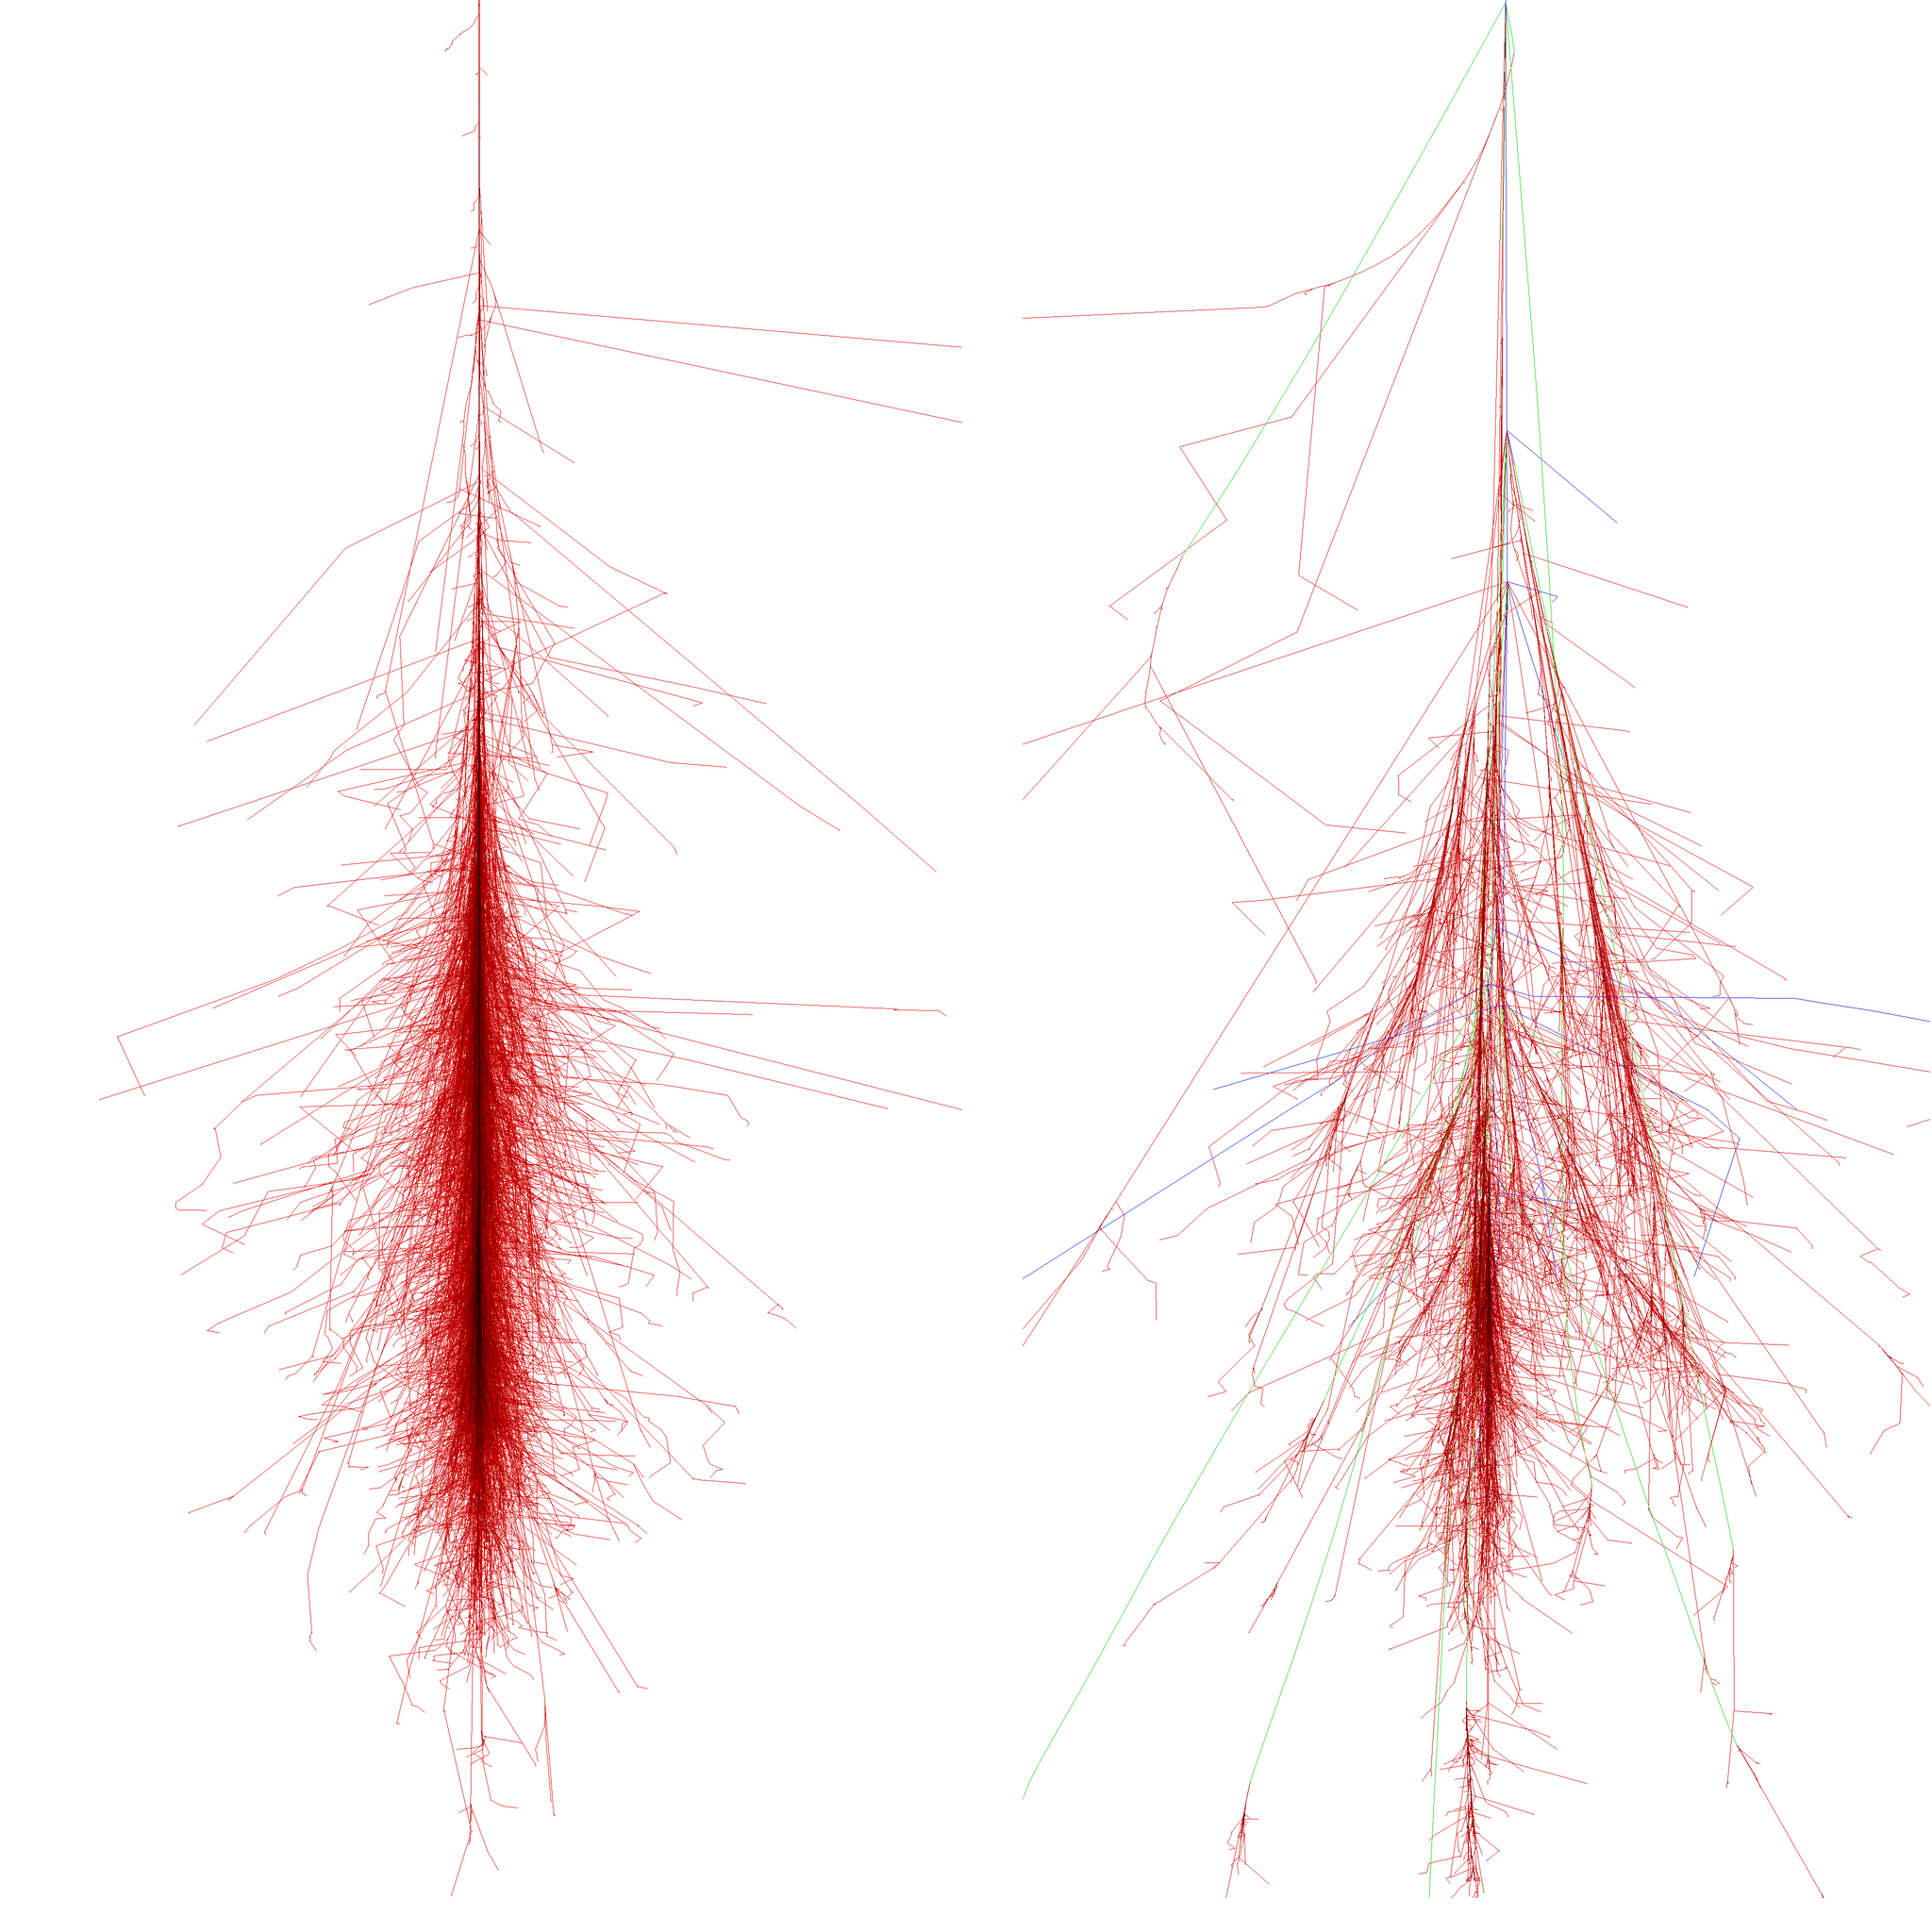
\includegraphics[width=\columnwidth]{figures/showers.png}
 
\caption{XZ plots of \textit{CORSIKA} simulations of particle tracks for 100 GeV photon (left) and proton (right) events. $\mathrm{e^+,e^-}$ and $\gamma$-rays are shown in red, $\mathrm{\mu^+\ and\ \mu^-}$ in green, and hadrons in blue. Note the wider, less concentrated proton shower which contains muons and hadrons that the $\gamma$-ray shower lacks (taken from \cite{corskplot}).}
\label{fig:image2}
\end{center}
\end{figure}
\subsection{Electron Air Showers}

In addition to the charged hadrons previously discussed, electrons can also be a significant source of background at low TeV energies. This is as they are difficult to distinguish from $\gamma$-rays and undergo similar interactions. There are two small differences between electron and $\gamma$-induced air showers. The first is the process by which the primary particles interact on hitting the atmosphere, a primary $\gamma$-ray will typically loose all its energy in a single pair production event. A primary electron of the same initial energy can loose energy via production of numerous lower-energy Bremsstrahlung photons which can create electromagnetic sub-showers. This can create a relatively greater number of Cherenkov photons at higher altitudes for electron-induced showers. The other small difference between electron and $\gamma$-ray induced showers is the average altitudes at which they first interact \cite{Sitarek1i}, which is due to the radiative length of an electron being smaller than the pair production length of a $\gamma$-ray. As a result, a primary cosmic-ray electron of the same energy as a primary $\gamma$-ray will begin interacting higher in the atmosphere. This results in a higher-altitude shower maximum \cite{lypova}. 

\subsection{Night Sky Background}
Not all of the background to an IACT can be attributed to other EAS. Night Sky Background (NSB), which refers to the light detected in Cherenkov camera images that is not attributable to Cherenkov light, is complex and in general, poorly modelled and understood. It consists of photons from a variety of sources (including, but not limited to)

\begin{itemize}
    \item Atmospheric air glow emission lines, particularly from atomic oxygen, hydroxide and sodium
    \item Moonlight
    \item Starlight and light from satellites
    \item Zodiacal light, along with diffuse galactic light and extragalactic background light (though these contributions are small) \cite{nsbref}
    \item Light pollution from population centres
\end{itemize}

Historically, analytic studies of NSB have been limited, as the standard \textit{CORSIKA} and \textit{sim\_telarray} simulation packages do not attempt to model NSB in a realistic way (for entirely legitimate reasons of computational cost). Most previous work on NSB has focused on direct observations with photomultipliers \cite{BandE}. We investigate the potential of advanced NSB modelling and how it might aid deep learning analysis in Chapter \ref{ch:5-CHECNSB}.

\section{Standard IACT Stages of Event Analysis}\label{app:imaging}
Now that we have established the basics of IACT operation and analysis, we turn to describing the stages that transform IACT event images into high-level astrophysical data.
\subsection{Trigger Selection}

Trigger selection is the first step in an IACT analysis chain. It is a feature of an IACT array designed to automatically reject events with a low probability of being astrophysical gamma-rays in the readouts of the camera. CHEC-S, for example, only reads out the camera photomultipliers if two adjacent superpixels (blocks of four adjacent pixels) passes a comparator check. The VERITAS trigger is slightly more complex. It consists of a single pixel trigger which acts on individual pixels (and includes timing analysis), a camera level trigger which works on the pattern and relative timing of the single pixel triggers, and an array trigger which requires that more than two telescopes are triggered in order such that an event is stored to disk\cite{veritastrigger}. This array-level trigger in particular significantly reduces the number of false triggers associated with muons passing through the instrument and telescope optics, as it is unlikely a single cosmic ray muon will generate sufficient Cherenkov light to trigger a second VERITAS telescope a few tens of meters away. A combination of trigger selection and simple parameter-based cuts can reduce the signal to background ratio to $\sim$ 1:1 for a bright source like the Crab Nebula using a current generation instrument like H.E.S.S. \cite{Berge07}.

\subsection{Pedestal Subtraction/Calibration}

After trigger selection, the next step is low level calibration. Electronic noise present in IACT camera data needs to be removed. For this purpose, measurements of the camera noise are taken when the camera is shut off from the outside environment with the shutter closed (similar to dark framing for optical astronomy). These measured pedestals are then subtracted from the observed live data. Flat-fielding of Cherenkov cameras is also necessary; it is typically performed by firing blue LED flasher units with known intensity profiles at the cameras.

\subsection{Charge Integration}

Once the raw data has been calibrated, the total number of photons collected by the photomultiplier from the EAS must be measured. Charge integration is the process of taking a calibrated PMT trace and extracting the number of photoelectrons. Various schemes exist for performing this operation, CHEC/SSTCAM relies on a cross-correlation template fitting model developed by J. Watson \cite{jasonthesis}.

\subsection{Tailcut Cleaning}

The next step in a conventional IACT analysis is tailcut cleaning. Before conventional IACT event reconstruction and classification, the sensitivity of these tasks to features in images from NSB requires that the images from the Cherenkov cameras are cleaned. The standard method of doing this is tailcut cleaning with two thresholds, whereby a pixel is only included in the analysis if the number of photoelectrons in the pixel exceeds a given threshold, or if it is the neighbour of such a pixel and also has a greater number of photoelectrons than a (typically lower) second threshold \cite{hegratailcut}. These thresholds require optimisation to achieve a desired event rate, and the implementations of this procedure vary by instrument (see for example \cite{magictailcut} \cite{Benbow} \cite{magictime}). Alternatively methods based upon wavelet image cleaning have been proposed \cite{wavelet}, but these are far more rarely used in practice. One of the aims of deep-learning-based image analyses that we explore in Chapters \ref{ch:3-TimingInfo} and \ref{ch:4-VERITASRealData} is to avoid this tailcut cleaning step, as some light from the Cherenkov shower itself is sometimes lost, however previous attempts at performing deep learning without requiring this step have failed when the event classifier or reconstruction method is exposed to real observations. 

\subsection{Hillas Parameter Based Techniques for Event Classification}
\begin{figure}[ht] 
        % read manual to see what [ht] means and for other possible options
        \centering 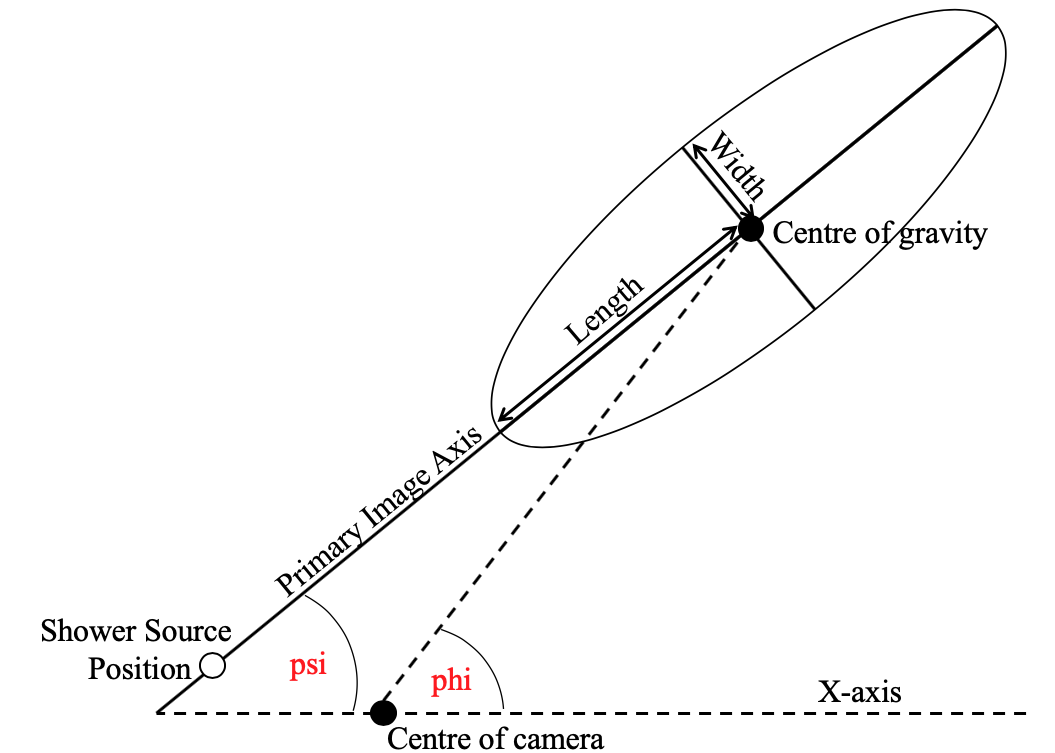
\includegraphics[width=\columnwidth]{figures/hillas.png}
        % note that in above figure file name, "sr_setup",
        % the file extension is missing. LaTeX is smart enough to find
        % apropriate one (i.e. pdf, png, etc.)
        % You can add this extention yourself as it seen below
        % both notations are correct but above has more flexibility
        %\includegraphics[width=1.0\columnwidth]{sr_setup.pdf}
        \caption{
                \label{fig:hillas} % spaces are big no-no withing labels
                % things like fig: are optional in the label but it helps
                % to orient yourself when you have multiple figures,
                % equations and tables
                The definition of Hillas parameters, taken from \cite{ctapipe}.
        }
\end{figure}
Hillas Parameters form the basis of the methods for event discrimination in the current generation of IACTs, and were instrumental in obtaining the first reliable gamma-ray source detection of the Crab nebula from the ground \cite{whipple} (much of the previous work in the years following 1953 centred on Pulsar detection and has since largely been disproved \cite{paulathesis}). They are obtained \cite{tomthesis} \cite{weekestev} from the second moments of an IACT camera image (constructed from the total integrated charge for each photomultiplier pixel), defined as 
\begin{align*}
\langle x^2 \rangle = \frac{\sum_i I_i x_i^2}{\sum_i I_i} && \langle y^2 \rangle = \frac{\sum_i I_i y_i^2}{\sum_i I_i}
\end{align*}
where $x_i$ and $y_i$ are the pixel co-ordinates and $I_i$ the associated pixel intensity. From these and the expectation values of $x$ and $y$ one can construct the variance and covariance
\begin{align*}
\sigma_x^2=\langle x^2 \rangle - \langle x \rangle^2&&\sigma_y^2=\langle y^2 \rangle - \langle y \rangle^2&&\sigma_{xy}=\langle xy \rangle - \langle x \rangle\langle y \rangle
\end{align*}
and define the following quantities
\begin{align*}
d=\sigma_x^2-\sigma_y^2&&a=(d+\sqrt{d^2+4\sigma_{xy}^2})/2\sigma_{xy}.
\end{align*}
The Hillas Parameters relevant for event classification are the width and length of the ellipse which characterize the transverse and lateral development of the shower and are defined by
\begin{align*}
W=\sqrt{\frac{\sigma_y^2+a^2\sigma_x^2+2a\sigma_{xy}}{1+a^2}}&&L=\sqrt{\frac{\sigma_x^2+a^2\sigma_y^2+2a\sigma_{xy}}{1+a^2}}.
\end{align*}
In order to take into account information from all of the telescopes in the array, these parameters must be combined into the Mean Reduced Scaled Width and Length (MRSW/MRSL), defined by a sum over all telescopes such that
\begin{align*}
SW&=\frac{W-\langle W \rangle}{\sigma_W}   &    SL&=\frac{L-\langle L \rangle}{\sigma_L}\\
\\ MRSW&=\frac{1}{\sum \omega}\sum SW\cdot \omega & MRSL&=\frac{1}{\sum \omega}\sum SL\cdot \omega
\end{align*}
where $\sigma_W$ is the spread of the expected width which must be obtained from Monte-Carlo generated lookup tables and $\omega=\langle W \rangle^2/\sigma_W^2$ is a weighting factor to take into account these tables' accuracy.

Initially Hillas Parameters were simply used to perform data cuts to separate hadronic showers from $\gamma$-ray induced showers based on their differing morphology. In recent years, more sophisticated methods using Boosted Decision Trees (BDTs) or Random Forests (RFs), which are essentially an extension of such cut based methods (taking the MRSL, MRSW, total integrated charge and other parameters derived from Monte-Carlo lookup tables), eventually became the preferred methods for incident particle classification \cite{hessbdt}. For $\gamma$-hadron separation, H.E.S.S. \cite{hessbdt} and VERITAS \cite{evdisp} typically use BDTs whereas MAGIC normally uses RFs. An example of the binary tree structure used for IACT event classification can be seen in Figure \ref{fig:bdtstruct}, whereby an event is classified as signal or background based on whether its input parameters pass a series of cuts (which can be optimised). Both BDT and RF methods both use an ensemble of trees to achieve superior performance. BDTs iteratively improve tree performance by increasing the weighting for events that we misclassified by the previous tree in all subsequent trees. In the common Adaboost BDT optimisation algorithm, this weighting factor $\alpha$ is given by 
\begin{equation}
    \alpha=\frac{1-\mathrm{err}}{\mathrm{err}}
\end{equation}
where $\mathrm{err}$ is the fraction of misclassified events in all leaves (endpoints in Figure \ref{fig:bdtstruct} of the decision tree \cite{hessbdt}. In RFs, a similar effect as achieved by randomly selecting a subset of input features at each node’s splitting point. One of the greatest advantages of decision-tree-based methods is that it is comparatively trivial to determine features in the input data that contributed to a classification; typically for IACT data the most important feature is the MSCW, but at energies below 100GeV estimation of shower maximum can be important \cite{hessbdt}. These feature importances are not as trivial to obtain for the deep learning methods we will encounter in later chapters. BDTs and RFs can also be used to perform directional and energy reconstruction for an event; for further technical details regarding the application of BDTs and RFs to IACT data see \cite{Sitarek1i} \cite{magictime} \cite{hessbdt} \cite{supermagictime} .

Hillas parameter based techniques don't however take advantage of the full camera image of the EAS, and as such, subtle details (such as hadronic `halos' \cite{model++}) in the images are not taken into account. This becomes an issue at the sensitivity boundaries that CTA is aiming to considerably improve (particularly in the case of weak or very extended sources), as hadronic and electron induced showers at these energies can closely resemble those generated by $\gamma$-rays. This motivates us to investigate new analysis techniques for event discrimination in order to improve the IACT sensitivity, as even small improvements to $\gamma$/hadron separation can translate into a significant increase in performance.

\begin{figure}[ht] 
        % read manual to see what [ht] means and for other possible options
        \centering 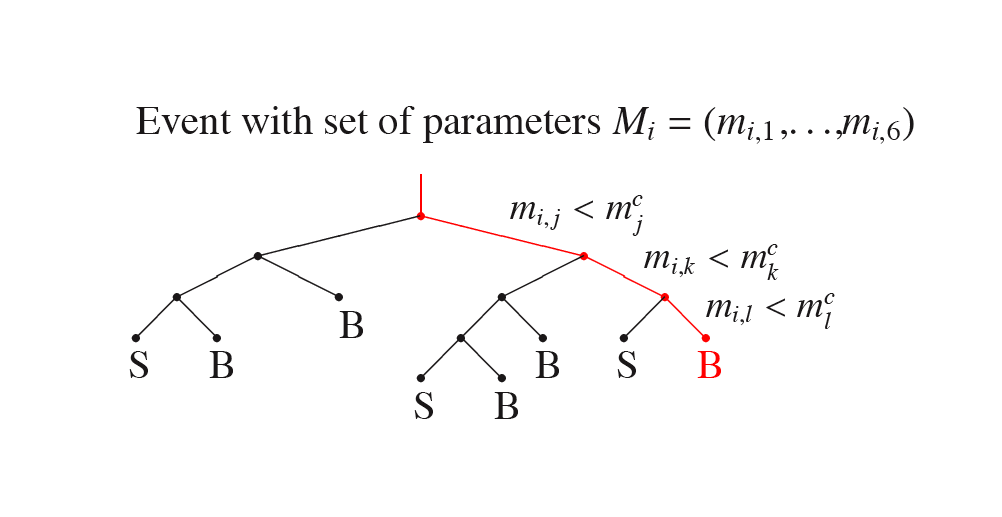
\includegraphics[width=\columnwidth]{figures/forest_picture.png}
        % note that in above figure file name, "sr_setup",
        % the file extension is missing. LaTeX is smart enough to find
        % apropriate one (i.e. pdf, png, etc.)
        % You can add this extention yourself as it seen below
        % both notations are correct but above has more flexibility
        %\includegraphics[width=1.0\columnwidth]{sr_setup.pdf}
        \caption{
                \label{fig:bdtstruct} % spaces are big no-no withing labels
                % things like fig: are optional in the label but it helps
                % to orient yourself when you have multiple figures,
                % equations and tables
                An example of a BDT, taken from \cite{hessbdt}. The event is classified as either Signal (S) or Background (B) by the tree based on whether at each node on the tree the parameters $m_{i,j}$ are larger than the weights $M^c=(m^c_j,...)$. The ultimate event classification is not performed by one tree, but by the weighted mean of an ensemble of trees generated iteratively by evaluating the trees' efficiency against training data.
        }
\end{figure}

\subsection{Event Selection Cuts and Run Selection}

IACT observations are normally conducted in runs, where the IACT array tracks and observes a single source. The length of these runs varies, but most IACT observatories use between 20 and 30 minutes. This is as to obtain a sufficient number of events to accurately model background, whilst observation conditions are roughly constant.

Most IACT analysis begins with Hillas parameter cuts on the data to remove obviously hadronic events (with very high MRSW) and events far from the desired source (so-called theta squared cuts). It is also common to remove runs or events from an IACT analysis for a variety of reasons. The data from a run may be low quality due to poor weather conditions, hardware or tracking issues or high zenith angle (where simulation accuracy drops due to the complexity of modelling the atmosphere correctly). Most IACT analyses use multiple runs per source, though the work in Chapter \ref{ch:4-VERITASRealData} considers only a single VERITAS run as we attempt to match the data more closely with simulations.

\subsection{ON/OFF Region and Reflected Region Analysis}
So far we have focused on Cherenkov camera based background rejection, however this only reduces the signal to background rate (by around a factor of 100) to $\sim$ 1:1 for bright sources. As such, there is a need for a higher level background rejection method, similar to aperture photometry in optical astronomy. The simplest method possible is to take one ON region and one OFF region at the same right ascension but differing declination and use this to compute the $\gamma$-ray excess. The disadvantage of this is the loss of time on source. An alternative developed by the Whipple observatory is so called `Wobble Mode', where the telescope wobbles around the source in declination, allowing for more time on source. However, this is complicated by two factors, the comparatively poor angular resolution of IACTs, and the significant extension of some sources such as the supernova remnant RXJ 1713.7-3946. As such, the HEGRA collaboration \cite{HEGRA} developed so called reflected-region analysis, where multiple non-overlapping OFF regions (at different distances from the ON region but of the same angular size) are used. This allows for better statistics compared to a singular OFF region and allows for measurement of a potentially non-uniform night sky background across the field. This is the technique we use in Chapter \ref{ch:4-VERITASRealData}. However, such methods can run into difficulties for very extended objects such as Geminga, as the size of the source emission region might exceed the size of the FoV \cite{geminga}. In such scenarios a `FoV' background model, which models the radial acceptance of the IACT system can be used. The technical details of this are beyond the scope of this thesis; for more detail we refer the reader to \cite{Berge07} and \cite{geminga}. 

\subsection{Pointing Corrections}
Also necessary for reliable IACT operation is pointing calibration, as the size of the telescopes means they can bend slightly \cite{veritasstat}. This is typically performed by reconstructing the positions of stars using CCDs attached to the telescope structure, though SSTCAM has a slow signal chain to perform this (we explore the consequences of this in Chapter \ref{ch:5-CHECNSB}). This allows for positions of $\gamma$-ray sources to be reconstructed to within 2-3'; this can be of important, especially for sources with extended morphology \cite{cena} \cite{rxjcta}.

\subsection{CTA Data Analysis Levels}

The proposed CTA analysis pipeline consists of a number of data analysis levels. Data processors exist to transform data at each level into the next. Only some of these levels are relevant for deep learning analyses. The current CTA data structure consists of \cite{jasonthesis}:
\begin{itemize}
    \item r0 data, which is the uncalibrated raw data generated by the Cherenkov camera.
    \item r1 data, which is online, calibrated camera data, calibrated using a scheme specific to the camera.
    \item dl0 data, which is calibrated waveform data along with event metadata, and is zero suppressed to save bandwidth and storage space.
    \item dl1 data, which consists of extracted charge and peak time information extracted from the calibrated waveforms, as well as Hillas parameters extracted from them.
    \item dl2 data, at this stage the telescope multiplicity is dropped and the overall events are characterised (based on their Hillas parameters extracted during the dl1 stage) into shower parameters including energy, direction, and source particle
    \item dl3 data, at this stage the dl2 events are sorted into sets of (for example) $\gamma$-ray candidates. This also includes any relevant instrument response data needed for higher level analysis.
    \item dl4 data, which consists of fully processed event lists, ready for high level astronomical analysis.
    \item dl5 data, which consists of high level analysis data products produced from astronomical analysis, such as the CTA galactic plane survey.
\end{itemize}

The CTA analysis chain will therefore reduce the raw amount of data from the telescopes from Petabytes to data scales tractable with a laptop.

\section{Alternatives to Hillas-Parameter-Based Techniques}
In this section we briefly consider the existing alternatives to Hillas analysis for IACT event classification and reconstruction.
\subsection{Template Analyses and Model++}
Template analyses \cite{model++} \cite{cat} \cite{3danalysis}  \cite{impact} form the current main alternative to Hillas parameterisation. They rely on the generation of a library of template IACT images. The images from the IACTs are then compared to the templates via a pixel-by-pixel minimisation process, such that the template most resembling the IACT image can be found and thus the shower properties inferred. In particular, the H.E.S.S. Model++ analysis chain uses chi-squared fitting against semi-analytic models of $\gamma$-ray showers as a background rejection method \cite{model++}. Whilst Model++ may be widely used within H.E.S.S., the reality that the authors of Model++ have chosen not to make their code open source means that it is not currently being considered as an analysis method for CTA, and its efficacy in the SST energy range has also not been tested. At the time of writing there is not a major effort within CTA to recreate it.

\subsection{ImPACT}
The most widely used template analysis is using the \textit{Image Pixelwise fit for Atmospheric Cherenkov Telescopes} (ImPACT) code \cite{impact}. This works by comparing the shower images to interpolated templates generated using Monte-Carlo simulations. ImPACT was developed for the (previously unprecedentedly large) H.E.S.S. CT5 telescope as Hillas parameter based techniques are known to be unreliable at photon energies lower than $50 \rm{Ge}V$.  The reconstructed event parameters are the combination of shower parameters for the template which minimizes the total negative log likelihood $\ln\mathcal{L}=\sum_{pixel,i}-2\ln{P(s_i|\mu,\sigma_p,\sigma_y)}$(maximizes the likelihood) over every pixel in the camera for every telescope in the array, where
\begin{equation}
P(s_i|\mu,\sigma_p,\sigma_y)=\sum_n \frac{\mu^n e^{-\mu}}{n!\sqrt{2\pi (\sigma_p^2+n\sigma_{\gamma}^2)}} \exp \left(-\frac{(s-n)^2}{2(\sigma_p^2 + n \sigma_{\gamma}^2)} \right)
\end{equation}
$n$ is the photoelectron number, $\sigma_p$ is the pedestal width (the width of the charge distribution under pure noise), $\sigma_{\gamma}$ represents the photomultiplier resolution, $s$ is the number of signal photoelectrons detected and $\mu$ is the predicted number of photoelectrons from the template. In practice, ImPACT is only used for directional and energy reconstruction in H.E.S.S. due to concerns about its sensitivity to NSB photons (a problem similar to the real observations problem experienced by Convolutional Neural Network (CNN)-type methods that we will explore in Chapter \ref{ch:4-VERITASRealData}). The H.E.S.S. ImPACT chain uses a BDT based on Hillas Parameters for $\gamma$/hadron separation. The ability of ImPACT to utilise stereoscopic sets of complete IACT images can significantly improve directional reconstruction compared to Hillas-parameter-based methods, especially at low energies \cite{impact}.

The difficulty in using ImPACT for CTA is the requirement of having a sufficient number of template simulations to cope with every possible type of event with a given energy and incident direction for a large number of telescopes, and the computational cost of searching through those simulations to find the optimal event parameters. That said, there is an open-source implementation of ImPACT available within \textit{ctapipe}.

\section{The Prototype CTA Analysis Chain and ctapipe}

CTA is an instrument that is currently in the development phase, and this is true both of the instruments and the analysis pipelines that go with them. For much of the writing of this thesis a full, pythonic analysis pipeline for CTA did not exist, and CTA analyses were a complex mixture of modern code and software written for previous instruments. Additionally, a detailed, complex Monte-Carlo validation procedure was underway relating to the simulated data for even the prototype cameras.

\textit{ctapipe} is a python-based tool developed as an open-source prototype (which follows modern code practices for version control and code development) for the low-level analysis of CTA data. It is now recognised as a critical tool for CTA pipeline development. It provides tools to both handle \textit{CORSIKA}/\textit{sim\_telarray} simulations, perform data calibration and charge extraction, and to extract Hillas and muon ring parameters for events. It also contains \textit{astropy} based tools to compute camera pixel positions on sky, needed for the NSB work we present in Chapter \ref{ch:5-CHECNSB}. \textit{ctapipe} can even be used to analyze data from existing and historical IACT arrays; elements of our VERITAS work in Chapter \ref{ch:4-VERITASRealData} used reverse engineered code from ctapipe.

\textit{gammapy} and \textit{ctools} are the current open-source prototypes for high-level analysis (following similar development practice to \textit{ctapipe}); of these \textit{gammapy} has been selected as the high-level science tool for CTA. These allow one to generate source significance maps, lightcurves and spectra using IACT event lists. For simplicity, our \textit{VERITAS} work utilised the older, more stable \textit{Eventdisplay} tools for the work presented in Chapter \ref{ch:4-VERITASRealData}. But in time, high level data from all existing IACTs could be analysed with these new open-source packages.

\section{Methods and Environments of Astrophysical \ensuremath{\gamma}-ray Emission}
\subsection{Inverse Compton Scattering}

In this section we briefly discuss the how and where astrophysical $\gamma$-rays are produced. The majority of astrophysical $\gamma$-rays are believed to be produced by Inverse Compton (IC) scattering. Inverse Compton scattering describes the process by which low energy photons are scattered by ultra-relativistic electrons, significantly increasing the kinetic energy of the photons. The photon fields accelerated by the electrons vary; they can be a population of photons produced through synchrotron emission that are then hit by the high energy electrons that emitted them (so-called synchrotron self-Compton emission), can be the result of starlight, or originate from the cosmic microwave background. In the rest frame of the electron, the ratio of final photon energy over initial energy is given by
\begin{equation}
    \frac{E_f}{E_i}=\gamma (1+\beta \cos(\theta))
\end{equation}
where $\gamma$is the Lorentz factor of the electrons and $\theta$ is the deflection angle. Transferring to the observer frame this works out at around $\frac{E_f}{E_i}\sim \gamma^2$. Using this, combined with considerations of the energy density of the photon field ($u_{rad}$ in the observer frame), it can be shown \cite{longair} that the energy loss rate from a relativistic electron travelling at speed $\mathrm{v}$ due to IC scattering is

\begin{equation}
    \left(\frac{dE}{dt}\right)_{IC}=\frac{4}{3}\sigma_T c u_{rad}\left(\frac{\mathrm{v}^2}{c^2}\right)
\end{equation}

This results in the spectral emissivity from IC scattering of an isotropic photon field of single photon frequency $\nu_0$ by a power law distribution of electrons being given by 
\begin{equation}
    I(\nu)d\nu=\frac{3\sigma_TcvN(\nu_0)}{16\gamma^4\nu_0^2}\left(2c\ln\left(\frac{\nu}{4\gamma^2\nu_0}\right)+\nu+4\gamma^2\nu_0-\frac{\nu^2}{2\gamma^2\nu_0}\right)dv
\end{equation}
where $N(\nu_0)$ is the number density of photons, $\sigma_T$ is the Thompson cross section and $\nu$ is the frequency of the $\gamma$-rays \cite{blumenthal}.


\subsection{Hadronic Emission}
The second method of producing astrophysical $\gamma$-rays is through hadronic interactions. As we saw for EAS, proton-proton interactions can produce $\pi^0$ particles which decay to a pair of $\gamma$-rays. Hadronic emission processes are challenging to discriminate from IC scattering in some sources, particularly supernova remnants \cite{rxjcta}. The recent detection of an astrophysical neutrino (IceCube-170922A) by IceCube that was coincident with a $\gamma$-ray flare of the blazar TXS 0506+056 suggests that some $\gamma$-rays from AGN are produced by hadronic processes, likely close to the associated supermassive black hole \cite{TXS}. 

\subsection{Supernova Remnants and Pulsar Wind Nebulae}
Now that we have considered the physical mechanisms by which astrophysical $\gamma$-rays are produced, let us consider the environments where this production might occur. Given the innately high energies involved, supernova remnants are prime sources of galactic $\gamma$-ray emission. Supernova remnants are also suspected of being one of the galactic sources of the highest energy cosmic rays (so-called PeVatrons). Most notably the supernova remnant RXJ1713.7-3946 has been detected to be spatially extended by H.E.S.S.; CTA might help to understand the emission mechanisms present in this source \cite{rxjcta}. Pulsar Wind Nebulae (PWN, also known as Plerions) such as the Crab Nebula are another, older related class of $\gamma$-ray sources where a wind from a central pulsar interacts with the surrounding ejecta to produce high-energy emission \cite{magiccrab}. A certain fraction of these PWN are so-called TeV Halos, highly-evolved (believed to be older than 100 kyr) systems where the pulsar has passed through the ejecta (after receiving a kick) from the associated supernova remnant and is now accelerating electrons in a spatially isolated region \cite{tevhalo}. Geminga is a likely candidate for such a system \cite{geminga}.

\subsection{$\gamma$-ray Binaries}
$\gamma$-ray Binaries are similar to their X-Ray counterparts, where a compact object (such as a neutron star or black hole) accretes matter from a companion star. $\gamma$-ray binaries differ from X-Ray Binaries typically because of the comparatively high mass of the companion star (typically an O or B class giant), as well as their higher-energy emission. Very few of these sources have been detected by IACTs ($\sim$7 at the time of writing), and they are generally fairly poorly understood \cite{scienceCTA}. CTA might help us to understand these objects.

\subsection{Active Galactic Nuclei}
AGN are known sources of GeV and TeV $\gamma$-rays, typically these are blazars (where the jet of the AGN directly points towards Earth). These blazars fall into two categories based on how energetic they are, these are known as BL LACs (for the low energy case) or Flat Spectrum Radio Quasars (FSRQs, for the high energy case). The characteristic double-peaked Spectral Energy Distribution (SED) of blazars is evidence for there being some synchrotron-self-Compton emission from these objects. Flares (unusual periods of bright emission) from AGN are also observed as a class of extragalactic $\gamma$-ray transient, see for example \cite{TXS}.

\subsection{Galactic and Extragalactic Transients}
GRBs are typically bright, but comparatively short lived in their $\gamma$-ray emission. These GRBs are believed to originate from neutron star collisions or core-collapse supernovae; differences in the redshift distributions of short-lived and long-lived GRBs is evidence to support this hypothesis \cite{longair}. GRBs have only recently been observed from the ground, partly due to the technical challenge of turning the instruments quickly enough to detect the prompt emission, but also due to the complex factors involved in background rejection and the fact that most GRBs do not have spectra extending into the TeV. The first detection of a both prompt emission from a GRB and lower-energy afterglow was comparitively recently, in 2019 \cite{magicGRB}.

The first galactic transient detected by an IACT was the recurring Novae RS Ophiuchi by H.E.S.S. [H.E.S.S. Collaboration, in prep], the emission was a result of a thermonuclear explosion of the surface of an accreting white dwarf. This detection was somewhat unexpeceted, but suggests CTA might be able to detect a greater population of galactic transient objects.

\subsection{Diffuse Emission}
Both galactic and extragalactic diffuse $\gamma$-ray emission are observered by IACTs. In the galactic case it is believed the majority of the emission results from hadronic emission due to collisions of cosmic rays with galactic gas \cite{extragamma}. The extragalactic case is less well understood \cite{extragamma}, with the majority of emission likely due to unresolved blazars, radio galaxies and star-forming galaxies, but some additional components may be due to dark matter annihilation or cosmic ray interactions.

\section{The Key Science Projects of CTA}
Now that we have determined the origin and production of $\gamma$-rays, we will briefly discuss the observing strategy for the scientific investigations of CTA. The CTA observing time not allocated to open observations or Target of Opportunity (ToO) observations will be dedicated to a number of Key Science Projects (KSPs). In this section we briefly explore the science potential for each of these missions.

\subsection{The Galactic Centre KSP}
CTA observations will be made of the central square degree of the Milky Way for 500 hours \cite{scienceCTA}, with a further 300 hours spent observing the region up to 10 degrees in galactic latitude. It is anticipated that this will be one of the first major campaigns for CTA due to its implications for other CTA surveys.
In particular, the galactic centre is considered one of the best places to search for evidence of dark matter annihilation, and these observations should be sufficient to obtain either a detection or an upper limit for many of the current best dark matter models \cite{scienceCTA}. Additionally, these observations hope to uncover the nature of the galactic centre $\gamma$-ray source, and to probe the nature of very high energy particle acceleration in the galactic centre (key to understanding the nature of the Fermi Bubbles). 

\subsection{The Galactic Plane Survey (GPS) and the Cosmic Ray PeVatron KSP}
Around 1800 total hours of observing time will be spent performing observations of the galactic plane, with a sensitivity of at least 4.2 mCrab \cite{scienceCTA} (an improvement of 5-20 times relative to current instruments). It is planned that this survey will lead to the discovery of new galactic sources of TeV $\gamma$-rays, including supernova remnants, $\gamma$-ray binaries and Pulsar Wind Nebulae. Additionally, it will provide new constraints for models of the galactic diffuse emission and source populations. 

It is anticipated that the maps generated by the GPS will be periodically made public, in order to maximize its multi-wavelength science potential.
Additionally, the PeVatron KSP aims to perform dedicated, deep observations of known $\gamma$-ray sources with particularly hard spectra (such as RX J1713.7-3946), and search for diffuse $\gamma$-ray emission around known Supernova Remnants in an attempt to understand the origins and acceleration methods of cosmic rays \cite{scienceCTA}.

\subsection{The Large Magellanic Cloud Survey and the Star Forming Systems KSP} Around 600 hours of CTA observation time will be spent on observing the Large Magellanic Cloud (LMC). In particular, the LMC is interesting at TeV energies due to its high rate of star formation; the LMC produces about one tenth of the number of stars as the Milky Way, but has only 2\% of the Milky Way's volume \cite{scienceCTA}.
As such, it contains a disproportionate number of supernova remnants (such as SN1987A) and pulsar wind nebulae.  These can be observed more easily in the LMC than in the Milky Way due to the absence of source confusion, interstellar absorption and line of sight crowding at the LMC's high galactic latitude \cite{scienceCTA}. Other observations of galactic star forming regions (for example Westerlund 1) are also planned as part of the star forming systems KSP, in order to investigate the link between star formation and particle acceleration.

\subsection{The Extra-Galactic Survey and the AGN KSP} One of the largest time allocations, the extra-galactic survey will cover 25\% of the sky down to 6 mCrab sensitivity \cite{scienceCTA}. It will aim to achieve an unbiased census of $\gamma$-ray AGN, observe fast-flaring sources and gamma-ray busts serendipitously, and measure the anisotropies in the electron cosmic ray spectrum. Key to this is CTA's ability to operate in a divergent pointing mode, where not all telescopes in the array are pointing at the same patch on the sky. 

An AGN KSP is also envisaged to perform long term monitoring of a select set of Active Galactic Nuclei, in order to understand how the different types of AGN are related, and how their particle and $\gamma$-ray acceleration mechanisms work \cite{scienceCTA}. By extension, these observations should also act as a probe of the intergalactic magnetic field and the extragalactic background light. The AGN KSP is also a means of performing tests of fundamental physics, and CTA should be able to place constraints on Lorentz Invariance Violation and the production of Axion-like particles through the monitoring of AGN. 

\subsection{The Transient KSP} Somewhat intertwined with the Extra-Galactic Survey, CTA will have the capability to respond to transient events from both internal and external triggers. These external triggers will be sent by Gravitational Wave, Neutrino, Radio, Optical, X-ray and $\gamma$-ray observatories around the world when they detect a transient object. Following such a trigger, CTA will immediately perform follow-up observations to help constrain the emitting object's nature \cite{scienceCTA}. Likewise notifications of transient events serendipitously detected by CTA will be sent to partner observatories.

\section{Thesis Structure}
The remainder of this thesis is structured into five chapters. In Chapter \ref{ch:2-CNNs}, we introduce deep learning methodologies, before exploring past and concurrent work on their applications for IACTs, and then introducing multiple problems with such applications that are currently unsolved. In Chapter \ref{ch:3-TimingInfo} we explore the previously unconsidered option of utilising photosensor timing information as a basis for a deep learning event classification method, utilising the advanced capability of waveform storage possible with SSTCAM. In Chapter \ref{ch:4-VERITASRealData}, we explore the difficulties in using charge-based deep learning classifiers with existing data from VERITAS, exploring in detail the complication of optimising deep learning classifiers and the complexities arising from not wishing to perform tailcut image cleaning. Chapter \ref{ch:5-CHECNSB} concerns a detailed study into the likely NSB conditions experienced by SSTCAM. Whilst NSB represents a significant challenge to deep learning event classification and reconstruction methods, the work within this chapter is largely self-contained. Finally in Chapter \ref{ch6-Conclusions} we investigate future prospects for analyses in these fields and conclude.
\chapter{\label{ch:2-CNNs}Deep learning methods and their applications for IACTs}
\minitoc
\begin{abstract}
    Deep learning analysis methods based upon CNNs are becoming increasingly widely utilised throughout the physical sciences. In this chapter we explore the basic properties of such methods, before reviewing past and concurrent work on utilising these methods with IACT data. We then go on to explore the known issues with these methods in depth.
\end{abstract}

\section{Introduction}

Machine learning has been critical to the operation of the current generation of IACTs, H.E.S.S., MAGIC and VERITAS. As explored in Chapter \ref{ch:1-intro}, BDT-based methods used currently have offered a significant sensitivity improvement over conventional Hillas parameter cuts alone. However, when dealing with a new generation of IACT cameras with improved pixel density and timing precision, these BDT methods have notable shortcoming. This is that they do not take account of all the image and timing information available to them. This is a very similar situation to IACT astronomy in the early 2000s, as the construction of the current generation of IACTs with larger cameras necessitated the development of BDT and template fitting techniques. As such, the machine learning task force in CTA was set up to investigate whether it is possible to obtain a sensitivity improvement for CTA by using new deep learning techniques. At the same time, deep learning is a very rapidly advancing field, new models and methods of handling data are constantly becoming available (see for example \cite{adithesis} \cite{chebnet}), but these new methods must be adapted and tempered for IACT analysis. In this chapter, we explore the current state of the art in machine learning methods in greater depth, before going on to explore past work on implementing newly available deep learning techniques for IACT data, and some of the problems that have already been found. 

New deep learning methods, which are neural network methods with many layers, or equivalently a high degree of feature abstraction, are frequently associated with `AI'. Despite this, true emergent AI that can interpret universal input data and formulate meaningful responses remains science fiction, with no serious research currently being performed \cite{emergent}. In practice, most supervised deep learning techniques are simply an advanced form of pattern recognition, with weights being adjusted to provide known responses to known training data. When exposed to new data outside of their original training data sample these methods often run into difficulties, an area of computer science research referred to as `Domain Adaptation' \cite{wilson}. We will begin to encounter such difficulties in Chapter \ref{ch:4-VERITASRealData}.

\subsection{Types of Machine Learning}
Before addressing substantially the novel elements of this thesis, it is necessary for us to introduce a number of basic concepts and terms. \textbf{Supervised Machine Learning} refers to the areas of automated pattern recognition whereby labelled \textbf{Training Data} exists such that a configurable function can be optimised to map an input to a desired output. \textbf{Unsupervised Machine Learning} refers to the field of machine learning research where the underlying relationship between input and output is not known a-priori, such as in the case of clustering analysis. Whilst this can have some analysis uses in $\gamma$-ray astronomy \cite{tomthesis}, such as source detection, it is not the focus of the work in this thesis. In our supervised learning case the configurable function takes the form of a \textbf{Neural Network}, which consists of layers of \textbf{Artificial Neurons} that evaluate a set of inputs (with associated configurable weights and biases) against output \textbf{Activation Functions}. \textbf{Training} describes the process by which the weights in a supervised machine learning algorithm are manipulated such as to minimise a loss function against the labels provided for training data, an \textbf{Epoch} is defined as one pass through the entirety of the training dataset during training, typically deep learning methods are trained for many epochs. \textbf{Testing} describes the process of determining these trained networks' efficacy against previously unseen data. It is also an option to additionally define \textbf{Validation Data} to test against epoch by epoch during training, this data can then not be used as part of the final testing. In practice with the ConvLSTM2D classifiers we present later in the thesis, we found validation data to be noisy and a misrepresentation of final test performance, so in Chapter \ref{ch:3-TimingInfo} validation data is not used, but in Chapter \ref{ch:4-VERITASRealData} it is used. Finally, \textbf{Graphics Processing Units (GPUs)} are currently the optimal hardware for performing most deep learning analyses in physics. Whilst a detailed explanation of the algorithmic details of these methods is beyond the scope of this work, we refer the interested reader to \cite{goodfellow2016deep} \cite{erdmannwhite} \cite{dcnn} for further information.

\section{Basic Machine Learning Concepts and Definitions}

\subsection{Neural Networks}
Neural networks are a class of machine learning algorithm designed to mimic the human brain's ability to recognise patterns. Their most fundamental building block is the artificial neuron, which is mathematically described by
\begin{equation}
O=\mathit{f}(\sum_{i=1}^{n}w_ix_i+b_i)=\mathit{f}(W^T\cdot x +b)
\end{equation}
where $O$ is the output from evaluating the `activation function' $\mathit{f}$ using the $n$ inputs $x_i$ (the $i$th component of the input vector $x$) and their associated weights $w_i$ (the $i$th component of the weight vector $W$) and $b$ using the same notation is a bias term (which for the rest of this thesis we take as 0) \cite{C++CNN}. The most basic neural networks, known as Multi-Layer Perceptrons (MLPs), are constructed from fully interconnected layers of these artificial neurons. Fully-connected MLP-like layers are often included towards the end of CNN-type analyses, where they are known as Dense layers. An input vector containing $n$ parameters is fed to the first layer of neurons, who's outputs $O$ are then used as the inputs for additional `hidden' layers of neurons. These the last of these hidden layers feeds into an output layer which outputs a vector of size $m$, which in the case of particle classification, is the pseudo-probability of the input vector belonging each of the $m$ possible classes. One then `trains' the network by minimising a loss function $\mathcal{E}$ through iteratively adjusting the weights $w_i$.
The network can finally be `tested' by evaluating its classification accuracy against a different set of events.
\begin{figure}[ht] 
        % read manual to see what [ht] means and for other possible options
        \centering 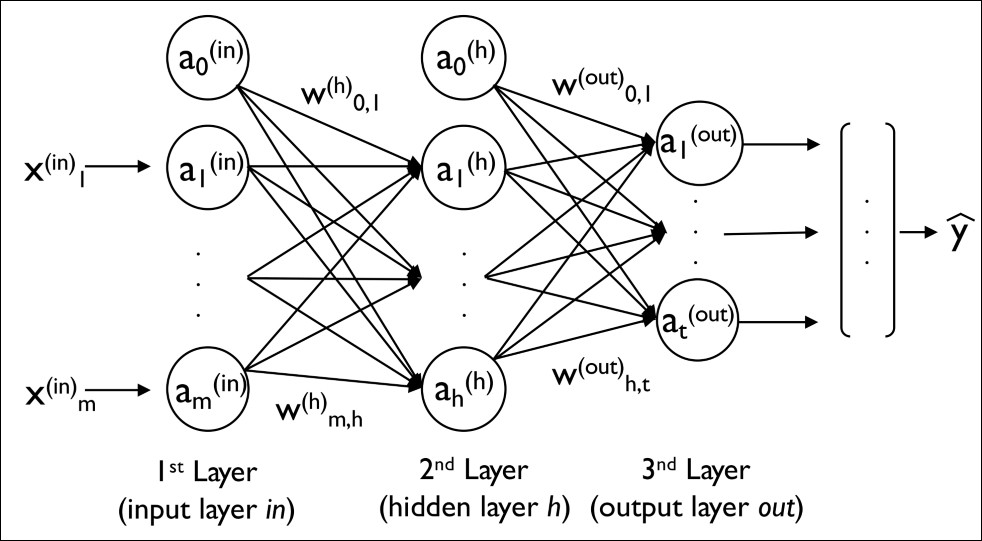
\includegraphics[width=0.6\columnwidth]{figures/MLP.jpeg}
        % note that in above figure file name, "sr_setup",
        % the file extension is missing. LaTeX is smart enough to find
        % apropriate one (i.e. pdf, png, etc.)
        % You can add this extention yourself as it seen below
        % both notations are correct but above has more flexibility
        %\includegraphics[width=1.0\columnwidth]{sr_setup.pdf}
        \caption{
                \label{fig:mlp} % spaces are big no-no withing labels
                % things like fig: are optional in the label but it helps
                % to orient yourself when you have multiple figures,
                % equations and tables
                An example of a MLP, taken from \cite{newmlp}. In this example, predictions $\hat{y}$ are generated from inputs $x^{(in)}$ using artificial neurons $a$ and weights $w$.
        }
\end{figure}

Whilst it is possible to train these MLPs with the Hillas parameters for a set of IACT images (though they tend to be inferior classifiers to BDT methods due to the fact that they don't prioritise parameters based on separation power \cite{hessbdt}), 
using every pixel value of an image as an input to an MLP tends to be computationally prohibitive.

\subsection{Loss Functions and Metrics}
\label{MLdefs}
In order to train a neural network, one needs to define a loss function for the training algorithm to optimise against. For binary, two class classification, the appropriate choice for this is the  binary cross entropy (BE) between the actual known classes $t_i$ and the score assigned by the network for an event having that class $s_i$ \cite{Keras}. This is defined over $N$ events as
\begin{equation}
    \textrm{BE}=-\frac{1}{N}\sum_{i=1}^{N}t_i\ln{s_i}+(1-t_i)\ln{(1-s_i)}.
\end{equation}

For multi-class (>2) classification the most appropriate choice is a \textbf{Categorical Cross-Entropy Loss Function (CE)}. This is defined \cite{Keras} as :
\begin{equation}
    \textrm{CE}=-\sum_i^N \ln \left( \frac{e^{t_{i}}}{\sum_j^3 e^{s_{ij}}} \right)
\end{equation}

where there are N events, $s_{ij}$  is the CNN score for each of the possible event classes for the event $i$ and $t_{i}$ is the CNN score for the target (true) class for that event. This equation relies on the CNN input labels being `one-hot' encoded such that the label for class $0$ is represented as $[1,0,...]$, class $1$ as $[0,1,...]$ so on \cite{fb}. In practice, during the training of the ConvLSTM2D network results in chapters \ref{ch:3-TimingInfo} and \ref{ch:4-VERITASRealData}, there is an additional regularization penalty added to the total loss used due to the L2 regularization we use in the first two ConvLSTM2D layers. This regularization is designed to prevent network weights from taking extreme values.

\begin{table}[ht]
    \centering
    \resizebox{0.7\textwidth}{!}{
    \begin{tabular}{c|c}
    \textbf{Term} & \textbf{Definition}\\
    \hline
    \textbf{True Positive (TP)} & True Label Positive and Classification Positive\\
    \textbf{True Negative (TN)} & True Label Negative and Classification Negative\\
    \textbf{False Positive (FP)} & True Label Negative and Classified Positive\\
    \textbf{False Negative (FN)}& True Label Positive and Classified Negative\\
    \end{tabular}  
    }
    \caption{Definitions of Event Classifications for binary classification, taken from \cite{fawcett}.}
    \label{table:FPR}
\end{table}

For the purposes of evaluation of network performance, \textbf{Categorical Accuracy} \cite{Keras} is defined as the percentage of events for which the \textit{Argmax} of the one-hot-encoded predicted label is the same as the \textit{Argmax} for the one-hot-encoded true label (the definition of binary accuracy is similar for 2-class classification \cite{Keras}). Given the definitions for binary classification in Table \ref{table:FPR}, the \textbf{True Positive Rate (TPR)} and \textbf{False Negative Rate (FNR)} are defined by \cite{fawcett}:
\begin{equation}
    TPR=\sum_{Events}\frac{TP}{TP+FN}=1-FNR
\end{equation}
and the \textbf{True Negative Rate (TNR)} and \textbf{False Positive Rate (FPR)} by
\begin{equation}
    TNR=\sum_{Events}\frac{TN}{TN+FP}=1-FPR.
\end{equation} For multi-class ($>2$ class) classification, such as in Chapter \ref{ch:3-TimingInfo}, we use a one-versus-all approach where for each individual class the classifications are treated in a binary way (such as $\gamma$-ray or not-$\gamma$-ray) \cite{fawcett}\cite{scikit}. 

\subsection{Universal Approximation Theory}
Universal functional theory states that a neural network can be made to replicate the behaviour of any function, provided sufficient training data exists. However in practice this is limited by finite training data, a finite number of neurons in a layer, and a finite number of layers \cite{universal}. Ultimately through training for IACT event classification, it is such a function that we wish CNN-based classifiers to replicate, mapping a set of input images to an output event score. 

\subsection{Activation Functions}

The summed inputs to an artificial neuron are evaluated against activation functions. This is crucial to neural networks being able to solve highly non-linear problems such as the EXOR problem \cite{universal}. In particular, the final layer activation function in a neural network determines the form of the neural network output. The precise mathematical form of the activation function used by the neuron is a choice for the user; the earliest neural networks used simple Heaviside Step functions, but 
it is common to use Linear Rectifier (ReLU), $\tanh$ ($\sigma_T$) or sigmoid ($\sigma_S$) functions as they are useful for analysing nonlinear relationships \cite{C++CNN}\cite{Keras}. 

The Linear Rectifier Function ($\textrm{ReLu}(x)$) as a function of input variable $x$ as a function of threshold variable $y$ (typically 0, but configurable) is defined by
\begin{equation}
    \textrm{ReLu}(x)=\begin{cases}\mbox{0} & \mbox{, if } x <= y \\ \mbox{x} & \mbox{, otherwise} \end{cases}
\end{equation}

\cite{Keras}. The Sigmoid function ($\sigma(x)$), appropriate as the final layer activation function for binary classification. It takes the form

\begin{equation}
    \sigma(x)=\frac{1}{1+\exp(-x)}
\end{equation}

The Softmax function is a generalization of the Sigmoid function, and is appropriate as the final layer activation function for multi-class (>2 class) classification. For a vector input $(\textbf{x})$ with $i$th components $x_i $ and a given number of classes $K$ it is defined as
\begin{equation}
    \sigma(\textbf{x})_i=\frac{e^{x_i}}{\sum_{j=1}^K e^{x_j}}
\end{equation}

Neural networks can also be used as a method for regression, by having training data with continuous labels and modifying the activation function of the final layer in the network to provide a score on a continuous space. This can be used for IACTs for directional and energy reconstruction, however this thesis doesn't approach this issue (further information can be found for example in \cite{mikaelphd}, \cite{tjarkicrc}).  

\subsection{Convolutional Neural Networks}
Convolutional Neural Networks (CNNs) are a type of neural network developed specifically to handle image data, inspired by the mechanics of the visual cortex in the brain. Although the concept of a CNN dates back to 1980 (the so called neocognitron \cite{neocongnitron}), the first modern use of this taking advantage of GPU power was in a paper by Ciregan et.al. in 2012 \cite{ciregan}. CNNs take advantage of two properties of images, the translational invariance of useful data in the image (i.e. in Figure \ref{fig:carnet} it doesn't matter where in the image the car is located for the image to be classified as containing a car) and the relative sparsity of useful information in the image (i.e. the network does not need a million pixels to detect the presence of a tyre). The CNN achieves this in a `convolutional layer' by only feeding a few neighbouring pixels (a so-called receptive field) into each neuron, which are arranged in a 2D grid. The weights of these neurons are then shared throughout the convolutional layer in order to achieve the effect of translational invariance. Through pooling, downsampling and flattening, 
these neurons feed into MLP-like layers at the end of the network to perform a classification. CNNs are a promising technology for CTA analysis, as the entirety of the information contained in an IACT image can be used.  Another key advantage such CNN-based methods is the speed at which they can perform classifications of complete images (approximately 1kHz for Mono-telescope analysis using a NVidia 1080Ti GPU), which is a major factor to consider given the high expected array trigger rate of CTA (approximately 10 kHz for a full CTA array [56], although this estimate requires updating for the 'alpha' array configuration).

\begin{figure}[t!] 
        % read manual to see what [ht] means and for other possible options
        \centering 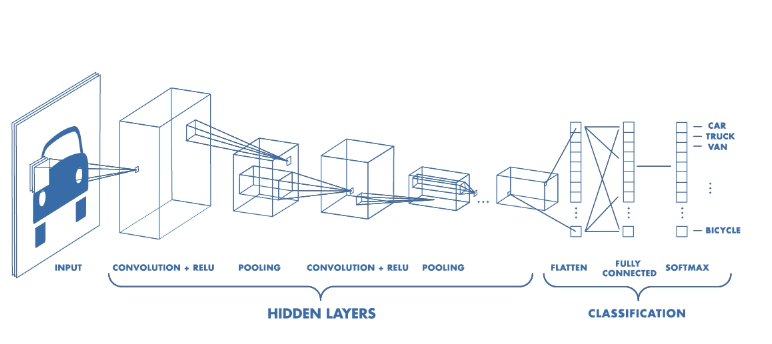
\includegraphics[width=1.0\columnwidth]{figures/carnet.png}
        % note that in above figure file name, "sr_setup",
        % the file extension is missing. LaTeX is smart enough to find
        % apropriate one (i.e. pdf, png, etc.)
        % You can add this extention yourself as it seen below
        % both notations are correct but above has more flexibility
        %\includegraphics[width=1.0\columnwidth]{sr_setup.pdf}
        \caption{
                \label{fig:carnet} % spaces are big no-no withing labels
                % things like fig: are optional in the label but it helps
                % to orient yourself when you have multiple figures,
                % equations and tables
                An example of a CNN, taken from \cite{mathworks}. Images are fed into convolutional layers, the outputs of which are flattened and fed into a MLP-like network prior to the output layer. Increasing the number of layers (depth) of the network increases the abstraction of the features recognised.
        }
\end{figure}
\subsection{Long Short-Term Memory Networks and ConvLSTMs}

Long Short-Term Memory networks (LSTMs) are are an established form of neural networks for time series analysis (which are more generally known as Recurrent Neural Networks or RNNs). They are heavily used in industry for classification tasks which require the ability to handle input vectors of varying length and having varying time intervals between useful information. A classic example of such a task is speech recognition.
LSTMs are mathematically similar to MLPs, except that the neurons are arranged such that there are loops in the network architecture, and the individual cells within the network contain vectors $\textit{c}$ to act as a memory as well as a function to `forget' elements from that memory $\textit{f}$, an input function $\textit{i}(x)$ and an output function $\textit{o}$ that produces an output vector $O_t$ at a timestep $t$. The equations used in the initial paper on LSTMs define a forward pass through a cell \cite{Hochreiter} as
\begin{align}
\begin{split}
\textit{f}_t &= \sigma_s(W_{f} x_t + O_{f} h_{t-1} + b_f) \\
\textit{i}_t &= \sigma_s(W_{i} x_t + O_{i} h_{t-1} + b_i) \\
\textit{o}_t &= \sigma_s(W_{o} x_t + O_{o} h_{t-1} + b_o) \\
\textit{c}_t &= \textit{f}_t \circ c_{t-1} + \textit{i}_t \circ \sigma_t(W_{c} x_t + U_{c} O_{t-1} + b_c) \\
O_t &= o_t \circ \sigma_t(\textit{c}_t)
\end{split}
\end{align}
where $\circ$ is an element wise product, $U$ is an additional weight matrix, and finally $b$ are bias vectors which must be trained. It is also possible to combine the properties of LSTMs and CNNs together to form ConvLSTMs, the 2D versions of which are ideal for classifying time sequences of images from IACTs. These ConvLSTMs are similar in structure to conventional LSTMs, but their internal matrix operations are replaced by convolutional operations. 
\begin{figure}[ht] 
        % read manual to see what [ht] means and for other possible options
        \centering 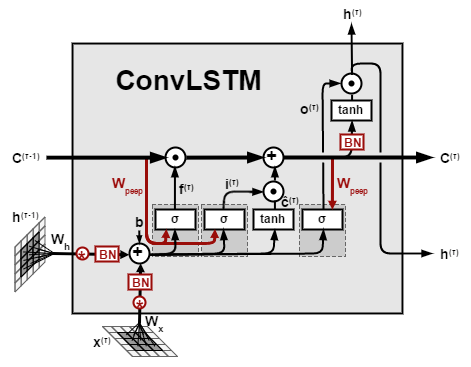
\includegraphics[width=0.5\columnwidth]{figures/convlstmcell.png}
        % note that in above figure file name, "sr_setup",
        % the file extension is missing. LaTeX is smart enough to find
        % apropriate one (i.e. pdf, png, etc.)
        % You can add this extention yourself as it seen below
        % both notations are correct but above has more flexibility
        %\includegraphics[width=1.0\columnwidth]{sr_setup.pdf}
        \caption{
                \label{fig:convlstmcell} % spaces are big no-no withing labels
                % things like fig: are optional in the label but it helps
                % to orient yourself when you have multiple figures,
                % equations and tables
                An illustration of the architecture of a ConvLSTM cell, taken from \cite{convlstmintro}
        }
\end{figure}
A more detailed comparison between our ConvLSTM approach and the existing CRNN approach from Shilon et. al \cite{Shilon} can be found in Chapter \ref{ch:3-TimingInfo}.

LSTMs have now largely been supplanted by methods based on \textit{Attention} (a form of trainable weighted sum applied using fully connected dense layers in parallel) for most common time series analysis in industry. The \textit{CTLearn} \cite{tjarkicrc} CTA deep learning event reconstruction framework now offers a hybrid CNN/attention scheme, although the benefit of this for IACT analysis (compared to conventional CRNN methods) is currently unclear.

\subsection{Hyperparameters}
All machine learning algorithms (more complex than linear regression) have some number of hyperparameters, user-configurable options that define their architecture and the process of their optimisation. As examples, for a BDT or RF, this can be the number of trees in the classifier ensemble or the rate of `pruning' (the removal of branches from the trees), and for neural networks these can be the number of artificial neurons/convolutional filters per layer. Deep learning analyses innately require a greater number of hyperparameters than their conventional counterparts \cite{hyperopt}. Setting the values for these hyperparameters has typically been something of a dark art, although automated methods for determining hyperparameters have been developed \cite{hyperopt}. We explore this further in chapters \ref{ch:3-TimingInfo} and \ref{ch:4-VERITASRealData}.

\subsection{Weight Optimisation Algorithms}
The choice of weight optimiser used during training is also an example of a hyperparameter. Various algorithms exist to optimise the weights in a neural network during training. In Chapter \ref{ch:3-TimingInfo} we use the Adadelta algorithm to optimise our ConvLSTM2Ds as this was the \textit{Keras} recommended choice \cite{adadelta}, in Chapter \ref{ch:4-VERITASRealData} we found the Adam optimiser \cite{adam} performed marginally better.

Crucial to the performance of these algorithms is the concept of Backpropagation, which in effect allows the neural network optimiser to predict the effect of a change in a layer's weights by using the chain rule to compute a gradient (and therefore examine the effect of changing weights) in the loss function. Virtually all neural network optimisation algorithms use this technique \cite{goodfellow2016deep}.

\subsection{Over- and Under-training}
\begin{figure}[ht] 
        % read manual to see what [ht] means and for other possible options
        \centering 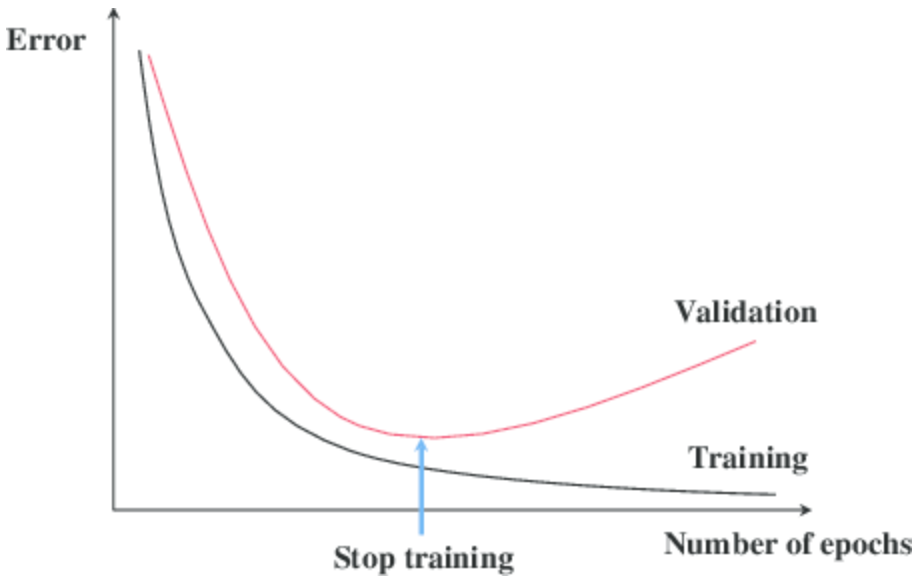
\includegraphics[width=0.7\columnwidth]{figures/overtrain.png}
        % note that in above figure file name, "sr_setup",
        % the file extension is missing. LaTeX is smart enough to find
        % apropriate one (i.e. pdf, png, etc.)
        % You can add this extention yourself as it seen below
        % both notations are correct but above has more flexibility
        %\includegraphics[width=1.0\columnwidth]{sr_setup.pdf}
        \caption{
                \label{fig:earlystop} % spaces are big no-no withing labels
                % things like fig: are optional in the label but it helps
                % to orient yourself when you have multiple figures,
                % equations and tables
                An illustration of the concept of over and under training, where error here can be considered equivalent to loss, taken from \cite{earlystop}, in practice we found the use of validation data to be unreliable and highly noisy.
        }
\end{figure}

Neural networks can be both over- and under- optimised during the training process, a feature illustrated in Figure \ref{fig:earlystop}. One option to prevent this is to define an early stopping condition, whereby training is abandoned and the weights in a network reverted to those from a previous epoch, though this depends on both reliable validation performance and the ability to define a suitable metric by which to stop training. We encounter such issues in Chapter \ref{ch:3-TimingInfo}.


\subsection{Dropout and Regularization}
Dropout refers to a procedure during training of randomly setting weights in the network to zero, at a configurable rate. This is an extremely common practice in deep learning and is designed to prevent overtraining of networks. Typically, the dropped out weights are frozen after training, but applying dropout during testing can be used as a method of pseudo-simulating Bayesian posteriors \cite{mike}\cite{gal2015}. 

Regularization is a similar technique whereby additional bias terms are introduced to neural network loss functions to penalize overly-large weights, and thus also prevent overtraining. In this work, we use L2 regularization whereby a quantity ($L2$) defined by
\begin{equation}
    L2=\lambda\sum_{i}w_i^2
\end{equation}
, where $\lambda$ is a configurable hyperparameter and $w_i$ are the network weights, is added to the loss function \cite{Keras}.

In the \textit{Keras} \cite{Keras} package, dropout and regularization can be applied to the CNN elements of a network (Kernel Dropout and Regularization) or the Recurrent elements of a network (Recurrent Dropout and Regularization) or both; the rate and $\lambda$ terms of both being configurable hyperparameters.

\section{Past and Concurrent Work on CNN Use With IACT data}
In this section, we review recent relevant work concerning the use of these new machine learning methods for IACTs.

\subsection{Muon Tagging and Muon-Hunters}
The first published work to consider the potential for CNN-type analysis with IACTs was Feng et.al in 2016 \cite{feng2016}, in which they consider the use of CNNs for muon ring classification (selecting events where a muon has passed directly down the optical path of an IACT and has therefore produced a characteristic 'ring' image) as well as muon ring radius/size regression with VERITAS. By measuring the width and detected Cherenkov light intensity of such events, one can infer the efficiency of the IACT's optics. VERITAS has also investigated the use of active learning for the same purpose through the Muon Hunters 2.0 project \cite{muonhunters2}, whereby classifications from citizen scientists are used in combination with Bayesian deep learning to improve classifications.

Whilst active-learning is an extremely interesting area of computer science research, and an excellent opportunity to engage the public, the task of gamma/hadron separation for CTA is less well suited for active-learning-type analyses for a number of reasons. Firstly, the likely trigger rates \cite{trigrate} of CTA are probably beyond the reasonable capacity of an active-learning pipeline, as the number of citizen scientist volunteers over time is usually approximately constant. Secondly, current active-learning analyses can have significant biases inherited from the intuition of volunteers (such as the redshift dependence on galaxy morphology classification in \cite{mike}), that are probably currently intolerable for high level scientific analysis to be reliably performed. Thirdly, gamma/hadron separation for IACTs is both a subtle (relying on small differences between images and therefore difficult for humans to perform) and uninteresting task. There are likely no exciting discoveries, equivalent to new types of Galaxy or new planets, for citizen scientist volunteers to make in IACT event classification images that could not be simply detected in IACT data by (for example) selecting the brightest (highest energy) events. Bandwidth is also an issue, it is unlikely we will be able to get all IACT images for all CTA instruments off the southern CTA site, some degree of online data processing will likely be necessary. Finally, these active-learning analyses are fundamentally vulnerable to the same run-by-run experimental variations as CNNs, which we discuss later Chapter \ref{ch:4-VERITASRealData}. As such, supervised machine learning methods remain the most promising for IACT event classification.

R. Clark has also recently studied further potential options for muon tagging with CHEC-S and ASTRI simulated data using CNNs \cite{roganthesis}, particularly concerning the tagging of partial muon rings against proton EAS background. Whilst he found that CNNs can identify partial muon rings (despite the complexity of generating a simulated dataset suitable for this analysis), it appears as if using supervised CNNs for online muon tagging will suffer many of the same issues surrounding CNN use for IACT background rejection that we explore further in Chapter \ref{ch:4-VERITASRealData}.

\subsection{Work of Shilon et al. and Parsons et al.}
Shilon et al. \cite{Shilon} and Parsons et al. \cite{ParsonsOhm} are the two papers currently in press that concern the application of deep learning event reconstruction methods to H.E.S.S. data. Whilst these have provided significant advances in the field (particularly in the case of the Shilon et al. work), there are a number of underlying issues that have become apparent since their publication.

In the Shilon et al. work \cite{Shilon}, the authors feed images from the CT1-4 telescopes into convolutional layers that then feed into an LSTM Network. This technique, called the Convolutional Recurrent Neural Network (CRNN) method, treats the set of four charge images from the four IACTs as a time series. The authors of the Shilon et al. work justify this network architecture using the assumption that that the images with the largest size parameter (total charge) are those closest to the shower core, and that this ordering compensates for the lack of available temporal information in their case \cite{Shilon}. Using this, they observed performance in background rejection superior to the current BDT paradigm with simulations, and were able to perform a significant detection of PKS 2155-304 with real observations. The CRNN technique achieved a 50.8$\sigma$ detection with this data relative to a BDT which achieved 46.1$\sigma$, though the statistical significance of this difference has not been completely explored. In particular, this source is extremely bright, and so this data is likely $\gamma$-dominated. Whilst this network architecture allowed for the first CNN-based detection of an astrophysical source, the Shilon et al. work's authors' assumption that the ordering of the images in the LSTM is significant has not necessarily held up to subsequent scrutiny, with other charge image orderings \cite{ariconf} being seen to provide equivalent or superior performance. As a result, for the purposes of our work in later chapters, we treat the LSTM-type features in similar networks as a computational tool. Whilst this tool is useful for avoiding the need to stack images from multiple telescopes into single images in order to apply CNN-type analyses (which had been the standard previous to the Shilon et al. work and doesn't scale well in the case of multiple IACTs \cite{Shilon}\cite{salvatore} as details in images from high multiplicity events is lost), we ultimately don't assume the use of the LSTM features in such networks to be of further physical significance in later chapters. Additionally, the Shilon et al. paper considers directional reconstruction, however the directional and gamma/hadron separation elements of the paper are applied to differing flaring states of PKS2155-304, suggesting significant issues with applying stereoscopic directional reconstruction methods to real observations. The most likely cause of this is a lack of an appropriate pointing correction algorithm for CNN-type analysis and the difficulty of taking appropriate account of IACT positions on the ground. The later Parsons et al \cite{ParsonsOhm} work attempts to hybridise CNN-type methods with parametric inputs such as impact parameters for background rejection, however this defeats part of the point of using whole-image CNN methods. Ideally, the aim is to get the CNN classifier to learn image features related to (for example) impact distance from the images themselves. It is also not at all clear in that paper the relative contributions of the image and parametric network components to the event classification, a parametric MLP with the same parameterised data would likely perform as well as the hybridised CNN approach. It is not currently clear how well these CNN-based event classification methods will work with dimmer sources given their high level of sensitivity to small differences between real observations and simulations. We explore such issues related to real observations further in Chapter \ref{ch:4-VERITASRealData}.

One critical issue that both the Shilon et al. and Parsons et al. paper share is their reliance on tailcut cleaning of images prior to deep learning analysis. For example, see the following quote from the Shilon et al. paper:
\begin{quote}
    \textit{The raw simulated images are cleaned according to the standard H.E.S.S. cleaning scheme.}
\end{quote}

The complication from this is that if the aim of deep-learning-based event classification methods on photomultiplier charge data is to improve sensitivity to subtle features in IACT images, tailcut cleaning will make analysis of real observations simpler (as only a handful of pixels' noise needs to be accurately modelled rather than several hundred), but will remove the features in the images we aim to exploit. Whilst this can be argued as being a necessary constraint of a proof-of-concept study (common in many astronomy deep learning papers, see for example \cite{dodgygal}), in the long run if deep learning event classifiers cannot be performed without tailcut image cleaning they will never pass a cost/benefit analysis, and as such we should aim to find ways of avoiding the need to do so. However, performing tailcut image cleaning before directional reconstruction is more tolerable, given that there is less need to examine small features around the edge of the shower image. We explore the limitations of performing charge-based deep learning event classification, without tailcut image cleaning, in Chapter \ref{ch:4-VERITASRealData}.  

\subsection{Full Event Reconstruction and Instrument Response Functions}
For most of the time the research performed in Chapter \ref{ch:3-TimingInfo}, a Python-based method of generating Effective Areas, Angular Resolution plots and Energy Sensitivities, examples of Instrument Response Functions (IRFs), based on ctapipe and its associated pipelines did not exist. At the time of writing this is now only partially the case, and prototype methods of performing this have yet to undergo a monte-carlo validation effort for either CHEC-S or SSTCAM (and currently produce inferior results to those generated with \textit{Eventdisplay}). Much of the current work of the CTA task force on machine learning now focuses on generating these instrument response functions with deep learning classifiers, directional reconstructors and energy reconstructors \cite{tjarkicrc}. However, fundamentally the underlying task of CNN-based reconstruction has not changed, despite the ability to generate these new results. Additionally given the real observations issues explored in the next section, such IRFs generated using these pipelines likely have difficult to quantify systematic errors associated with the discrepancies between real and simulated data, as well as having issues with gammaness cut optimisation and asymmetric posteriors for gammaness \cite{mike}. As such, IRFs based on deep learning analyses pipelines may well be unreliable in practice for the foreseeable future. We explore these issues in depth in later chapters.

\subsection{Multi-Task Learning}

One option is to design a CNN-based architecture to perform the tasks of event classification, directional reconstruction and energy reconstruction simultaneously, work currently being done by the \textit{Gammalearn} project \cite{mikaelphd} (primarily for single telescope analysis). The motiviation for this is that there are physical correlations between the event impact distance and apparent energy. Whilst a very interesting area of investigation, attempting to perform multiple IACT analysis tasks simultaneously makes it difficult in practice to discern where any improvement in performance originates from, and it also makes the implicit assumption that the optimal simulation and analysis setup is the same for Event Classification, Directional Reconstruction and Energy Reconstruction. This is not mandated to be the case, in all likelihood given the existence of ImPACT, the main potential benefit from deep-learning-based directional reconstruction is speed, whereas for gamma-hadron separation the main goal is likely to be sensitivity. Similarly, applying tailcut cleaning for $\gamma$/hadron separation with deep learning classifiers largely defeats the purpose of using whole image analysis, whereas tailcut cleaning for directional reconstruction is more likely to be tolerable (and will help against NSB) since there is less dependence on minute features near the shower image edge. That said, the clear sensitivity of CNNs to event direction we find in Chapter \ref{ch:3-TimingInfo} suggests there may be a significant benefit to performing event classification and directional reconstruction simultaneously.

\section{Known Issues with CNN-Type Analysis Techniques}
In the following subsections we discuss the various known issues associated with the use of CNNs for CTA analysis. It is helpful to define problems when exploring new analysis methods as it helps in the process of defining goals and limitations. This is particularly true in the case of CTA, as it consists of a new set of instruments with new procedures and analysis requirements,

\subsection{The Camera Geometry Problem}

Firstly, CNNs are primarily designed to process square images. This creates an issue for using CNNs with CTA data as many of the camera prototypes have focal planes which are either hexagonal or have regions without photodetectors (like CHEC, which doesn't have photodetectors in its corners). In the case of hexagonal cameras, there are two options to avoid the risk of geometric bias. The first is to resample or oversample the hexagonal image in order to make it square, this is the approach taken in a paper by Holch et.al. \cite{Hexagdly} and used in Chapter \ref{ch:4-VERITASRealData} for our VERITAS data. The second option is to write a custom CNN code that can handle hexagonal images based on computing convolutions based on nearest neighbour information, which may also be applicable to CHEC/SSTCAM (in the analysis in Chapter \ref{ch:3-TimingInfo} we just crop images to the square central region of the camera). The disadvantage of this custom CNN approach is that it limits the potential for more sophisticated network architectures, and at present has not been extended to stereoscopic analysis. Graph-based Chebyshev networks \cite{adithesis} might provide an alternative solution to this problem in the long term, as they only require that an adjacency matrix can be defined for the camera plane, as opposed to having to perform transformations to place the IACT images on a Euclidean grid. 

\subsection{The Multiple Telescope Problem}

CTA will operate stereoscopically, and combining images from multiple telescopes (separated by varying distances on the ground and differing impact distances) to use with CNNs is a problem unique to IACTs. The simplest method of solving this problem used by many IACT researchers is to simply add the pixel values from the various telescopes together and feed this single image to a CNN \cite{mangano}. The problem with this is that it doesn't take account of the telescopes' positions on the ground, which is an issue for performing accurate reconstruction. It also doesn't scale well to large arrays; if only five telescopes are triggered in an array of a hundred, the resulting stacked images are very sparse (a problem for CNNs). This is complicated further by CTA's multiple classes of telescope.

Over the course of the investigations included in chapters \ref{ch:3-TimingInfo} and \ref{ch:4-VERITASRealData}, it has become apparent that there will likely always be some degree of tension between the most advanced deep learning analyses possible and stereoscopic IACT analysis. This is as single image analysis is both a more common task and is easier to perform.  However it is important to note that stereoscopic analysis for IACTs basically always achieves superior sensitivity and event angular resolution against single image analysis with any analysis method, as the pixel density and effective area of a single IACT is limited by technological constraints. As such, if deep learning analysis cannot eventually work on images from multiple IACTs, it no longer becomes worth investigating in the context of an advanced analysis method for CTA.

As of the time of writing, no CTA deep learning analysis study has seriously considered the prospect of deep learning event classification with multiple classes of CTA telescope observing the same event. This may be one of the must crucial avenues of investigation given the flexibility deep learning offers in considering partially truncated shower images. However, investigating this comes with significant computational cost and simulation complexity.

\subsection{The Hyperparameter Problem}
CNN-type methods require a large number of hyperparameters, which aren't trivial to human-interpret. The optimal combinations of these for IACT data may be a function of instrument observational energy, plate scale and observation conditions, and automated optimisation strategies for these are highly computationally costly. Additionally hyperparameter selection can have an effect on training convergence, which makes comparison of differing models complex. We explore these issues in depth in Chapter \ref{ch:4-VERITASRealData}.

\subsection{The Real Observation Problem}
Whilst one of their greatest strengths, the fact that CNNs are sensitive to minute morphological features in their training datasets can also present significant issues. The most troublesome problem arises from the fact that we need a labeled input dataset in order to train our networks. In certain cases (such as transient searches\cite{SNH}) this dataset can be produced from real observations by hand, or through the involvement of citizen scientists. However, for the purpose of CTA image analysis this is not possible. As a result, we are forced to train our neural networks on data simulated using Monte-Carlo simulations for which we know the 'true' event parameters, and then use these trained networks to analyse real observations. The slightest discrepancy between the real and simulated data (for example from night sky background, optical efficiency losses due to the ageing of the telescopes or imperfect calibration) has the potential to affect the resulting analysis. One particular source of concern for the CTA SSTs in particular is the uncertainty in modelling hadronic processes at high energies (notably in the CTA standard \textit{Quark Gluon String with JETs (QGSJet)} package used by \textit{CORSIKA}), due to a lack of forward momentum data from the LHC. Significant work to improve these models is nonetheless underway \cite{hadronmodel}.

One potential solution to this problem has been proposed by Erdmann et.al. \cite{ErdmannAuger}. Their suggestion is the use of Generative Adversarial Networks, which are essentially two CNNs playing off each other in a zero sum game \cite{goodfellow2016deep}, to perform an intelligent, machine learning based correction to simulated data such that it resembles real observations more closely for the purpose of training a CNN. We briefly further discuss the potential applications of GANs in chapters \ref{ch:3-TimingInfo} and \ref{ch6-Conclusions}.

\subsection{The Class Imbalance Problem}

Not every $\gamma$-ray source on the sky is equally bright, and so real test data will typically be imbalanced (i.e. not have a 50:50 $\gamma$ to proton ratio). In certain IACT use cases, such as obtaining dark matter annihilation constraints from observations of dwarf spheroidal galaxies (such as \cite{gloryduck}), the observational data will be proton dominated. In particular, this is complicated by trigger selection. As a result, there is a need for a future detailed investigation into the effects of using more realistic, imbalanced training data with CNN-type IACT background rejection methods, as such imbalanced datasets require specialised deep learning treatments \cite{imbalance}.

\subsection{The GPU Cost and Availability Problem}
Without access to high-performance GPUs, deep learning analysis would be prohibitively slow an analysis method for CTA at both training and inference times. Whilst extremely powerful computational tools, GPUs are very expensive \cite{gpucost}, in very short supply \cite{gpushort}, power hungry \cite{2080ti} and thus costly to run \cite{2080ti}. These practical considerations must be taken into account when considering deep learning as a potential general analysis method for CTA. In the long term, and broadly speaking for the majority of analyses, deep learning analysis must have a reasonable prospect of passing a cost/benefit analysis whereby if deep learning offers a 10\% improvement in sensitivity, it must be less than 10\% more computationally and financially costly compared to conventional analysis. At the time of writing, this is nowhere near the case, however there could be specific analysis cases where such costly analysis methods could be justified if it opens the potential for new physics (such as looking for dark matter annihilation constraints through observing dwarf spheroidal galaxies\cite{gloryduck}).

Given these issues of availability and cost, there is a serious risk of deep-learning-based research in the physical sciences becoming a 'walled garden', whereby only the richest or most cited researchers have access to sufficient compute power to perform state-of-the-art deep learning analyses \cite{gpudivide}. Ideally, GPU time should be allocated based on scientific merit, and to their credit the UK's Science and Technology Facilities Council (STFC) are now providing such a peer reviewed resource through their iris scheme, now being utilised by CTA.
\chapter{\label{ch:3-TimingInfo} Use of Timing Information In Combination With Deep Learning as an Event Classifier for SSTCAM}

\minitoc

\begin{abstract}
%% Text of abstract
New deep learning techniques present promising new analysis methods for Imaging Atmospheric Cherenkov Telescopes (IACTs) such as the upcoming Cherenkov Telescope Array (CTA). In particular, the use of Convolutional Neural Networks (CNNs) could provide a direct event classification method that uses the entire information contained within the Cherenkov shower image, bypassing the need to Hillas parameterise the image and allowing fast processing of the data. 

Existing work in this field has utilised images of the integrated charge from IACT camera photomultipliers, however the majority of current and upcoming generation IACT cameras have the capacity to read out the entire photosensor waveform following a trigger. As the arrival times of Cherenkov photons from Extensive Air Showers (EAS) at the camera plane are dependent upon the altitude of their emission and the impact distance from the telescope, these waveforms contain information potentially useful for IACT event classification. 

In this test-of-concept simulation study, we investigate the potential for using these camera pixel waveforms with new deep learning techniques as a background rejection method, against both proton and electron induced EAS. We find that a means of utilising their information is to create a set of seven additional 2-dimensional pixel maps of waveform parameters, to be fed into the machine learning algorithm along with the integrated charge image. Whilst we ultimately find that the only classification power against electrons is based upon event direction, methods based upon timing information appear to out-perform similar charge based methods for gamma/hadron separation. We also review existing methods of event classifications using a combination of deep learning and timing information in other astroparticle physics experiments.
\end{abstract}

%% \linenumbers

%% main text
\section{Introduction} \label{Introduction}

We present in this chapter the first work to consider applications of 2-Dimensional Convolutional Long Short-Term Memory (ConvLSTM2D) Networks techniques in the high energy range probed by the SSTs. The significance of this approach lies in the fact that not all EAS are caused by $\gamma$-ray photons, and background rejection is a key component in IACT sensitivity \cite{Shilon}. This work is the first known attempt to determine if new deep learning techniques and new prototype instruments have any potential to aid in discriminating against cosmic-ray electrons using a combination of complete images and photosensor waveform data, suggested as a possibility by Nieto et. al in \cite{nieto2017exploring}. Previous (largely unsuccessful) attempts at the highly challenging task of $\gamma$-electron event separation for IACTs have relied upon indirect estimation of first interaction height from IACT images using either shower image shape or combined shower energy and maximum estimation \cite{Sitarek1i}.

We split the main body of this chapter into five sections. In section 2, we discuss recent advances in machine learning techniques in astroparticle physics, particularly concerning the use of timing information in combination with deep learning techniques as a background rejection method. In section 3 we detail the simulated datasets we use and in section 4 we describe the analysis we perform. In section 5 we present our results and we conclude in section 6. 

\section{Timing Information as an Event Classification Method in Other Experiments} \label{RelatedWork}

The use of EAS timing information for event classification in IACT data has been considered as early as in \cite{paulathesis}. More recently, it has been used as an image cleaning method on MAGIC (whereby pixels associated with Cherenkov light are partly selected based upon photon arrival time) \cite{magictime}, prior to their RF analysis. Similar studies to this have also been performed with VERITAS \cite{jamietime}. MAGIC also use parametric timing data such as a time gradient (how fast the arrival time changes along the major IACT image axis) and Time RMS (the RMS arrival time of photons to all pixels that survive an image cleaning process) as part of their RF-based background rejection method \cite{supermagictime}. In that work \cite{supermagictime}, the MAGIC collaboration also demonstrate the dependency of timing structure upon the impact parameter of the shower, also information useful for background rejection. The attraction of deep learning in our use case is the ability to use this timing information for background rejection directly, in addition to the other pixel-wise data (such as evidence of electromagnetic shower sub-structure in hadronic showers), without the need for parameterisation. An illustration of this information can be seen in Figure \ref{fig:wfplot}. Whilst this is the first work to attempt such a combination of timing information and deep learning for IACTs, this is not the case for other air shower experiments, and so in the remainder of this section we investigate the approaches taken by other groups.

Erdmann et al. \cite{aug1} investigated the use of deep learning to perform energy and angular event reconstruction of air showers for a model hexagonal array of 81 ground based water Cherenkov detectors using a custom simulation code. They feed in waveforms from their array into a CNN, which is concatenated with 2D feature maps of the first particle arrival time and integrated charge for the entire detector grid approximately half way through their network architecture. These feature maps are then treated with separable convolutions, as it is not expected that the correlations between the feature maps will be coupled to spatial correlations within the maps themselves. The use of this information allows them to achieve an energy resolution of 5\% in the EeV energy range, compared to 8\% without the additional concatenated feature maps. We do not attempt a similar approach here (as has recently been attempted as an expansion to the Shilon et al. work by \cite{ParsonsOhm}) as it becomes even more difficult to interpret the behaviour of the neural network when parameterised data (such as impact parameters) is mixed with image data. In a later paper \cite{ErdmannAuger}, the authors investigate their analysis robustness to real data effects by creating air shower simulation datasets with different divisions of energy between the muonic and electromagnetic components of the showers. They successfully train a 1-dimensional Generative Adversarial Network (GAN) in order to attempt to refine their 1-dimensional waveform traces from one simulation set such that it resembles the second set of simulations more closely. This is an attempt to handle the problem that minute differences between training and test sets in machine learning analyses can cause discrepancies; however they find that the differences between their simulated datasets are insufficiently large to affect their quality of the energy reconstruction. However, 2D image data is substantially more complex and it is unclear how well a GAN would perform in our case. A study has also been performed on data from the Tunka-Rex experiment \cite{tunka} on 1-dimensional timing information regarding the radio emission from $>100$ PeV air showers which provided improved background suppression, however this was only performed on single traces from a single antenna and not the complete array.

In \cite{icecube1}, the IceCube collaboration perform reconstruction of muon neutrino events using deep learning. Each of the 5160 in-ice digital optical modules (DOMs, a photomuliplier with associated electronics enclosed in a sealed unit) records a waveform when Cherenkov light emitted from the particles generated by interactions in the ice reaches the photomultiplier in the DOM. In that work, they parameterise the registered waveforms using 7 variables (sum of all charges, number of pulses, time of first pulse, time of last pulse, the average time of a pulse, the standard deviation of pulse times and the highest pulse charge) which are then inserted into a 3-dimensional neural network. On simulated events, they are able to obtain an improvement in energy resolution relative to a more conventional reconstruction method. This approach to parameterizing waveforms partially inspired our work, as use of full CHEC waveforms with e.g. 3D CNNs is likely to be prohibitively computationally expensive, especially given the fact that we work with arrays consisting of multiple telescopes. Choma et al. \cite{icecubegraph} also investigate peak waveform timing information as an input to their novel graph-network based architecture (which takes graph objects with edges and vertices rather than arrays as inputs), which they use to classify IceCube events. However, the particular network architecture used in this work is currently not suitable for use on images from IACTs.

\section{Datasets} \label{Datasets}

All current IACT cameras have the ability to record some measure of timing information. Given that many of the camera prototypes under development for CTA (and many other current generation cameras) have the ability to read out the entirety of the waveforms from their photosensors, we are motivated to explore how this complete waveform information could be used for event classification. In particular, we seek to find a way to use this extra information in combination with new deep learning techniques in order to take maximal advantage of the information available about the EAS as possible. In an attempt to keep our exploration of this challenge tractable, we restrict ourselves to differential consideration of event classification alone. This is only one particular element of a complete IACT analysis necessary to perform observations of real sources \cite{Berge07}\cite{LiMa}.

To investigate this task, we require large, labelled training datasets. In our case, this was Monte Carlo simulations of $\gamma$-ray, hadronic and electron induced EAS. To generate the simulated datasets, we used the CORSIKA package (version 6.990) \cite{corsika} to simulate the particle physics of the EAS and simulate the Cherenkov light they produce. We then passed this data to the sim\_telarray (version 2017-09-01) package \cite{BERNLOHR} to simulate the telescope optics and camera electronics using the CTA Prod3b array model \cite{prod3b}. Though it should be noted that these simulation models (along with the associated \textit{ctapipe} based analysis pipeline) are under continuous refinement. Parameters describing the CORSIKA simulations are shown in Table \ref{table:Datasetparams}. For protons, only around a third of the energy of the incident particle goes into producing the electromagnetic component which ultimately produces Cherenkov light. As such, the hadronic showers that are a background to our IACT telescopes have higher primary energies than the $\gamma$-rays with the same total Cherenkov signal, and this is reflected in our simulations. We simulated 4 GCTs \cite{gct} equipped with CHEC-S cameras \footnote{In this work, we simulate a 96 ns camera readout window with 96 samples.}, although the conclusions of this work are relevant to other instruments with similar capabilities (such as CHEC-S on ASTRI). The telescopes are arranged in a cross-configuration (+) on the Cerro Paranal site separated from the centre of the array by +-80 meters, and are simulated in the standard parallel pointing mode. This array configuration was chosen both to resemble the one in \cite{Shilon} and also to produce data that could be processed with finite GPU resources. Particularly in the case of the SSTs, larger simulated arrays will eventually be required for detailed studies into the use of CNNs with VHE events that trigger readout from many cameras.

Despite a growing amount of literature and work on the use of CNN-based classifiers for IACT background rejection \cite{Shilon}\cite{samicrc}\cite{dl1dh}, there is currently little consensus or detailed study of the types of datasets required to train such networks (especially in the case of application to real data). Even the pioneering Shilon et al. work used pre-existing simulations to avoid the significant computational cost of investigating this \cite{Shilon}. CNNs are potentially sensitive to different features in image data compared to template fitting methods, and the fact that they are capable of handling complete images rather than parameterised data means that the approaches used in most current analyses cannot be assumed to be optimal with CNN-based classifiers. As a result, we investigate two scenarios. In the first, we attempt to differentiate between simulated $\gamma$-rays from a point source against a diffuse, simulated background of proton and electron events. For the purposes of this work we define point source simulations as those with a CORSIKA opening angle of $0^{\circ}$, and diffuse simulations as those with a CORSIKA opening angle larger than $0^{\circ}$. Whilst using a simulations approach similar to this for observations would mean that generating new simulations and performing network training would be required for every run ($\sim$30 minutes of observing time), it is our opinion that this is the most promising approach for applications of CNN-based classifiers to real data in the medium term. This is as discrepancies between these simulations and real data are a significant issue for such sensitive techniques. We believe that a run-wise approach, which is now being used by H.E.S.S. \cite{rws} (and is similar to this point source run) might possibly help in observing real sources. We explore this further in section \ref{Conclusions}. Additionally, we postulate that the high sensitivity of CNN-type methods to pixel wise features may allow for improved background rejection power (and ultimately improved source significance) using a combination of directional and morphological pixel wise information relative to more conventional directional and shape Hillas parameter cuts. However, such a run wise approach comes with significant caveats, and is not suitable for use in all observing circumstances. For example, in using this approach blind surveys would be prohibitively computationally expensive, there would be substantial challenges related to source confusion in the galactic plane, and it would not be possible to observe extended sources (or fields of view with multiple sources). Realistically, CNN-type background rejection methods will require further study in the simplest analysis case of strong, isolated point sources using real data, before considering more complex analyses. In the second scenario, we attempt to discriminate between diffuse $\gamma$-ray events, diffuse proton events and diffuse electron events, this is similar to the simulation set-up in the Shilon et. al work \cite{Shilon}. This indicates the classification power based upon shower morphology alone and also allows us to test the sensitivity of the methods in detecting the direction of the shower by comparison to the point source results. Given the high computational cost these methods entail, both in terms of GPU training time and generation of sufficient Monte-Carlo simulations, we are investigating these methods as a long term analysis prospect, and not as an analysis method suitable for immediate use for CTA. This is under the assumption that available computing power will increase with time.
\begin{table}[ht]
\centering
\resizebox{\textwidth}{!}{
\begin{tabular}{r|c|c|c|c}
    \textbf{Parameter} &\textbf{Point Source $\gamma$} & \textbf{Diffuse $\gamma$} & \textbf{Diffuse p} &\textbf{Diffuse e}\\
    \hline
    No. Training Events Point Source Run& 360995 &-&361135 &361135\\
    No. Testing Events Point Source Run& 239128&-&239227&239227\\
    No. Training Events Diffuse Run& - &365763&365903&365903\\
    No. Testing Events Diffuse Run& -&240453&240552&239894\\
    Energy Range (TeV) &0.3-330&0.3-330&1-600&0.3-330\\
    Opening Angle &$0^{\circ}$&$0^{\circ}$-$10^{\circ}$&$0^{\circ}$-$10^{\circ}$&$0^{\circ}$-$10^{\circ}$\\
    Spectral Index & -2 & -2 & -2 & -2\\
    Zenith Angle &$20^{\circ}$&$20^{\circ}$&$20^{\circ}$&$20^{\circ}$\\
    Azimuth Angle &$0^{\circ}$&$0^{\circ}$&$0^{\circ}$&$0^{\circ}$\\
    Cherenkov light waveband (nm) &240-700&240-700&240-700&240-700\\
\end{tabular}}
\caption{Parameters used in our two datasets. In the point source run, the point source $\gamma$-rays are mixed in equal ratios with the diffuse proton and diffuse electron events. In the diffuse run, all three event classes are diffuse.}
\label{table:Datasetparams}
\end{table}

\subsection{Code Development}

The data from the event files generated by CORSIKA/sim\_telarray was then fed into a python script to process them into calibrated waveforms in units of photoelectrons (p.e.) using the prototype \textit{ctapipe} (v0.6.1) software package \cite{ctapipe}\cite{ctapipe2}. This process includes pedestal subtraction and smoothing with a Hanning filter \cite{hanning} of length 8 (effectively performing all the operations necessary to transform the data from CTA dl0 to dl1, bar the final charge extraction). Our analysis code also extracts the waveform parameters (such as the Full Width Half Max), and makes use of the \textit{numba} \cite{numba} (v0.45.1) just in time compilation package such that this parameter extraction can be performed at high speed, making the task of extracting these parameters for a large number of events feasible. The $\gamma$-ray, proton and electron data is then randomly mixed together in approximately equal quantities and then saved in the HDF5 \cite{hdf} file format for convenience and long term storage. The use of roughly the same number of events from each class, whilst the current standard practice with these CNN-type methods \cite{Shilon}, is a simplification to ease network training. The data processing, along with the CORSIKA/sim\_telarray simulations was performed on the European Grid Infrastructure (EGI) using the CTA-DiRAC middleware \cite{luisa}. Minimal code to recreate the results in this work can be found, along with trained Keras models, at \url{https://www.github.com/STSpencer/wavelearn\_release}.

\subsection{Complexities of running code on the EGI}
There were a number of issues associated with running our ctapipe-based dl0 data handler on the grid. In particular, the RAM available on a single EGI node is currently limited to 4GB. This can be a significant issue when attempting to perform analysis and calibration of large datasets. As such, we reduced the precision of the stored floats from 64 to 16 bits, this substantially reduced the RAM overheads of the code and did not have an impact on the resulting deep learning analysis. Additionally, to handle the multiple outputs from sim\_telarray, we used a randomized cipher system to merge together .simtel.gz files from $\gamma$-ray, proton and electron runs into deep learning compatible hdf5 data. This allowed for us to handle the large number of incomplete or failed runs on CTA-DIRAC (which was common at the time).

\section{Methods} \label{Methods}

As GPUs have a finite amount of \textbf{Video Random Access Memory (VRAM)} with which to perform Tensor operations, events are loaded in to the GPU during training in batches smaller than the size of the total dataset. \textbf{Batch Size} is the number of events (each with a single label) in a single batch, this is limited by the finite VRAM of the GPU used. The more trainable parameters and complex the model you wish to train is, the smaller the batch size needs to be. Using a smaller batch size increases the training time for a given number of events as there is a time overhead associated with transferring data from RAM to GPU VRAM. 
 
\begin{figure}
  \centering
  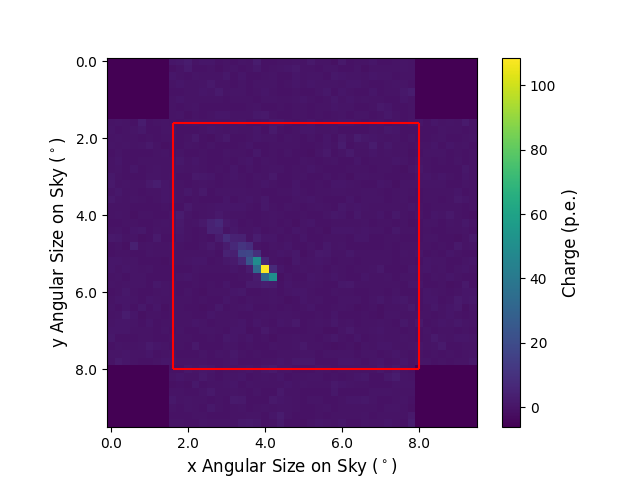
\includegraphics[width=0.7\textwidth]{figures/gammacut.png}
  \caption{A charge image from a simulated $\gamma$-ray event from the point source run dataset as described in section \ref{Datasets}. The region that survives the geometry cut is highlighted in red, the holes in the camera geometry to accommodate the flasher calibration system can be seen in the corners.}
  \label{fig:gammacut}
\end{figure}

\begin{figure}
  \centering
  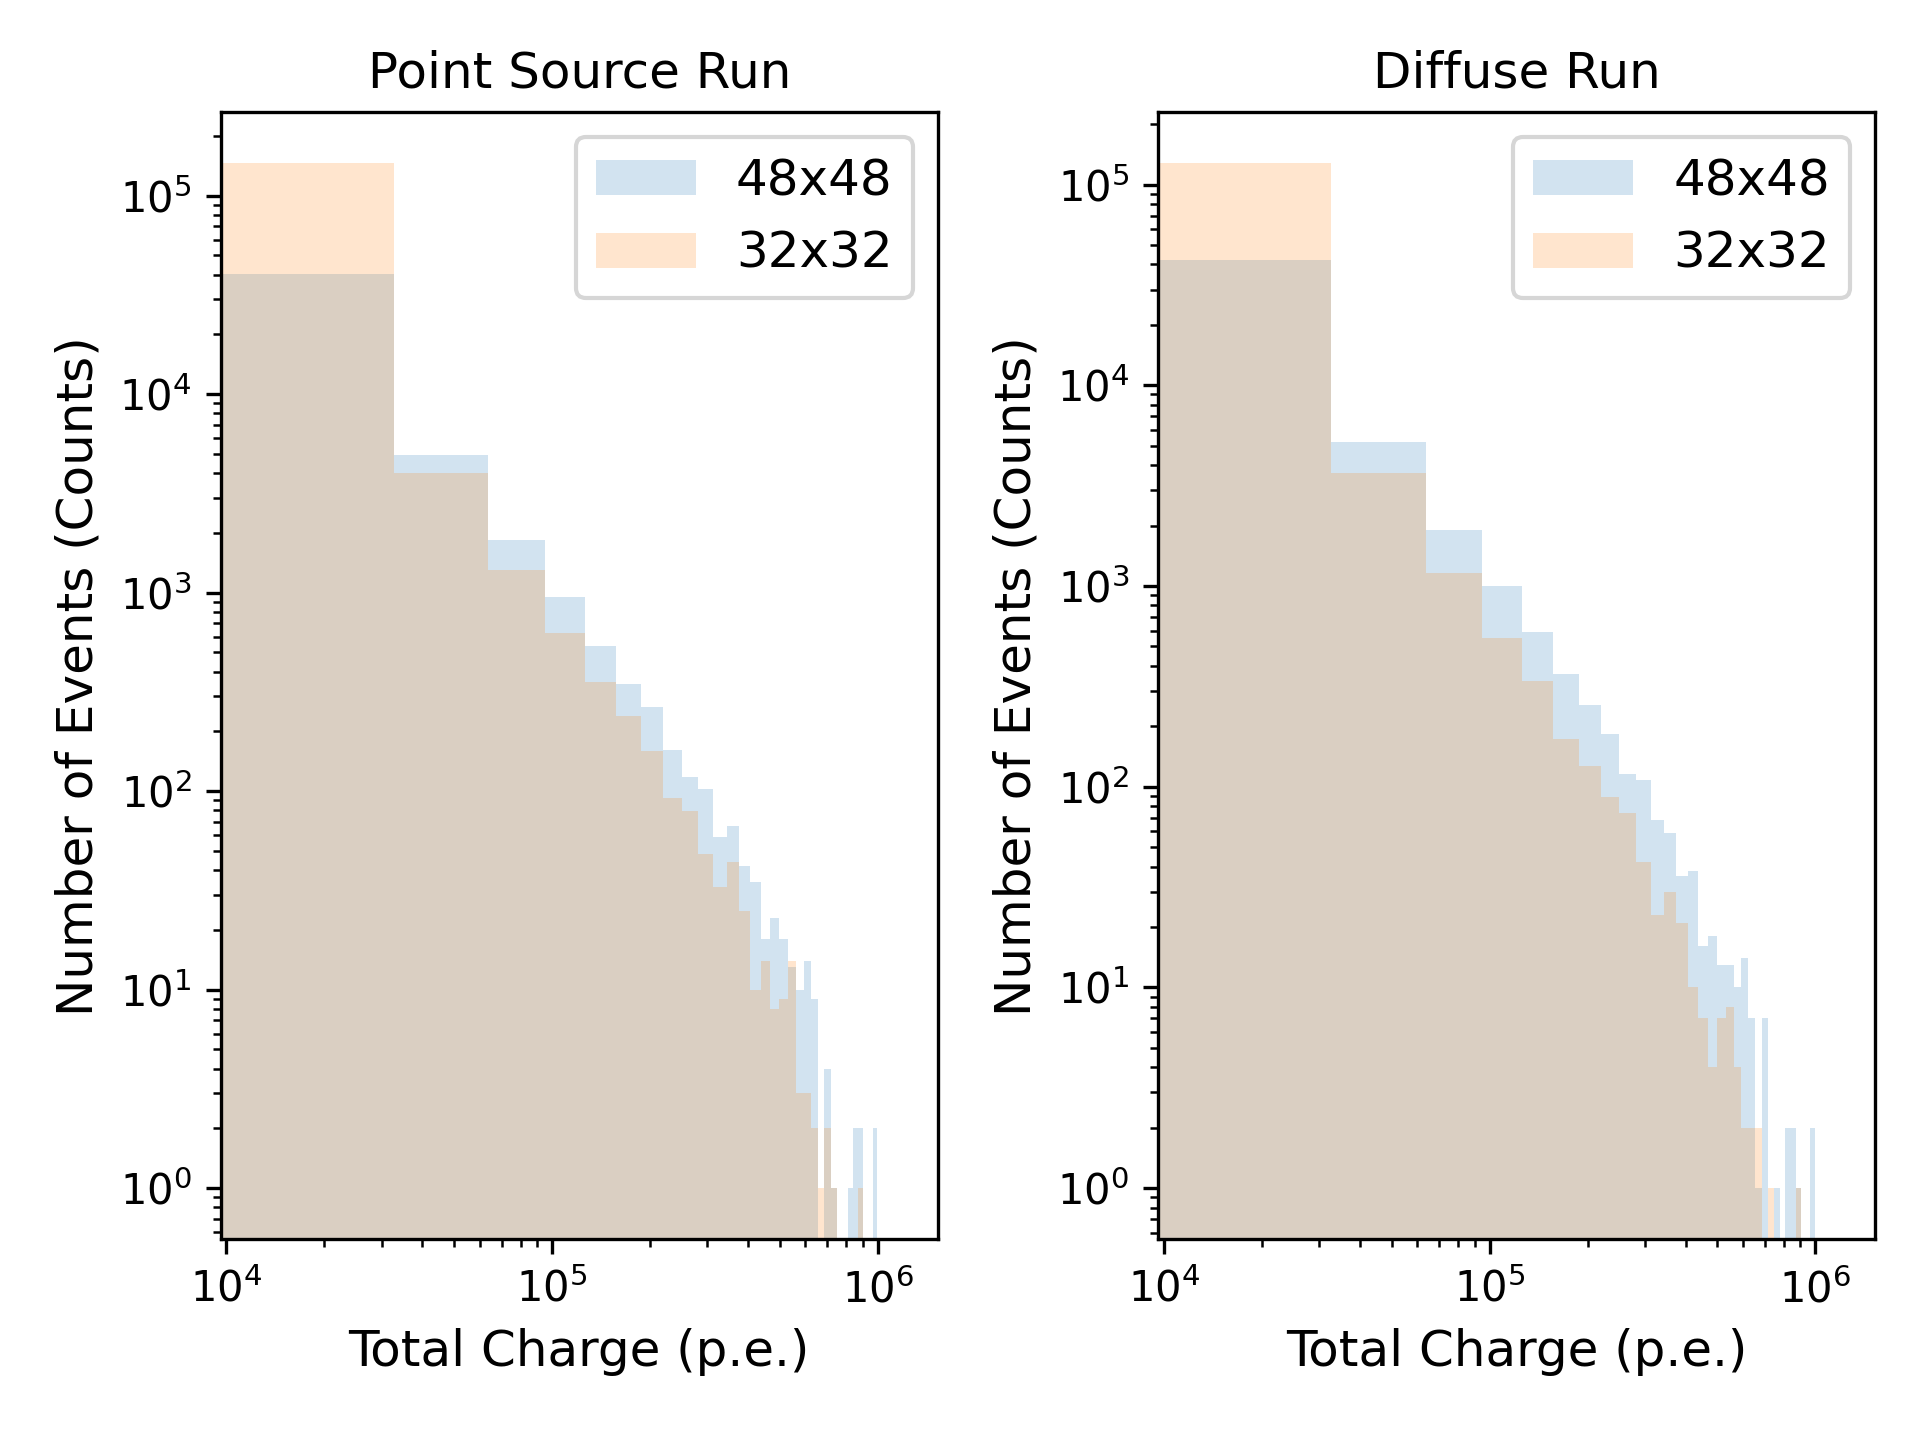
\includegraphics[width=0.7
  \textwidth]{figures/chargehistlog.png}
  \caption{Total integrated charge from all four telescopes over the two datasets used, as described in section \ref{Datasets}. Comparisons between the complete camera (48x48) and the cropped central region (32x32) are shown.  Most of the charge losses appear to be Night Sky Background photons as the two distributions are smooth and close together. The same logarithmic binning is used for both the cropped and uncropped regions.}
  \label{fig:chargehist}
\end{figure}
In order to perform our analysis, we used the \textit{Keras} (v.2.1.5) \cite{Keras} deep learning Python package with the \textit{Tensorflow\_gpu} (1.7.0) backend \cite{tensorflow}. We also used the \textit{scikit-learn} \cite{scikit} (v0.21.3) and \textit{matplotlib} (v.3.1.1) \cite{matplotlib} packages to analyse and plot the results. The analysis pipeline we developed to perform this is illustrated in Figure \ref{fig:wavelearn}. Similarly to \cite{Shilon}, we use a mixture of convolutional layers and recurrence (specifically ConvLSTM2D layers, algorithmic details of which can be found in \cite{shi}) to robustly handle data from multiple telescopes. We compared four different techniques (Methods A-D) for classifying events on a like for like basis with these networks. These are summarised in Table \ref{table:methods} and detailed in the next three paragraphs. 

\begin{table}[ht]
    \centering
    \resizebox{\textwidth}{!}{
    \begin{tabular}{c|c|c|c}
    \textbf{Method} &\textbf{Pixel Maps Used} & \textbf{Ordering} & \textbf{Parameters}\\
    \hline
    A& Timing& Median Peak Time & 293,673\\
    B& Charge, Timing, Mean Amplitude, Peak Amplitude & Median Peak Time & 301,233\\ &FWHM, RMS, RT, FT& \\
    C& Charge & Size Parameter & 293,673\\
    D& Charge & Median Peak Time & 293,673\\
    \end{tabular}
    }
    \caption{Summary of methods used. The ordering of input channels into the ConvLSTM2D networks is as presented in this table. The number of trainable parameters is also shown, highlighting the effect of using a different number of channels in method B.}
    \label{table:methods}
\end{table}
Part of the challenge in \cite{Shilon} was developing an unbiased method to handle Cherenkov camera images that are from a non-square (typically hexagonal) pixel grid \cite{Hexagdly}.  CHEC has largely square pixel geometry, bar for holes in its corners to accommodate the flasher calibration system. In our work, in order to be conservative and minimise the risk of potential geometric bias in which event classifications might be affected by proximity to these corners (which could be the case if they were instead filled by constant values), we simply crop images to the central region of the camera. This can be seen in Figure \ref{fig:gammacut}. This is unlikely to have a serious effect on the signal from the EAS as our simulation set-up (described in section \ref{Datasets}) produces images where the shower is close to the centre of the camera (as shown in Figure \ref{fig:chargehist}). For the same reason, we also neglect in our analysis to take account of small amounts of `dead space' between CHEC photomultiplier blocks. This also does not affect the fundamental conclusions of this work, as they are on a differential basis. More advanced tools are currently under development to cope with these issues \cite{dl1dh} \cite{thomas}.

In method A, we use the available waveform information to generate a 2D timing pixel map across the camera plane. We then select the pixels that have a large waveform amplitude, and set the other pixels in the pixel map to zero, in order to highlight the position of the shower in the image. The location of the peaks themselves is found using a wavelet convolution of width 8 and the \textit{scipy} (v1.4.1) \textit{signal.find\_peaks\_cwt} function \cite{scipy}\cite{findpeaks}. These four timing pixel maps (one for each telescope) are then fed into the network without anything else, in the order of increasing median photon arrival time.

In method B, we feed in the integrated charge image (without pixel selection) as the first channel to the ConvLSTM2D. We then feed in the timing pixel map created using the same technique as Method A as the second channel, and similarly cut 2D pixel maps of six other parameters from the smoothed waveform: the mean amplitude, the peak amplitude, the root mean square value (RMS), the full width at half maximum (FWHM, calculated using a B-spline interpolation \cite{scipy}), the pulse rise time (RT) and the pulse fall time (FT) relative to the peak of the waveform. Both the RT and FT are calculated using a change-in-gradient method. This results in four images each with eight channels being fed into the ConvLSTM2D; examples of these pixel maps are shown in Figure \ref{fig:wfplot}. These channels are treated as extra dimensions in the input tensor, in the same way that Red, Green and Blue channels would be for a colour image.

Method C uses only charge images, ordered such that those with the largest total charge appear first in the LSTM sequence (as in \cite{Shilon}). It should however be noted that we do not perform an exact replication of the method in \cite{Shilon}. This is due to a number of factors. Firstly, we consider different instruments with differing camera designs and operational energy ranges. Secondly, we use a marginally different ConvLSTM2D network architecture (due to the CRNN code from \cite{Shilon} being proprietary), this differs from the CRNN architecture in that recurrent (LSTM-like) features are included from input layer until the final layer of the network (though the basic principle of merging convolutional and recurrent features is the same). We also use differing hyperparameters, partially due to this different architecture, and partly because the differing plate scales and operational energy ranges of the H.E.S.S.-1 cameras and CHEC means that there is no guarantee that the ideal hyperparameter choice will be the same for both instruments. This hyperparameter choice can have a significant effect in CNN-based analysis \cite{hyperopt}. Finally, in order to test the efficacy of CNN-based background rejection against electrons, we include these (realistically) in the analysis whereas \cite{Shilon} did not. This would cause differences with the training of any machine learning classifier (particularly in the diffuse case) as there are two nearly identical data samples with differing class assignments.

\begin{figure}[ht]
  \centering
  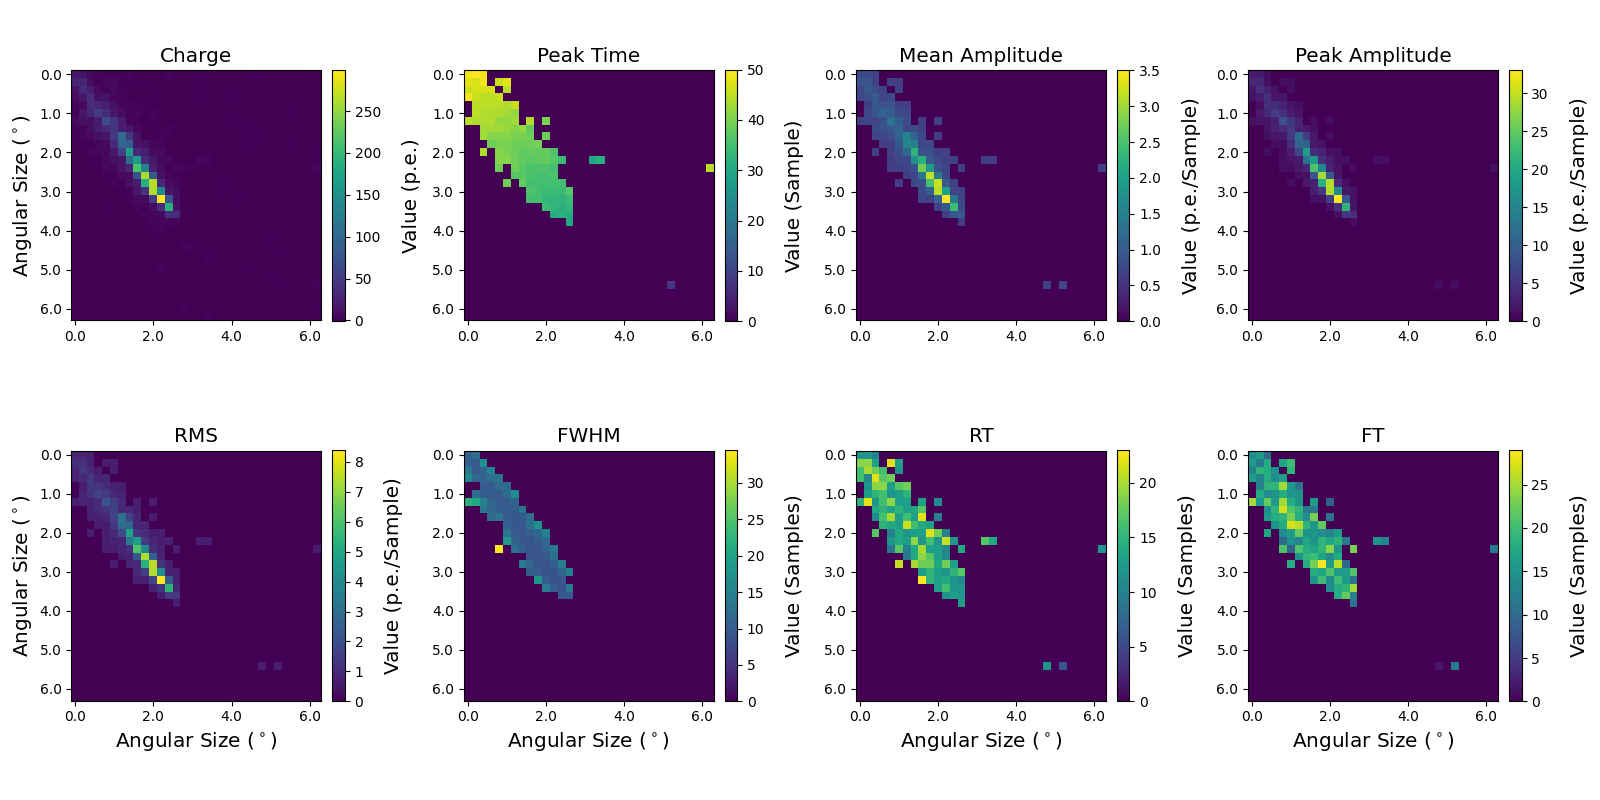
\includegraphics[width=\textwidth]{figures/56tgamma.png}
  \caption{As an illustration of the different pixel maps used with Method A, this figure shows pixel maps used (cut to the central region of the camera) from a 56 TeV $\gamma$-ray event in the point source dataset for one telescope. Note that these pixel maps are normalised prior to analysis, and that 1 sample represents approximately 1ns.}
  \label{fig:wfplot}
\end{figure}
In method D, we extract the median photon peak time from the waveforms and use this as a time proxy to order the images in place of the sum of the photomultiplier charges (as used in method C). In this case the only images actually fed to the network are those of integrated charge. As such the only difference between methods C and D is the order in which the charge images for an event are fed into the ConvLSTM2D, such that we can test what effect this has. Therefore methods A, C and D all result in 4 images each with 1 channel (i.e. grayscale) being fed into the ConvLSTM2D network.

The datasets used, along with all training hyperparameters (see Table \ref{table:hyperparams}), were the same across all the four methods during the initial training. As this is intended as a differential study, we did not perform hyperparameter optimisation. Whilst there are Bayesian methods such as hyperopt \cite{hyperopt} for performing hyperparameter optimisation with CNN-based classifiers, it would not be trivial to cross-optimise the networks fairly across the four methods described here and it would also involve currently unfeasible computational cost given the size of our datasets. Optimising the networks for say method B might disadvantage Method A unfairly. As such, we believe the least biased option is to use default hyperparameter options across the four methods. The ConvLSTM2D network architecture was also identical across the four methods, with the exception of the number of channels in the input vector (1-8).  This architecture is shown in Figure \ref{fig:model}.

\begin{table}[ht]
    \centering
    \resizebox{0.7\textwidth}{!}{
    \begin{tabular}{c|c}
    \textbf{Hyperparameter} & \textbf{Value}\\
    \hline
    Batch Size & 50 \\
    Training Epochs & 30 \\
    Training Optimiser & Adadelta \cite{adadelta} \\
    Adadelta Learning Rate & 1.0\\
    Adadelta Decay Factor &0.95 \\
    Output Layer Activation Function & Softmax\\
    \end{tabular}  
    }
    \caption{Training hyperparameters used; these were the same throughout all the networks during the initial training for both the point source and diffuse cases. The diffuse ES runs also used these hyperparameters.}
    \label{table:hyperparams}
\end{table}

\begin{figure}
  \centering
  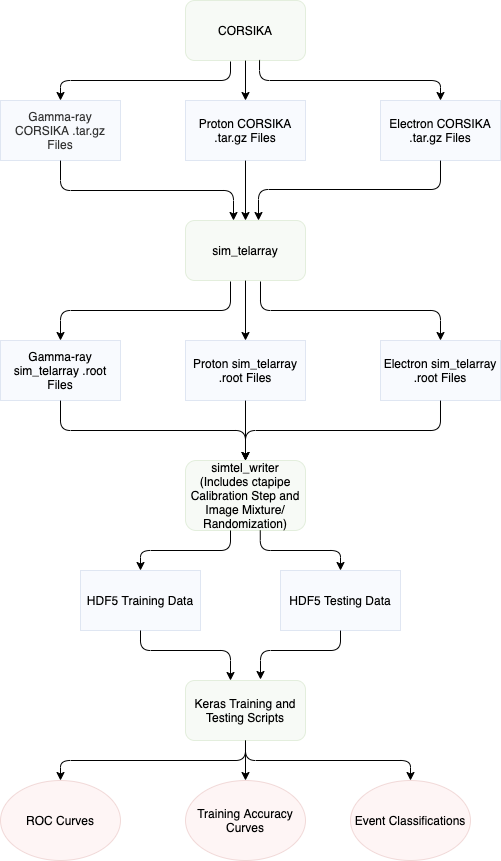
\includegraphics[width=0.7
  \textwidth]{figures/waveformstructure.png}
  \caption{The analysis pipeline used to generate the results in this paper. Ellipses denote analysis products, cornered rectangles denote stored files and rounded rectangles denote code elements.
  }
  \label{fig:wavelearn}
\end{figure}

\begin{figure}
  \centering
  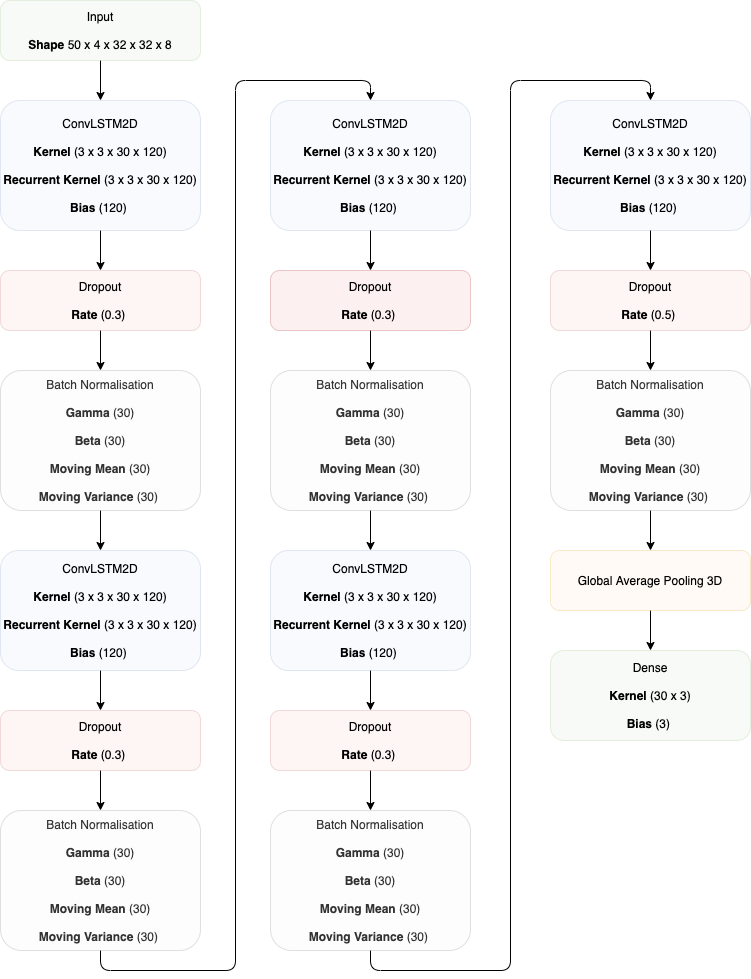
\includegraphics[width=0.9\textwidth]{figures/Newfig3.png}
  \caption{Example of our CNN-based ConvLSTM2D architecture. The only difference between the various methods A-D was the shape of the input vector, as some methods used more pixel maps than others.
  }
  \label{fig:model}
\end{figure}
In order to prevent over-fitting, the ConvLSTM2D layers are followed by dropout and batch normalisation layers, and recurrent L2 regularisation \cite{Keras} is employed on the first two ConvLSTM2D layers. At the end of the network, global average pooling is used to connect to a final dense output layer of size 3 with a softmax activation function. The network is trained for 30 epochs with a batch size of 50 events per step, where the images and pixel maps have amplitudes normalised to the range [0,1]. There is a question over the efficacy of normalisation of IACT images with CNN-based methods as it can potentially prevent generalization, but in this case we observed superior overall training performance when the images were normalised.

\section{Results} \label{Results}
\subsection{Initial Results}
 The initial training took approximately 3 days on a NVidia 1080Ti GPU for each ConvLSTM2D network, meaning the training time for the results presented in Figures \ref{fig:trainlog}, \ref{fig:ROC} and \ref{fig:ROC2} was around a month. Each network for each method (A through D) and each of the two datasets (point source and diffuse) was trained from scratch independently, so each sub-figure in Figure \ref{fig:ROC} represents the test results for a uniquely trained classifier (the results from which are re\-plotted in Figure \ref{fig:ROC2}). We do not mix classifiers trained on different datasets, so classifiers trained on point source data are tested on (previously unseen) point source data, and not diffuse data. As such, and given the fact that there is no preferential direction in any of diffuse data CORSIKA/sim\_telarray events (as seen in Table \ref{table:Datasetparams}), the diffuse data results demonstrate classification power based solely upon shower morphology. Training accuracies as a function of epoch for this initial training are shown in Figure \ref{fig:trainlog}. This training was a significant computational task, and represents the limit of what can be performed with a single GPU. It should also be noted that in this particular use case, the `Compute Capacity' (NVidia's measure of a GPU's specifications) of the GPU is an important attribute due to the presence of RNN features in our network. Additionally, having a large amount of VRAM allowed for the processing of large datasets.
 
 \begin{figure}[t]
  \centering
  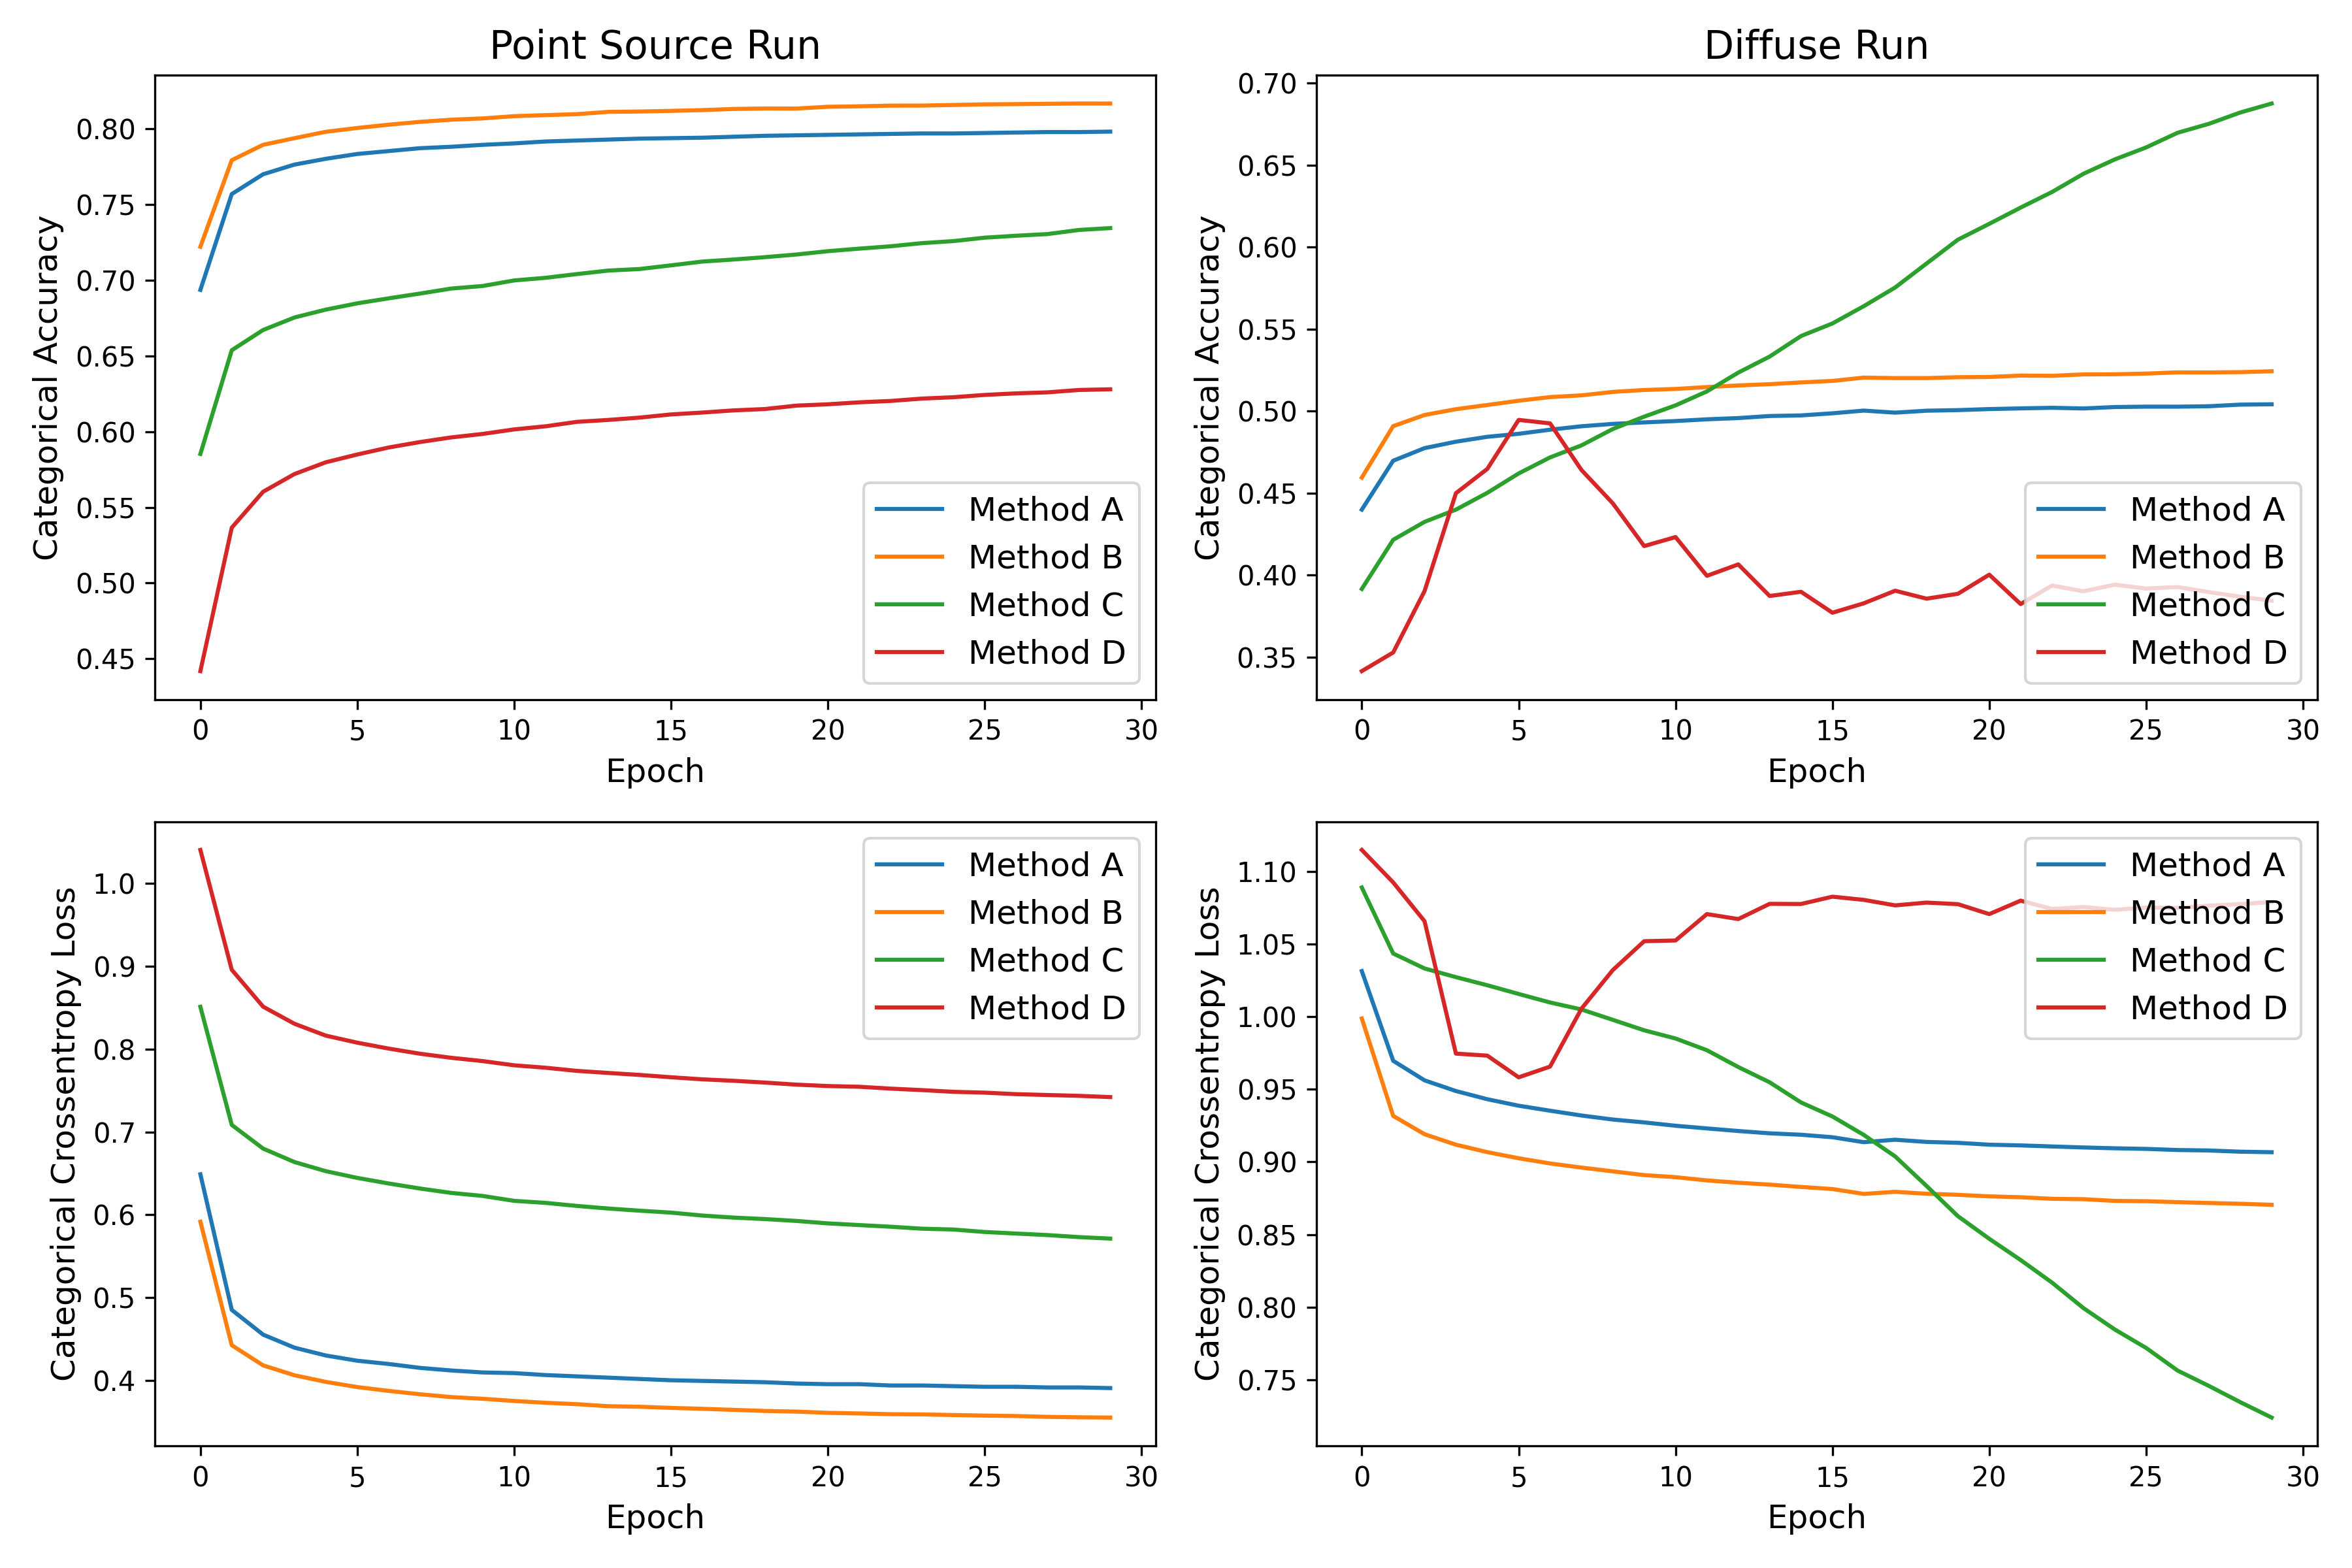
\includegraphics[width=\textwidth]{figures/trainlog.png}
  \caption{Initial training losses and accuracies for the four methods computed using the training dataset. Reasonable convergence is achieved for most methods given finite computational resources, but methods C and D in the diffuse case show some evidence of overtraining given their poor performance on the test data. This overtraining is evident here by either inversion or runaway acceleration in the loss function. It should also be noted that categorical accuracy and AUC values are not identically calculated metrics and the absolute values can differ.
  }
  \label{fig:trainlog}
\end{figure}
\begin{figure}
  \centering
  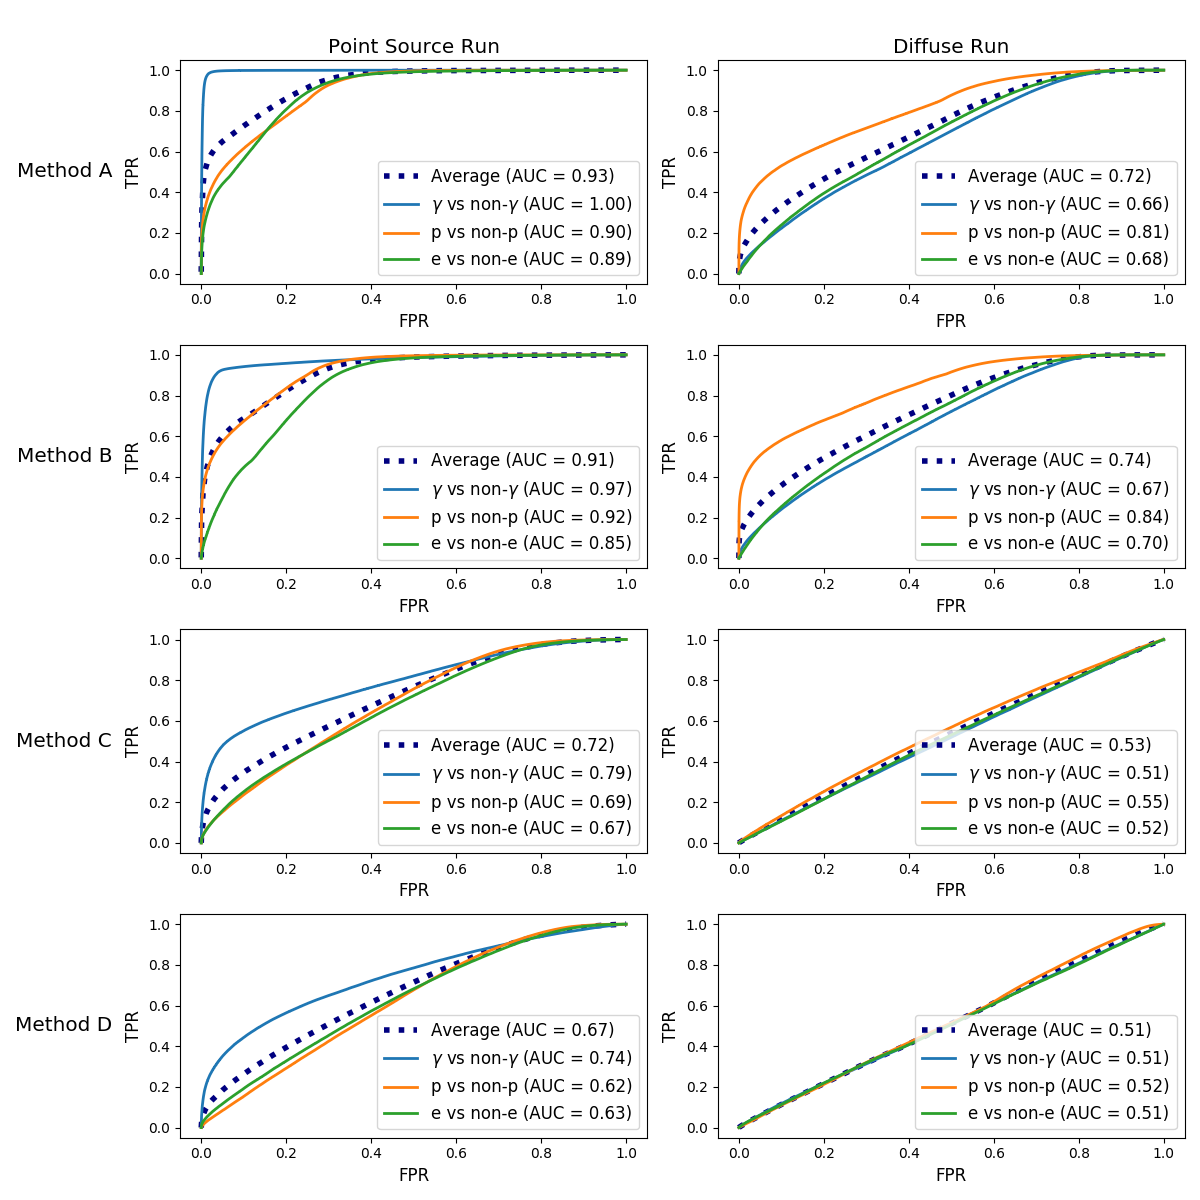
\includegraphics[width=\textwidth]{figures/final_newlabels.png}
  \caption{Receiver Operator Characteristic (ROC) curves for the four methods described showing the True Positive Rate (TPR) against the False Positive Rate (FPR). The Area Under Curve (AUC) performance metrics (the integral under these curves) are also shown. Deep learning analyses typically consider one versus all scenarios when calculating ROC curves \cite{scikit}, which is what we display here.  This means we consider if an event is classified a $\gamma$-ray or not a $\gamma$-ray when calculating the FPR and TPR in the multi-class scenario. Macro-averages across the three classes are also shown. It should be noted that the AUC results here and in Figure \ref{fig:ROC2} are only quoted to 2 decimal places and there are $\sim$700,000 testing events. As such, even in the optimal point source case, there are a number of misclassified events (i.e. $\sim$5500 $\gamma$-hadron misclassifications and $\sim$7000 $\gamma$-electron misclassifications for method A).
  }
  \label{fig:ROC}
\end{figure}
\begin{figure}
  \centering
  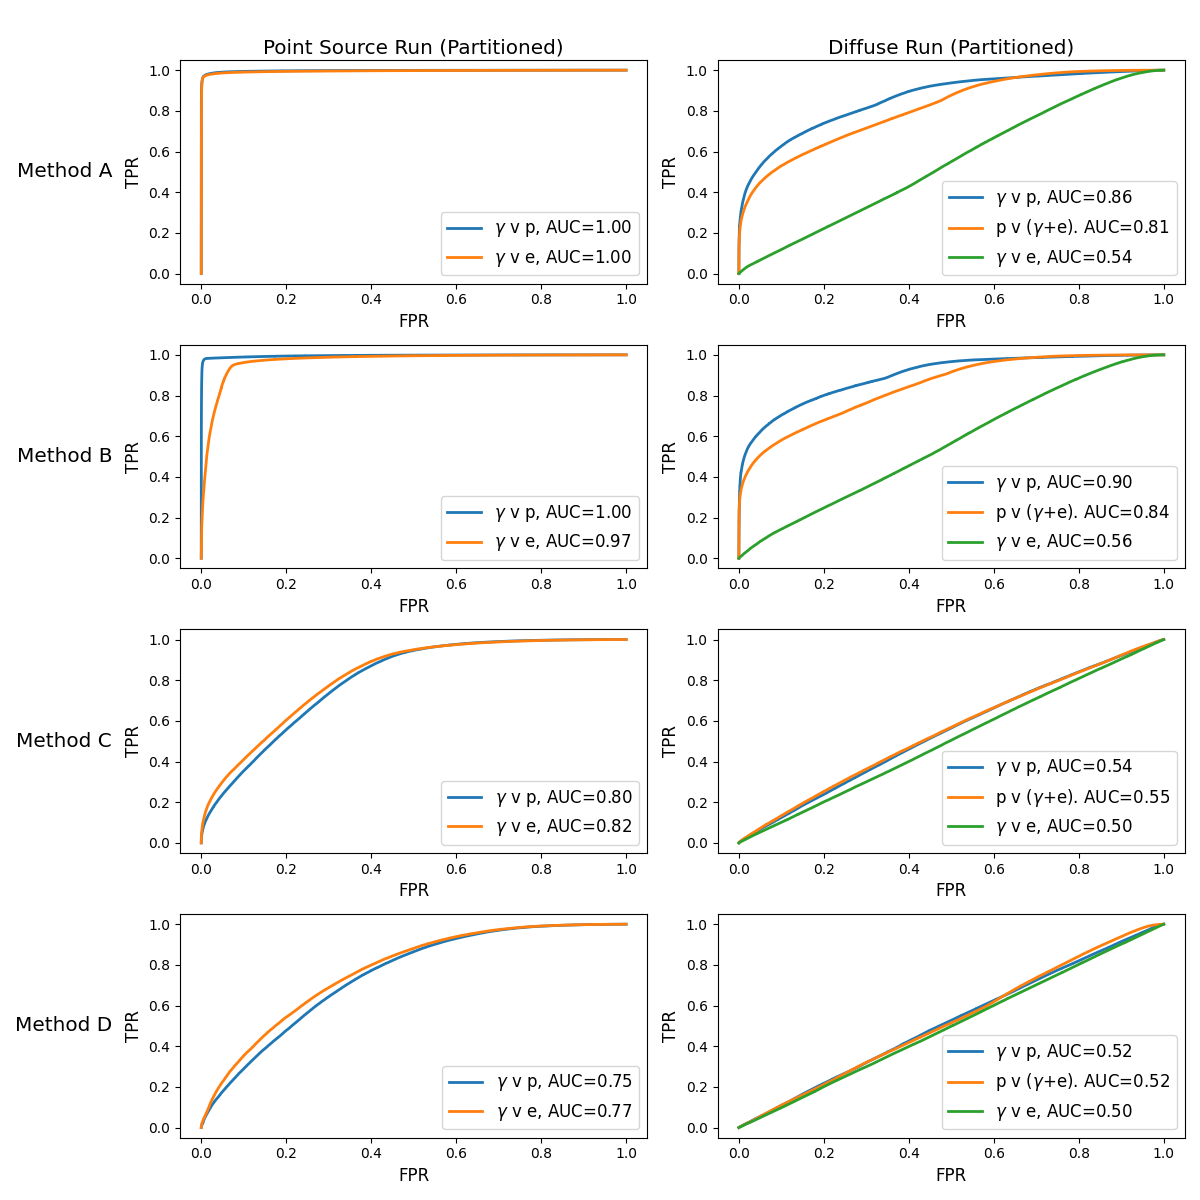
\includegraphics[width=\textwidth]{figures/abelardo.png}
  \caption{The same results from Figure \ref{fig:ROC}, this time shown in an astrophysical context. In this case we remove the other particle classifications from the analysis and consider only test FPR/TPR between various particles. In the point source run case, we consider the ROC curves for classification between $\gamma$-rays and protons and between $\gamma$-rays and electrons. This demonstrates the combined classification power of both morphological and directional information. The equivalent curves for the diffuse case highlight solely the morphological classification power. The proton versus ($\gamma$+e) curve demonstrates the difficulty  of distinguishing between $\gamma$-rays and electrons.
  }
  \label{fig:ROC2}
\end{figure}

\begin{table}[t]
    \centering
    \resizebox{\textwidth}{!}{
    \begin{tabular}{c|c|c}
    \textbf{Method} & \textbf{Point Source Run Classification Rate (Hz)}& \textbf{Diffuse Run Classification Rate (Hz)}\\
    \hline
    A & 308 & 296\\
    B & 240 & 231\\
    C & 339 & 320\\
    D & 308 & 336\\

    \end{tabular}  
    }
    \caption{Classification rates (the number of classifications per second) based on testing against $\sim$100,000 events for each method using 4 telescopes. Note that due to the LSTM features in our network this is substantially slower than classifications can be performed for Mono-telescope analysis ($\sim$1 kHz). This is also dependent on the GPU used (a NVidia 1080Ti in this case), and the data loader has not been fully optimised for speed. The test system had 32GB of Random Access Memory and operated at a clock speed of 1866 MHz.}
    \label{table:speed}
\end{table}
 \begin{figure}[t]
  \centering
  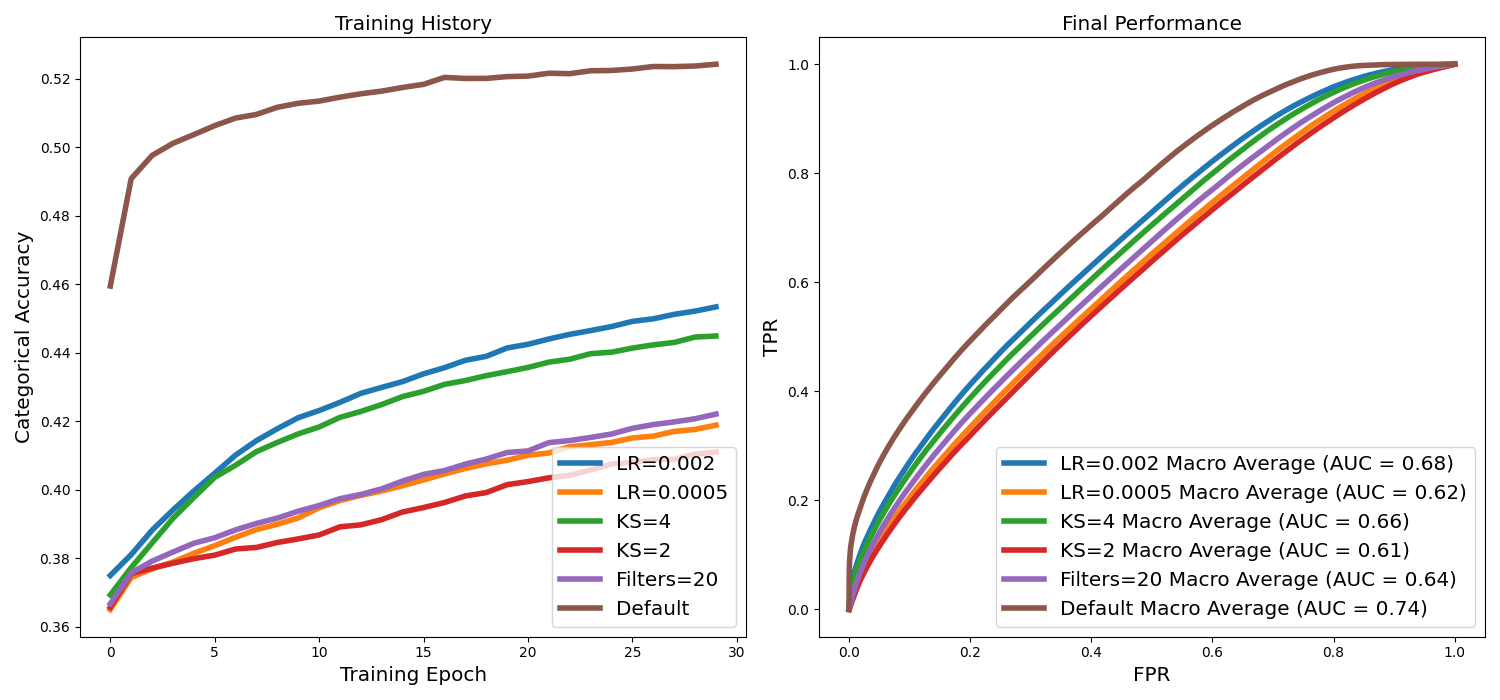
\includegraphics[width=\textwidth]{figures/modhyp.png}
  \caption{This plot shows the effect of modifying the hyperparameters for training Method B on the diffuse data. Left: The categorical accuracy as a function of epoch for the modified hyperparameter training runs. Right: The associated test ROC curves.
  }
  \label{fig:modhyp}
\end{figure}
\subsection{Difficulty in Identifying Classification Features}
Determining the source of classification power with CNN-type classifiers is non-trivial. Whilst gradient and perturbation based attribution techniques have been developed for standard single-image CNN classifiers (which can produce heat maps showing pixels relevant for classification) \cite{deepexplain}, open source packages for this do not currently extend support for such methods to the multiple image ConvLSTM2D case. As such, we are forced to interpret performance of these classifiers on different datasets in order to infer the information being used for classification. In our case, the results for the point source run and methods A and B achieve high performance metrics, but it appears as if this is as the classifier is largely using the directional information about the shower to perform classification, as opposed to using morphological features in the images. This can be seen in Figures \ref{fig:ROC} and \ref{fig:ROC2}, as the classifier differentiates between $\gamma$-rays and other classes easily in the point source case for methods A and B, but not between the diffuse protons and electrons. However, it is noteworthy that the ConvLSTM2D network performs this task so well and that methods A and B perform this in a superior way to methods C and D. This bodes well for future studies into directional reconstruction using CNN-based methods, as well as demonstrating the merit for multi-task deep learning studies that attempt to perform the tasks of event classification and directional reconstruction simultaneously (such as \cite{jacquemont}). This knowledge of the strong directional sensitivity of CNN-type methods can be used to inform the design of future CNN-based analysis pipelines for CTA.

In the diffuse case (where all three event classes come from an even spread of directions), methods C and D overtrain and cannot distinguish between any of the event classes. However the timing based methods A and B appear able to perform good event classification based on shower morphology in Figure \ref{fig:ROC2} between the (combined) $\gamma$-ray and electron showers versus protons (that could be optimised further), however they cannot distinguish between the $\gamma$-ray and electron induced showers. The classification rates for the four different methods are shown in Table \ref{table:speed}, despite using many more pixel maps method B classifies at $\sim 70\%$ the rate of the other methods. However, although including much more information than method A, method B doesn't appear to offer any significant improvement. This is likely as the timing information is likely to be the key component in the classification, though the marginally increased number of trainable parameters (as seen in Table \ref{table:methods}) for method B might disadvantage it slightly on a differential test basis.

\subsection{Effect of Hyperparameters}
In order to test the effect of varying hyperparameters, we ran additional training runs for Method B on the diffuse data. These runs were identical to the previous training runs for method B bar a single change each from the `default' hyperparameters shown in Table \ref{table:hyperparams} and Figure \ref{fig:model}. One run each had doubled and halved the Learning Rate (LR) from the default Adadelta value of 0.001, one run had all ConvLSTM2D kernel filter sizes (KS) set to 2x2, one with all filter sizes set to 4x4 and a final run with the number of filters per layer set to 20 rather than 30 (this value could not be increased due to VRAM constraints). The training accuracy curves (all showing reasonable convergence) and test results from this are shown in Figure \ref{fig:modhyp}. The `default' hyperparameter setup outperforms the alternatives, however this is to be expected as changing the \textit{Adadelta} optimiser parameters is not recommended by the developers of \textit{Keras} \cite{Keras}, and the 3x3 filter size option also provided the good results in the original ConvLSTM2D paper \cite{shi}. Whilst this gives us some idea of the spread in performance due to hyperparameter selection, this is not a substitute for an exhaustive hyperparameter space search, the optimal combinations of which are often not human-interpretable. The uncertainty associated with individual event classifications is also not trivial to obtain with CNN-type methods \cite{mike}\cite{gal2015}, and this is likely to be a necessary area of further development for these analysis techniques.

 \begin{figure}[t]
  \centering
  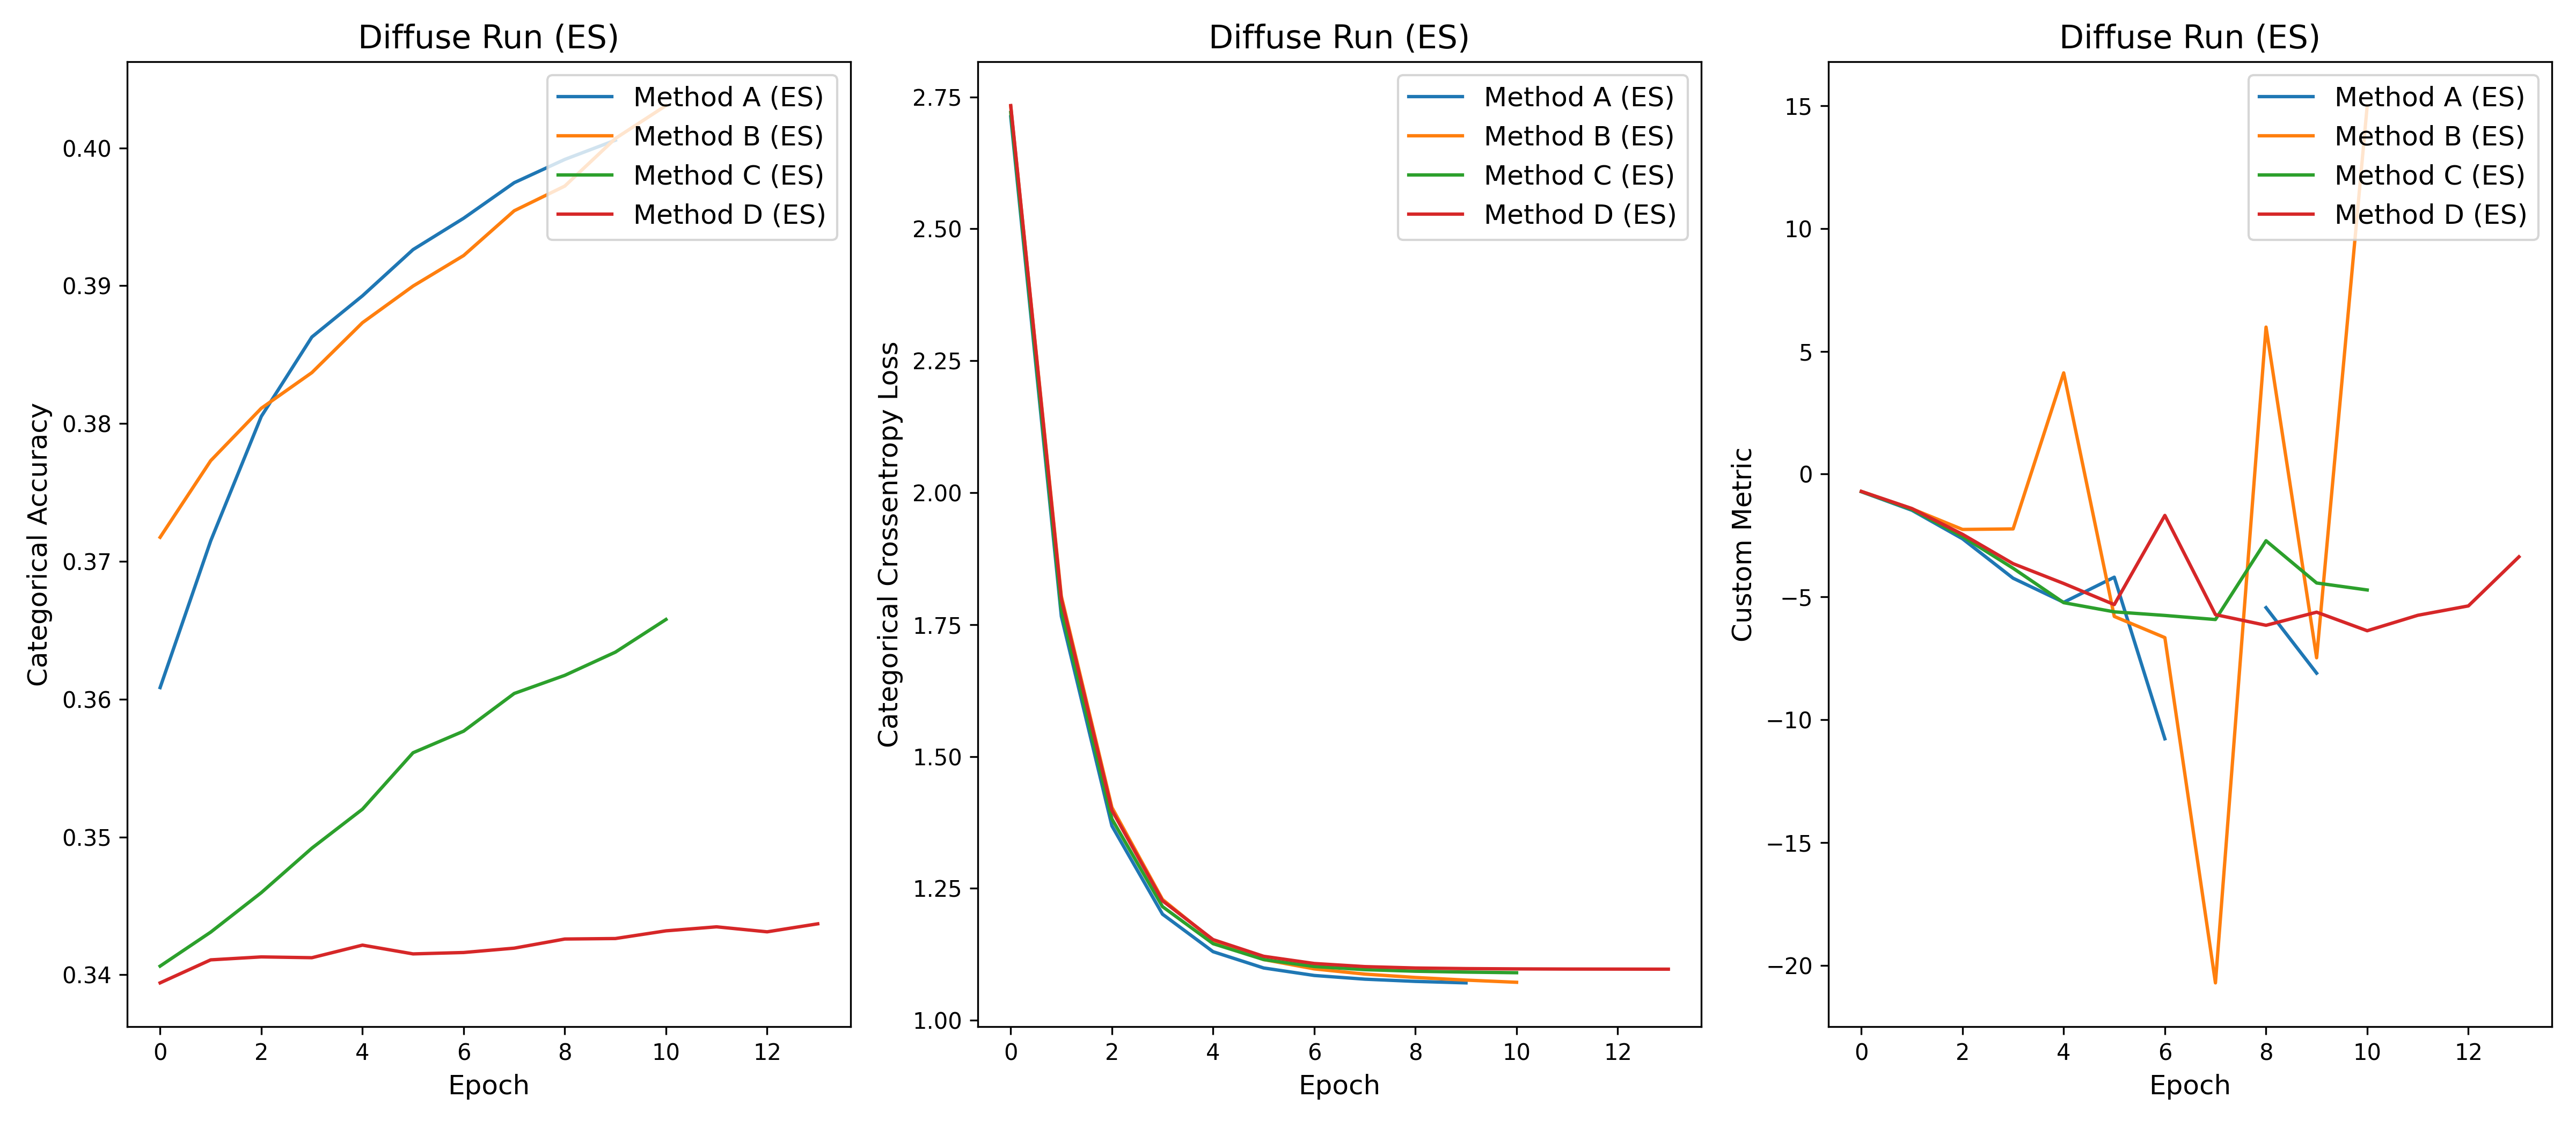
\includegraphics[width=\textwidth]{figures/trainlogES.png}
  \caption{Training total loss, categorical accuracy, and custom metric (M) values for the four ES runs, all on the diffuse data. The custom metric curve for method A diverges towards an infinite value due to finite numerical precision on epoch 7.
  }
  \label{fig:trainlogES}
\end{figure}

\subsection{Convergence and the effect of Early Stopping}
\begin{figure}
  \centering
  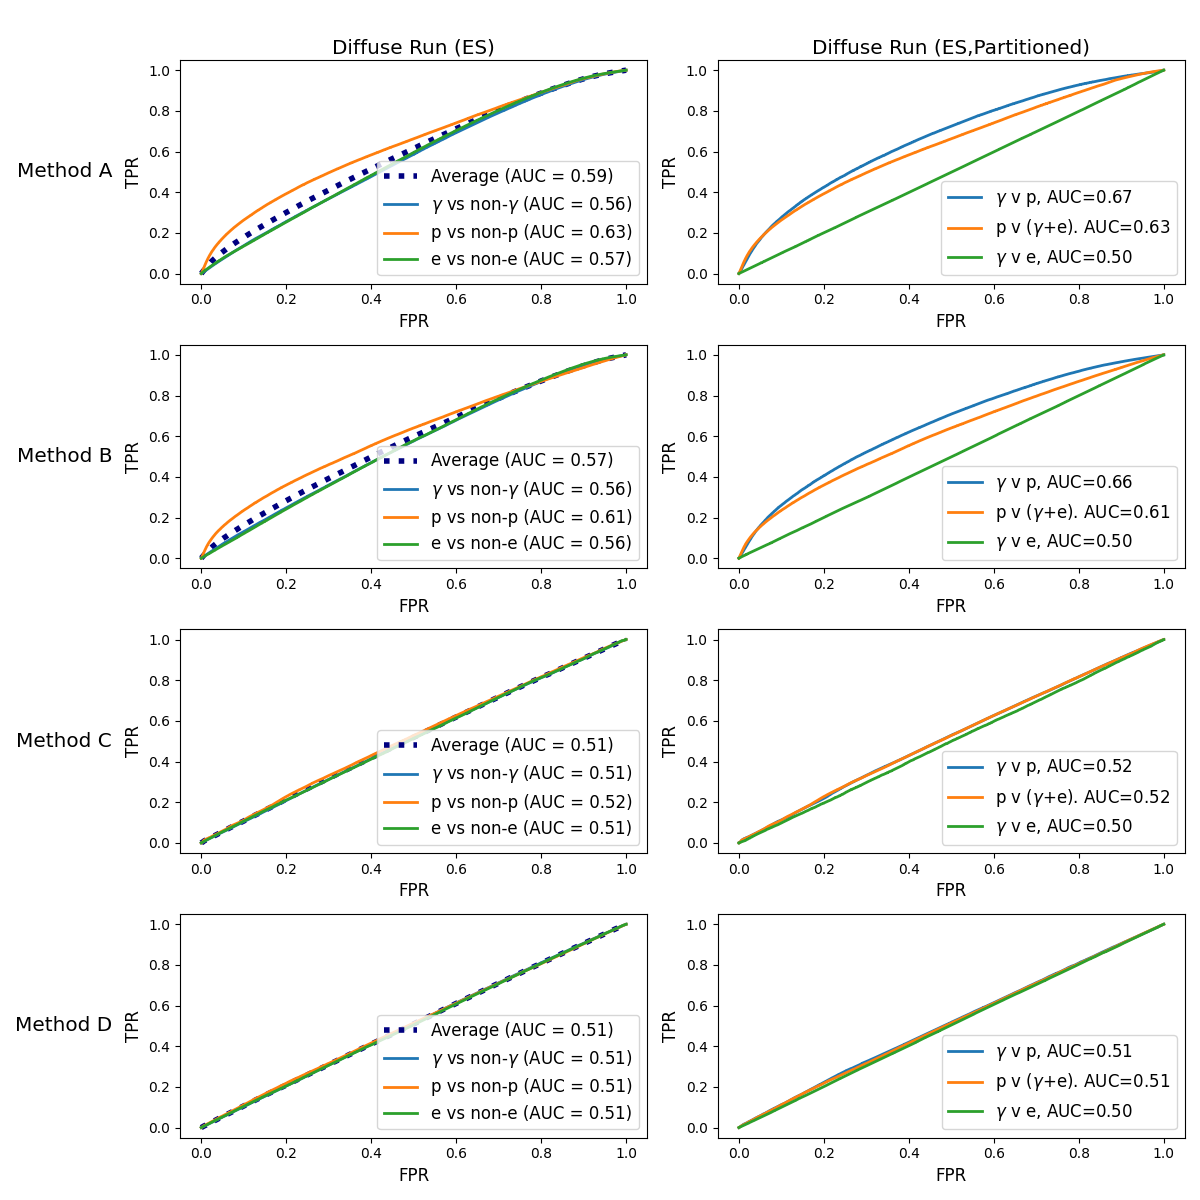
\includegraphics[width=\textwidth]{figures/esplot.png}
  \caption{This figure shows the final results from the ES runs, which are only trained and tested on diffuse data. Left: The results presented in the standard machine learning one versus all approach as in Figure \ref{fig:ROC}. Right: The same ES results shown in the astrophysical context of Figure \ref{fig:ROC2}.
  }
  \label{fig:ROC3}
\end{figure}

In order to investigate the influence of overtraining of methods C and D in the initial diffuse runs (as seen in Figure \ref{fig:trainlog}) with the original hyperparameter configuration from Table \ref{table:hyperparams} and Figure \ref{fig:model}, we ran additional training and testing runs on this diffuse data using this `default' configuration along with two early stopping criteria (that we reference by the abbreviation ES). Early stopping in \textit{Keras} allows for the stopping of training when there is an inversion in a chosen metric function, and for the restoration of the earlier optimal model weights obtained during training. In the case of preventing the overtraining scenario we observed for method D (where there's a clear inversion in the loss at epoch 6), the choice of this early stopping metric is the total loss function used during training. However, choosing such a metric to prevent the overtraining scenario we observed for Method C whereby there is undesired, runaway acceleration in the training data loss is more complex. As such, we implemented a custom second metric (M) of the form
\begin{equation}
    M=\frac{1}{0.7-0.8*L}
\end{equation}
where L is the total loss shown in for example \ref{fig:trainlog}. This L includes both the categorical cross-entropy loss and the regularization penalties which we explicitly sum over the first two ConvLSTM2D layers. We intentionally designed this metric as it has a turning point (that will trigger the \textit{Keras} early stopping) around the epoch that method C appeared to start overtraining in the original training runs. For both metrics we choose a \textit{patience} parameter of 3, representing the number of epochs to tolerate the inversion of the metrics.

The training curves and results from these ES runs can be seen in Figures \ref{fig:trainlogES} and \ref{fig:ROC3}. During the ES training for Method A, the early stopping was triggered on epoch 10, for Method B and C on epoch 11, and Method D on epoch 14. We still observe superior performance (and some ability to perform gamma/hadron separation using morphological information) for the timing based methods A and B, despite this early stopping procedure (which was human-engineered for Method C). As such, we believe the superior performance of methods A and B in the diffuse case cannot be solely attributed to a bias from the non-convergence of the initial training for methods C and D, and is a result of the charge-only dataset used for methods C and D rather than an effect due to the design or optimisation of the classifier network.

The charge-only methods \cite{Shilon} (methods C and D) perform poorly in our analysis in both the point source and diffuse cases (regardless of whether early stopping is used or not); this isn't to say that such charge-only methods could not function well given additional hyperparameter optimisation and image cleaning. We explained our motivation for not performing such hyperparameter optimisation in section \ref{Methods}. We seek simply to demonstrate the effectiveness of our timing techniques on a differential basis, which is confirmed by our results. As such, the absolute ROC, AUC, loss and accuracy values here should not be considered to be optimal for any of the four methods. It should also be noted that the realistic presence of electron events in the training datasets likely makes training the networks in the diffuse case significantly harder than straightforward $\gamma$-hadron separation given their similarity to $\gamma$-ray events, and this is likely part of the reason these two methods perform poorly in the diffuse case. Part of our reasoning behind these conclusions is that all four methods are affected to roughly the same extent ($\sim$0.2 AUC) by the change between (non-ES) diffuse and point source runs. Small variations in the accuracy values between the different methods could be statistical or due to hyperparameter configuration; averaging the results from multiple trials with different random seeds might help to confirm this, however this would be highly computationally intensive.

\section{Our investigation into identified features}
\begin{figure}[ht] 
        % read manual to see what [ht] means and for other possible options
        \centering 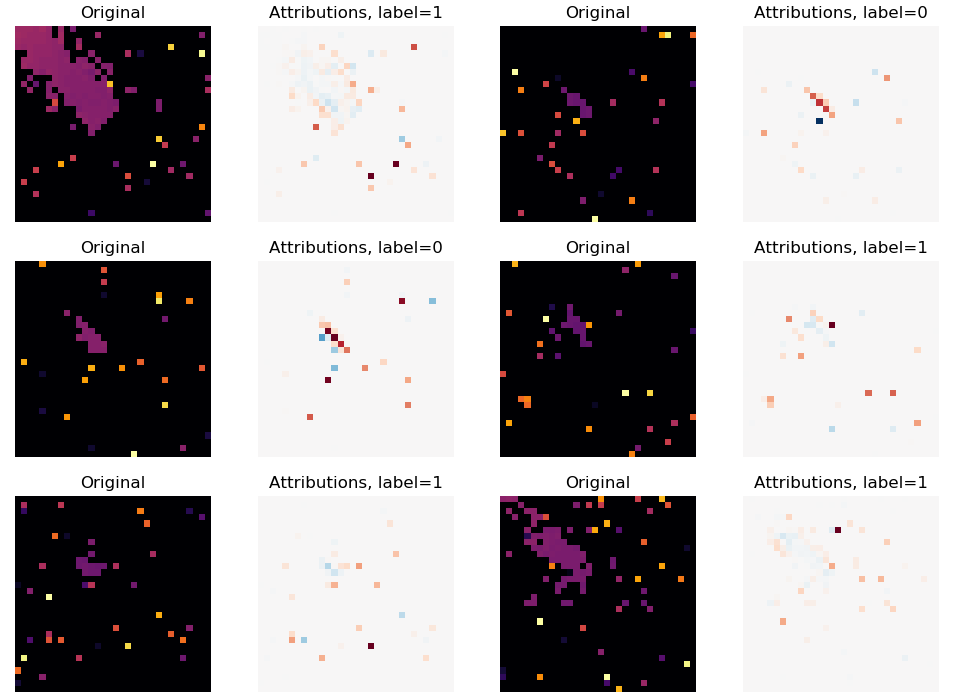
\includegraphics[width=1.0\columnwidth]{figures/lrp.png}

        % note that in above figure file name, "sr_setup",
        % the file extension is missing. LaTeX is smart enough to find
        % apropriate one (i.e. pdf, png, etc.)
        % You can add this extention yourself as it seen below
        % both notations are correct but above has more flexibility
        %\includegraphics[width=1.0\columnwidth]{sr_setup.pdf}
        \caption{
                \label{fig:lrp} % spaces are big no-no withing labels
                % things like fig: are optional in the label but it helps
                % to orient yourself when you have multiple figures,
                % equations and tables
                The results of our LRP investigations. Test images fed to the network are shown along with the feature maps associated with them, where deeper shades of red indicate the pixels that contributed the most to the classification as a gamma ray induced shower (labeled 0) or hadronic shower (labeled 1) and deeper shades of blue pixels that counted against the classification.  
        }
\end{figure}
CNNs and other machine learning techniques are frequently used as 'black boxes' across many disciplines. Given the many biases we have explored in earlier sections, this is a very bad idea. As such, we have undertaken to explore methods of identifying the features learned by our CNNs using CTA images. There are two established techniques for doing this, the first is to iteratively mask out features in input images and observe the change in CNN predictions. The second is to do a complicated weighted sum backwards through the network and identify the pixels that contributed most to a classification. We focus on the latter as it allows for pixels which counted against the classification to also be identified, specifically using the Layerwise Relevance Propagation (LRP) technique \cite{LRP}. This assigns a relevance to every $i$th neuron in layer $l$ in the network
\begin{equation}
r^{(l)}_i=\sum_j\frac{z_ji}{\sum_{i'}(z_{ji'}+b_j)+\epsilon\cdot\rm{sign}(\sum_{i'}(z_{ji'}+b_j)}r_j^{(l+1)}
\end{equation}
where $z_{ji}=w_{ji}^{(l+1,l)}x_i^{(l)}$, $w_{ji}$ is the weight associated with the $ji$th connection in the neuron, $x_i$ is an element of the input vector to a neuron, $b_j$ is a bias term and $\epsilon$ is a small term added to improve numerical stability. The ultimate values we want are the relevances for the input layer $r_i^{(1)}$.

Our results from applying this technique to a sample 2D convolutional network using the DeepExplain package are shown in Figure \ref{fig:lrp}. The images fed to the network in this case are the 2D timing histograms discussed in Section 4. It appears that the position of the shower in the image correlates well with the relevances calculated, and the correct features associated with hadronic interactions are being identified. The results do not change significantly for images of total integrated charge or by using alternative feature identification techniques. It is our belief that LRP will be a useful tool to compare the efficacy of neural networks trained with simulations against real data.

\section{Comparison to RFs}

Performing a fair comparison between existing BDT techniques and CNN-based methods is an involved problem, especially as CTA reference analyses have yet to be established. Whilst an initial comparison can be found in the Shilon et. al work \cite{Shilon}, currently unsolved questions about how to robustly perform such comparisons include the quantification of the computational cost, the management of the sensitivity versus robustness trade-off, and the correct way to co-optimise the classifiers. Whilst BDTs may be trivial to optimise, the same cannot be said for CNN-type methods, and this ultimately this might limit their practicability. This will be the subject of a future CTA consortium technical publication.

In this section we provide a crude comparison of our deep learning methods to Random Forest classifiers trained on the same data. Whilst a detailed comparison is difficult for these reasons, it is particularly important to demonstrate that attempting to train a parametric method on this extremely challenging dataset is not trivial. Additionally, a `Pythonic' tool for generating lookup tables suitable for generating the weight terms in the formula for mean reduced scaled width and lengths does not currently exist, so we simply use averaged length and width of the images (however in this special case of a very symmetric array looking at high azimuth it is unlikely to have a major effect).

To implement this, I reverse engineered the Hillas parameter extractor from ctapipe to extract Hillas parameters from the diffuse and point source training datasets used with the ConvLSTM2Ds. I then used the scikit-learn python package to train a conventional Random Forest conditioned on the existing training events, and tested them against the same test events. In order to test the effect of including electrons in the analysis, we also compare the accuracies of RFs trained and tested without these events (this was computationally prohibitive to investigate with the ConvLSTMs). The random forest classifier used the scikit-learn default hyperparameters, with 100 estimators and using the 'Gini impurity' to measure the quality of the split \cite{scikit}.

\begin{figure}[ht] 
        % read manual to see what [ht] means and for other possible options
        \centering 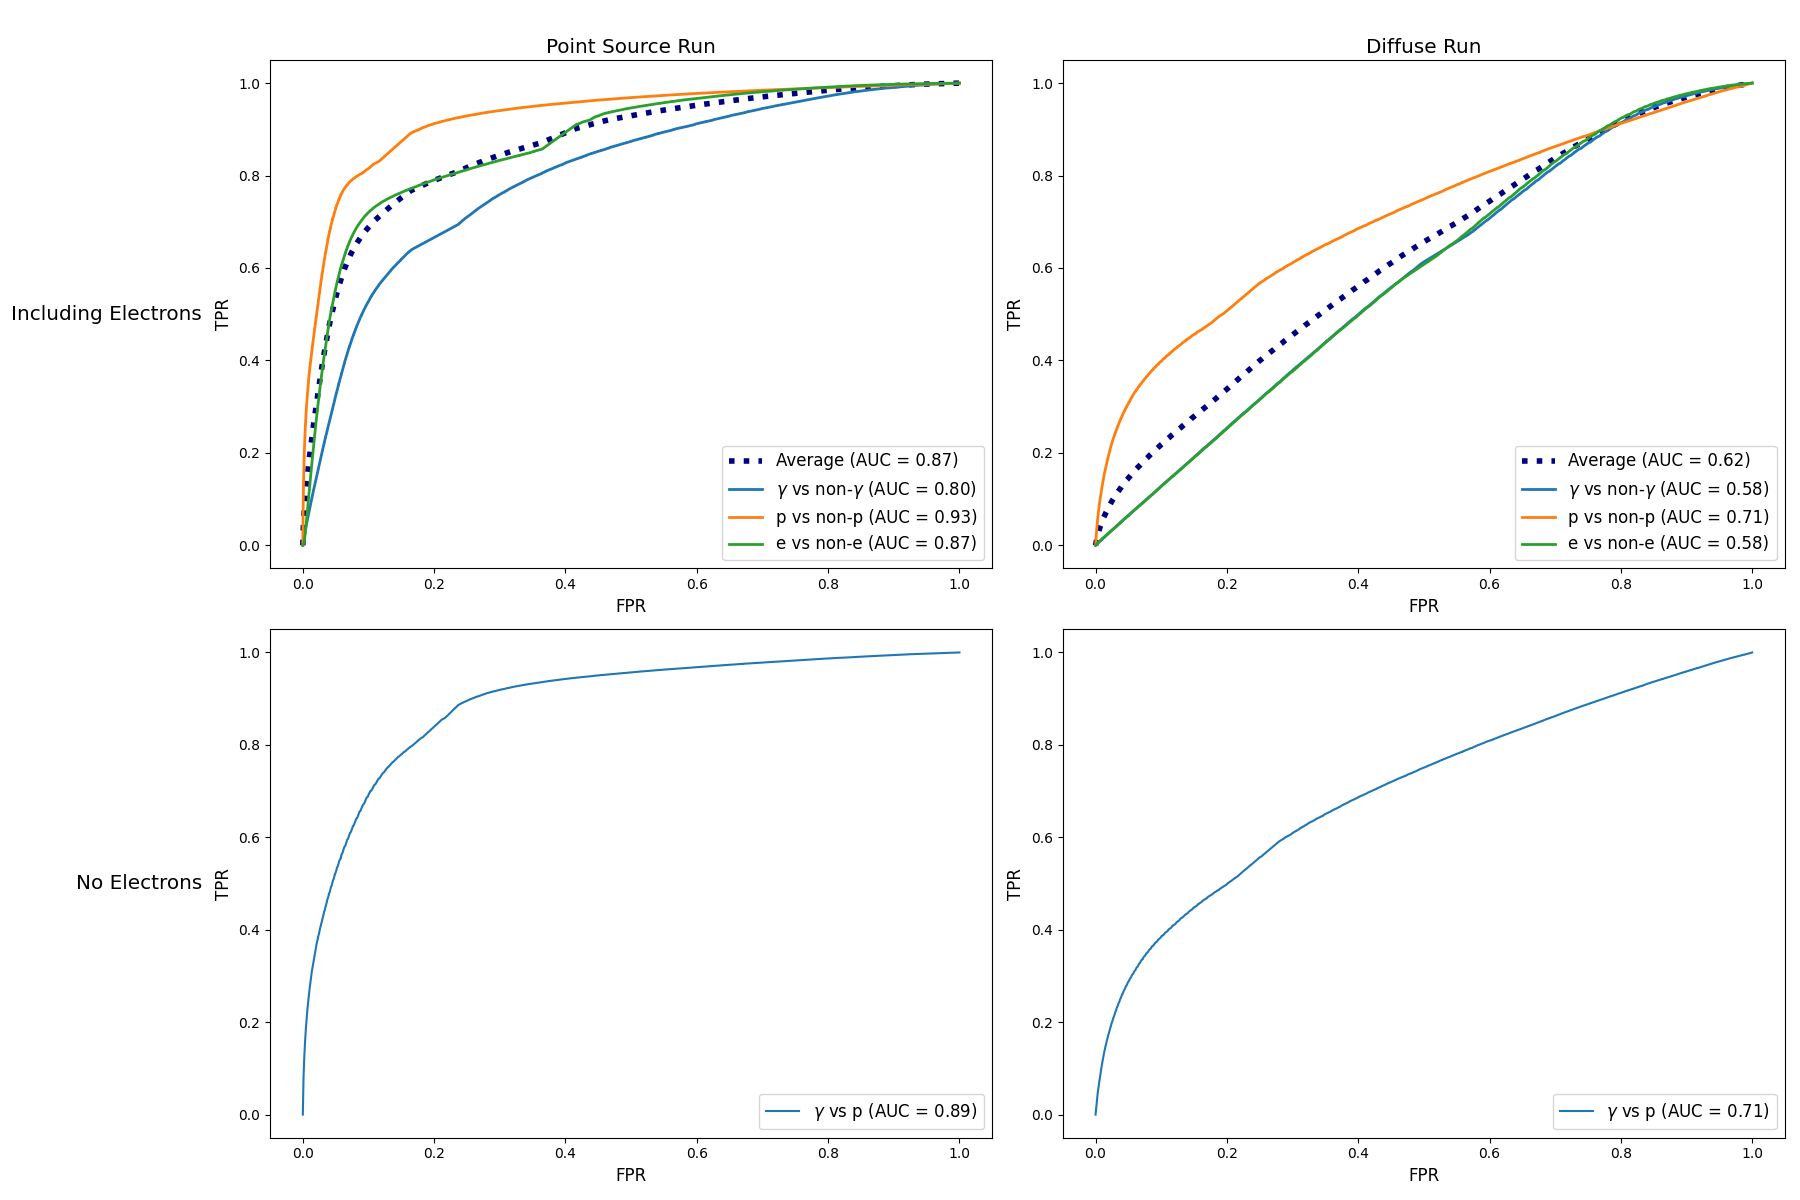
\includegraphics[width=1.0\columnwidth]{figures/rfplot.png}

        % note that in above figure file name, "sr_setup",
        % the file extension is missing. LaTeX is smart enough to find
        % apropriate one (i.e. pdf, png, etc.)
        % You can add this extention yourself as it seen below
        % both notations are correct but above has more flexibility
        %\includegraphics[width=1.0\columnwidth]{sr_setup.pdf}
        \caption{
                \label{fig:rfplot} % spaces are big no-no withing labels
                % things like fig: are optional in the label but it helps
                % to orient yourself when you have multiple figures,
                % equations and tables
                Point source and Diffuse RF test ROC curves with AUC values shown.
        }
\end{figure}

These clearly show (expected) inferior performances of the RFs on these data, as well as clearly demonstrating that the presence of electrons in the data has a significant effect on the average AUC value. However given the issues with applying CNN-type methods to real data explored in the next chapter, it is likely these RFs would still outperform the ConvLSTM on real data.

\section{Pseudosimulating Real Data Artefacts}

\section{Conclusions} \label{Conclusions}
We have investigated four methods of applying new deep learning methods to the task of classifying events for IACTs, finding that the use of timing information is an viable method of event discrimination against simulated hadronic air showers. Whilst not a full sensitivity analysis, we feel our results demonstrate the value in including timing information in future CTA deep learning analyses. This became possible thanks to the significant technical innovation that has gone into the design of CHEC and other similar modern Cherenkov cameras. However, we believe our work demonstrates that there is little prospect of CNN-based methods being used to filter out electron induced air showers, and so in future IACT deep learning studies (in the SST energy range) electrons should be treated as an irreducible background. That said, future IACT instruments may provide even more detailed images of EAS that might make electron event rejection feasible.

Another area of uncertainty related to this research is whether the representation of stereoscopic timing information in sim\_telarray is sufficiently accurate to be used for these purposes. In the absence of multiple SSTs existing on site this is difficult to currently test, however we speculate that it might be possible to overcome such errors by simply adding offsets to the timing histograms based on telescope pointing and shower direction.


\chapter{\label{ch:4-VERITASRealData} Challenges of Applying Deep Learning Event Classification Methods to Real Observations with VERITAS}
\minitoc
\begin{abstract}
    It is becoming increasingly recognised that artefacts in real IACT data have the potential to seriously disrupt the efficacy of deep-learning-based event classifiers. This issue has so far been relatively poorly understood, and these artefacts are not modelled in simulations. In this chapter, we attempt to investigate the difficulties in performing observations with real observations from VERITAS when a deep learning event classifier is used. In contrast with previous efforts with H.E.S.S. data, we do not use tailcut image cleaning with charge data. We also explore the limitations of using a custom simulation approach as a means of mitigating real observations issues, as well as the utilisation of Bayesian optimisation (which for the first time we attempt to use against real IACT data). After developing a pipeline for performing deep learning analysis with VERITAS data, we present the first detection of the Crab Nebula using a deep learning event classifier with a stereoscopic IACT array. We conclude that with current computational power and techniques, the complexity and cost of optimising deep learning event classifiers in this manner is significant. This limits the current applicability of these methods to current generation instruments or data from CTA.
\end{abstract}

\section{Introduction}

In this chapter, we explore potential issues with the application of CNN-based classifiers that have been trained with simulations against real low-level data from VERITAS. In contrast with Chapter \ref{ch:3-TimingInfo} we cannot use timing information with VERITAS. This is as the telescope optical path delays create a $\sim$ 7ns timing jitter in the peak time results. Therefore we concern ourselves with methods using integrated charge-only images, similar to more conventional IACT analysis. Given the results in Chapter \ref{ch:3-TimingInfo}, where we found that there was no potential for separating electron-induced events from $\gamma$-ray events, we do not include electrons in this analysis. 

Our ConvLSTM algorithms have thus far been trained entirely with simulated data. There are potentially serious issues to be considered when applying these techniques with real observations: variations in night sky background levels, disabled pixels or front end electronics, bright stars in the field of view, cloud cover and the reduction of telescope optical efficiency with age could all create biases in the CNN response. Not all of these effects are trivial to simulate. The aim of this chapter is to determine the extent to which these artefacts influence the ability of deep learning methods to detect astrophysical sources in real observations, and determine what, if any, strategies to combat this might be feasible. 

We investigate two novel approaches. The first is the application of custom Monte Carlo simulations as training data, and the second the use of Bayesian optimisation to determine model hyperparameters.

\section{A VERITAS Deep Learning Analysis Chain}
Unlike for CTA, where the complete pipeline for taking IACT event images and creating astronomical data products is still under development, VERITAS has a very stable data pipeline which has been under development since 2004. This stability is part of our motivation for utilising VERITAS for this study. As the earliest studies of deep learning analyses for IACTs only date back to 2016 \cite{feng2016}, the VERITAS pipeline was not designed for this purpose. Developing an analysis chain capable of taking real and simulated VERITAS data and producing detections using deep learning analysis was therefore a complex task. This section details the stages to this analysis, and how we developed a `bootstrap' counterpart deep learning analysis chain. We will begin by discussing the steps of performing standard IACT analysis using the \textit{Eventdisplay} package \footnote{Throughout this chapter, we adopt some conventions standard in VERITAS. The 'gammaness' quantity can interchangeably be referred to as an 'isGamma score', similarly we swap ROC curves for `Signal Efficiency' curves, which are equivalent bar the x axis being inverted.}.

\subsection{Eventdisplay}

\textit{Eventdisplay} (primarily written by Maier and Holder \cite{evdisp}) forms the basis of one of the two analysis chains used for VERITAS. It has also been used to generate IRFs for CTA. Using the root software framework \cite{root}, the \textit{Eventdisplay} pipeline can be used to generate astronomical spectra, lightcurves and skymaps from IACT data. Its main steps are:

\begin{itemize}
\item The Eventdisplay Step: This concerns low-level calibration of the VERITAS camera images (such as pedestal subtraction and flat-fielding) along with generation of Hillas parameters. This step can also be used to produce Data Storage Tape (DST) files containing calibrated event images, which are not normally stored during standard analysis, but which are required for performing deep learning analysis. This computationally intensive step is not generally stored to disk for reasons of efficiency.

\item The Mean Scaled Width (MSCW) step: This takes the image-wise Hillas parameterisations of the images from the cameras and combines them to generate the mean scaled width and length parameters for a given event. BDT event classification is also performed at this step. 

\item The Anasum Step: This takes information from the MSCW step and uses it to generate the required data for the creation of Skymaps and Spectra (in particular the directional separation of events into ON and OFF regions). 

\item The Plotting Step: This contains two root classes (VPlotAnasumHistograms and VEnergySpectrum) to plot astronomical sky significance maps and spectra.

\end{itemize}

Further details of specific elements of the analysis chain we implemented are detailed in the next two subsections.
\subsection{Disabled Pixels}
VERITAS's camera consists of standard (non-silicon) high-efficiency \cite{vercam} Hamamatsu R10560-100-20 MOD vacuum photomultipliers. They have a quantum efficiency greater than 32\%. It is unsafe to saturate these routinely, and such pixels have safeties built into them to shut the pixel down if the current in the PMT is too high (though this depends on the gain in the PMT). Particularly in the case of bright stars, this results in blocks of up to four pixels (due to the VERITAS Point Spread Function) that are classified as disabled and so don't record data in a given event window. Pixels may also be absent due to faulty electronics. Such disabled pixels are one of the prime culprits of discrepancies between real and simulated data, so we designed an interpolation strategy for the real observations that replaces the zeros in the image arrays for these pixels and interpolates based on pixel intensity values up to six pixels away in the un-mapped image.  


\subsection{Image Mapping}
The VERITAS cameras consist of 499 photomultipliers as shown in Figure \ref{fig:verc} \cite{vercam}. As the camera is not square, an appropriate geometric transformation must be applied. To do this, we use the ImageMapping classes from the CTA dl1-data-handler project \cite{dl1dh}. The analysis pipeline we have developed (see Section 2.9) writes, and can process, VERITAS data transformed in 8 different ways: axial addressing, oversampling, rebinning, nearest interpolation, bilinear interpolation, bicubic interpolation and image shifting. However, internal results from the CTA consortium have shown that the effect of the difference between these mapping methods is negligible on simulations \cite{nietopc}. So we primarily concern ourselves with oversampling for the rest of this chapter.
\begin{figure}[h]
        \begin{center}
        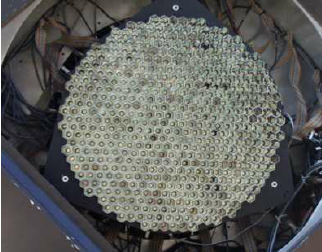
\includegraphics[width=0.6\columnwidth]{figures/verc.png}

        \caption{
                \label{fig:verc} 
                The VERITAS camera design, taken from \cite{vercam}. Note the use of Winston cones to cover the complete focal plane, needed due to the conventional photomultipliers used.
        }
        \end{center}
\end{figure}


\section{Simulations}
The first issue that we contend with in this section is choice of training dataset; which also encompasses choices regarding image cleaning and data pre-selection cuts. The training data should resemble the real observations as closely as possible, but there is a computational trade off between using run-wise simulations (which match the particular set of observations as closely as possible) and completely diffuse training data. All previous attempts at using CNN-based methods have relied upon using tailcut-cleaned images \cite{Shilon} for both the simulated training data and the real test data. We consider this to be counter-productive for background rejection \footnote{This may not be the case for directional reconstruction studies, in which CNNs appear very promising}, despite the fact this procedure simplifies the real observations problem (as it removes the need to accuracy model an entire image with for example 499 pixels vs $\sim$8). Our reasoning for considering tailcut cleaning unhelpful is that the purpose of investigating CNNs for $\gamma$/hadron separation is to utilise their sensitivity to minute features in the air shower images. These small features, such as hadronic halos \cite{model++} (Cherenkov light from the incident primary charged hadron) or subtle electromagnetic substructure would be removed by tailcut cleaning. As such, whilst using it may provide comparable results to BDTs on bright sources such as PKS 2155-304 \cite{Shilon}, using tailcut cleaning partially defeats the purpose of using CNNs for background rejection. Methods reliant upon such cleaning are unlikely to provide a sufficient increase in performance to justify the high computational cost of deep learning techniques.

Whilst there is a large amount of literature available on the problem of domain adaptation \cite{ada}, we believe that part of the key to the success of applying ConvLSTM methods to data will be a partial run wise simulation approach in order to minimise the differences between simulations we use for training and real observations. This is a new paradigm in $\gamma$-ray astronomy \cite{rws}, pioneered by the H.E.S.S. collaboration, and entails generating a unique simulation dataset for every run (28 minutes for H.E.S.S., 20 or 30 minutes for VERITAS) of data collection. The notable achievements of this strategy include the detection of the extension of Centaurus A by an IACT \cite{cena}. However, the VERITAS simulation chain is limited in its ability to reproduce as many run wise effects as H.E.S.S., though we aim to reproduce this approach as much as possible. These simulations were generated using the \textit{CORSIKA} and \textit{CARE} \cite{CARE} simulation packages. \textit{CARE} fulfils the same role in VERITAS as \textit{sim\_telarray} does in CTA and H.E.S.S..

\subsection{Magnetic Field Effects}
In the following subsections we will discuss specific elements of the simulations we utilised. Because of the Lorentz force, and the comparatively strong geomagnetic field at the VERITAS site \cite{kraus}, VERITAS shower images are broadened in differing directions as a function of azimuth. This magnetic field has an overall magnitude of 47 $\mu$T, but the effect of this is is dependent upon the angle between the shower and magnetic field, so only a component of this has an effect on the shower morphology.  To account for this, we match the altitude and azimuth of the simulations to the mean run values in Table \ref{table:obssummary}, with a 5 degree opening angle for both the simulated $\gamma$-rays and protons.

\subsection{Energy Thresholds}
As with all new techniques, the energy thresholds for \textit{CORSIKA} simulations that should be used when attempting to apply deep learning methods to real observations must be determined iteratively. Set the energy threshold too low, and the classifier will struggle to converge on training data (particularly for proton showers which produce relatively little Cherenkov light as a function of energy). But set it too high, and you might loose an improvement in sensitivity at low energies that CNN-type methods might bring. We concluded that using a \textit{CORSIKA} energy range of 100 GeV-200TeV for the $\gamma$-ray simulations, and 300GeV-600TeV for the proton simulations was appropriate (this was after achieving poor results with a lower energy threshold of 30GeV for both protons and $\gamma$-rays).

\subsection{Energy Spectrum and Event Ratios}
Throughout the work in Chapter \ref{ch:3-TimingInfo}, and through our initial investigations into real observations, we have been using simulations with power law spectra and equal ratios of events (albeit over differing energy ranges). It may be argued that this source model is overly simplistic for our purposes. Firstly, not every $\gamma$-ray source on the sky is equally bright, so the ratio of $\gamma$-ray to proton events will not be the same for every observation. Secondly, the spectra both of astrophysical gamma-ray sources and of the cosmic ray background is not a straight power law. This results in an energy dependence in the ratio of gamma-ray to proton events. Thirdly, there is a dependence on low-level trigger selection cuts, if data is only stored for events that produce a certain amount of Cherenkov light then this affects the ratio of stored $\gamma$-rays to stored protons. However, a counterargument to this is that with fewer events at a given energy the ConvLSTM will train less well; and there is a trade off to be had between training efficiency and resembling real observations closely. As such, in this chapter we attempt to balance these effects, and use the VERITAS standard -1.5 spectral index for the training data. Given the ratio of events after basic event pre-selection is approximately 1:1 for the Crab Nebula, we use this as our event ratio in our training data.

\section{Gammaness Cut Optimisation}
Gammaness ($\Gamma$) is the score given to a given event representing how closely the event resembles a $\gamma$-ray. In the \textit{Eventdisplay} framework this is a float in the range [-0.5,0.5]. Typically one discards events from the analysis which have a $\Gamma$ below a particular value, which has to be optimised for the source flux in question. 

Our 2DConvLSTM produces a vector (\textbf{x}) containing two values (one for each event class,   $\textbf{x}_1$ for $\gamma$-rays $\textbf{x}_0$ for protons). The values in this vector span the range [0,1] and must sum to 1. From this, we can construct a $\Gamma$ score through:

\begin{algorithmic}
    \IF{$argmax(\textbf{x}$)=0} 
    \STATE $\Gamma=0.5-\textbf{x}_0$
    \ELSE
    \STATE $\Gamma=\textbf{x}_1-0.5$
    \ENDIF
\end{algorithmic}
There is a question as to how meaningful this particular score is, and the role to which model uncertainty might play. We discuss the possibility for future Bayesian Neural Network analysis in Chapter \ref{ch6-Conclusions}.

For conventional BDT analysis methods, the choice of $\Gamma$ cutoff is optimised to maximise the signal-to-noise ratio for a source. However, this algorithm is known to be difficult to translate to deep learning methods, details of this issue can be found in \cite{Shilon}. For the purposes of our work in this chapter we simply pick a $\Gamma$ value of 0.2.

\section{The Crab Nebula}
The Crab Nebula was the first astrophysical $\gamma$-ray source reliably detected from the ground, in 1989 by the Whipple Observatory \cite{weekestev}. This was due to a mixture of advances in Cherenkov camera technology and the advent of early Hillas analysis for background rejection. \cite{hillasparams}, Earlier `detections' largely relied upon pulsar folding methods that have since been found to be incorrect \cite{paulathesis}, partly as they were limited by camera technology at the time. As a result, the Crab Nebula is one of the most extensively studied $\gamma$-ray objects, and has recently been found to be extended at IACT energies \cite{holler}. In 2019, it was found by the Tibet AS-$\gamma$ experiment that the Crab Nebula produced some of the highest energy photons ever detected, resulting in a 5$\sigma$ detection of the Nebula at over 100TeV \cite{asgamma}. These reasons make the Crab Nebula our first analysis target. Though there are a number of complications associated with this, particularly the greater number of bright stars in the camera field.

\section{Methods}
\subsection{Our Analysis Framework}
Our framework to bootstrap the \textit{Eventdisplay} analysis chain consists of three main steps:

\begin{itemize}
    \item HDF5 file dumpers to convert both simulated and real VERITAS images in .root DST files into a format suitable for deep learning. This includes image mapping and mixing of proton/$\gamma$-ray simulations as appropriate. To obtain data from the root DSTs we use the \textit{root\_numpy} \cite{rootnumpy} package.
    \item \textit{Keras} scripts to perform training and testing of the ConvLSTMs, and write test predictions for a given event to file.
    \item Scripts to take a .root file generated using the normal analysis chain and add an additional tree containing the ConvLSTM predictions in order to make spectra and skymaps.
\end{itemize}

The analysis structure for performing this is shown in Figure \ref{fig:Gettingout}, and the associated code can be found at \url{https://github.com/STSpencer/Getout}. Modifications to the \textit{Eventdisplay} code were also necessary in order to handle both the new deep learning results and the use of run-wise simulations. A significant complicating factor was matching exactly the same number of predictions with the number of events in the data .root files. This mandated testing events individually with a batch size of 1, which slowed the deep learning analysis. A future sufficiently flexible end to end CTA pipeline would avoid this step; we discuss the potential for this in Chapter \ref{ch6-Conclusions}.
\begin{figure}[h] 
        % read manual to see what [ht] means and for other possible options
        \centering 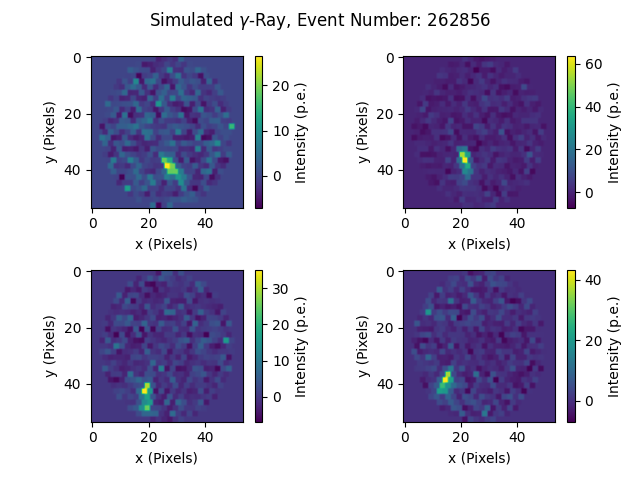
\includegraphics[width=0.8\columnwidth]{figures/sim_272_oversampling.png}

        \caption{
                \label{fig:sim} A simulated VERITAS MC $\gamma$-ray imaged using the oversampling technique. This event is shown as input to the ConvLSTM2D, without image cleaning applied.
        }
\end{figure}
\begin{figure}[h] 
        % read manual to see what [ht] means and for other possible options
        \centering 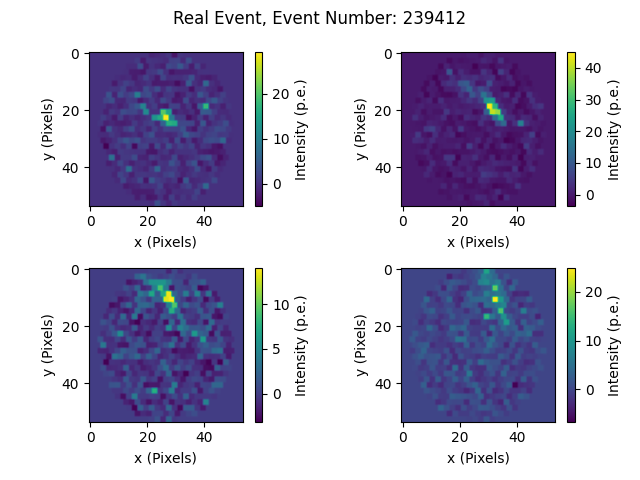
\includegraphics[width=0.8\columnwidth]{figures/realevent_303_oversampling.png}

        \caption{
                \label{fig:real} For comparison with Figure \ref{fig:sim}, a real VERITAS event from run 64080, for which there is no ground truth available. Note that the detector electronics is simulated whereas realistic NSB is not.
        }
\end{figure}
\begin{figure}[t!] 
        % read manual to see what [ht] means and for other possible options
        \centering 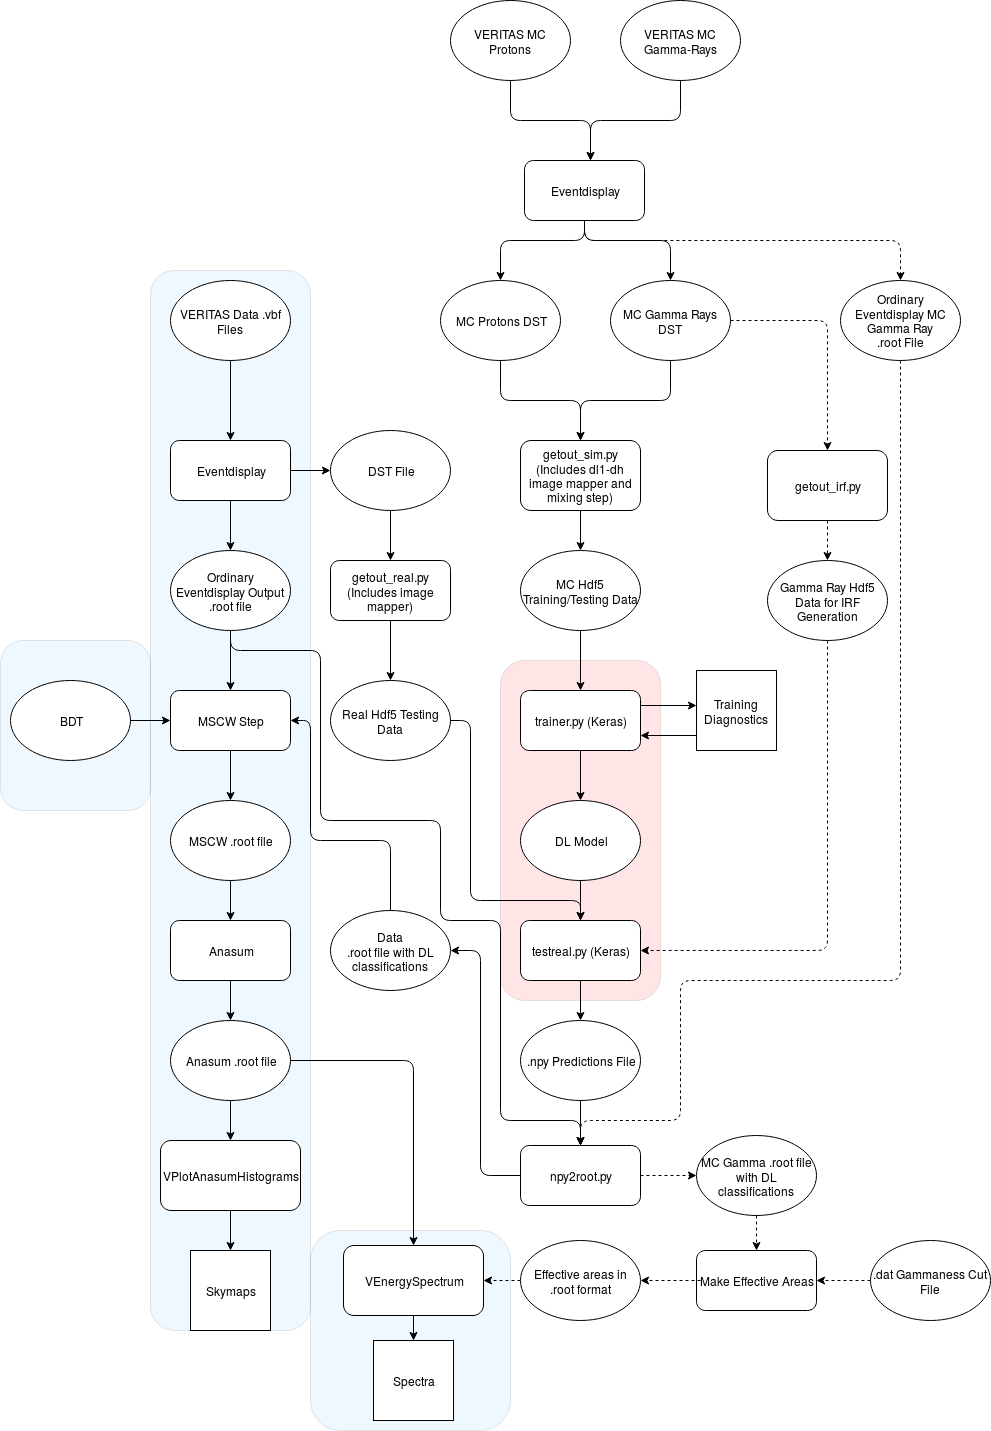
\includegraphics[width=0.83\columnwidth]{figures/Gettingout.png}

        \caption{
                \label{fig:Gettingout} The analysis pipeline I have created in order to perform CNN-based event classification using the VERITAS array. Rectangles represent analysis scripts whereas ellipses represent stored data and squares output products. In the shaded blue region is the standard Eventdisplay pipelines, and on the right is the CNN classification pipeline. The shaded red region indicates code that was run on our group's Nvidia 1080Ti GPU in Oxford, for which there are associated transfer steps in order to relay this information to the computing cluster at DESY. The dashed lines show the pipeline for creation of Effective Areas. The only step not currently implemented is the generation of spectra.
        }
\end{figure}

%This is crabrun2b
\subsection{Effective Areas}
 Effective areas represent the collection area of the IACT array as a function of energy ($E$), and are necessary to generate astrophysical spectra. Our pipeline can generate effective areas, and this gives us an idea of how well our event classifier performs as a function of energy.  They are derived from a $\Gamma$ cut value and Monte Carlo (MC) simulations of $\gamma$-rays through the formula

\begin{equation}
    A_{eff}(E,\theta,\phi)=A_0\left(\frac{\textrm{Number of }\gamma\textrm{-rays that pass event selection }(E,\theta,\phi)}{\textrm{Total number of }\gamma\textrm{-rays }(E,\theta,\phi)}\right)
\end{equation}

which includes a dependence on zenith ($\theta$) and azimuth ($\phi$) angles and a normalisation constant $A_0$. 

\subsection{Issues with the Standard VERITAS Analysis Approach and Deep Learning}
There were two main complications to performing deep learning analysis with \textit{Eventdisplay}. Firstly, VERITAS does not normally use proton air shower simulations, and instead normally operates using BDTs trained on simulated gamma-rays with real proton air shower data as background. This is for reasons of speed, and because of the difficulty of simulating hadronic EAS.  This approach is detailed in \cite{kraus}. In our case for this purpose we utilised observations of the Tycho supernova remnant (not expected to contain a significant number of $\gamma$-rays) with loose Hillas parameter cuts. Early in this investigation we found that this was not going to be a viable approach for CNN-type background rejection methods as the ConvLSTM2D classifier was sufficiently sensitive to be able to determine with 100 percent efficiency the differences between simulated gammas and real proton air showers in training data. When applied to real test data this classifier was no better than a random number generator. As such, we resorted to using proton simulations as training data, in contrast to standard VERITAS operating procedure. Pre-trained BDTs trained with a different, more standard training sample (with simulated $\gamma$-rays and real protons) are supplied with \textit{Eventdisplay}.

Secondly, the VERITAS analysis pipeline is not sufficiently flexible to support the generation of spectra from effective areas produced using our custom simulation approach. Though these effective areas themselves give us some idea of the classifier performance as a function of energy, albeit only on simulated data.

\subsection{Analysis Cuts}
One of the known issues with deep learning research for IACTs is that one needs to be wary of the effect of event pre-selection cuts. These can make it appear as if deep learning methods are performing roughly as well as conventional BDT/RF analysis. However, in such instances all the effective classification power comes from the cuts selected, and the deep learning classifier is acting as a random number generator due to the previously discussed discrepancies with simulated data. Performing harsh pre-selection cuts on training data (using either Hillas parameters or total intensity of images) will improve the AUC values obtained on simulations, but restricting ourselves to such obvious cases of $\gamma$-hadron separation again defeats the purpose of using CNN-based methods. If the only events we consider are events a BDT would easily be able to classify, then there is no potential benefit of using a CNN given their significant complexity and high computational cost. As such, we use minimal dataset cuts throughout this work. We perform no cuts on training data, and only minimal cuts on the MSCW and MSCL (to remove obviously hadronic events) as well as a necessary Theta-Squared cut of 0.008 deg$^2$ that are a default part of the \textit{Eventdisplay} analysis chain on real observations. The cuts used are described in listing \ref{verb1} in Appendix \ref{app:1-VERITASCut}.

\section{Initial Results}
\subsection{Run Summaries}
We began our investigations by selecting which data to replicate. Run 64080 was selected for our investigation due to its high degree of prior investigation and stability, and clear (category A) weather conditions. The observing conditions for this run are summarised in Table \ref{table:obssummary}.
\begin{table}[h]
    \centering
    \resizebox{0.5\textwidth}{!}{
    \begin{tabular}{c|c}
    \textbf{Run Parameter} & Value\\
    \hline
    \textbf{Run Type} & Observing\\
    \textbf{Weather} & A\\
    \textbf{Run Start} & 2012-10-13 10:52:08\\
    \textbf{Observation Mode} & Wobble\\
    \textbf{Offset (RA, DEC)} & (0,0.5)\\
    \textbf{Participating Telescopes} & T1 T2 T3 T4\\
    \textbf{Number of Events} & 543481 \\
    \textbf{Elapsed Time L3 (seconds)} & 1201.8 \\
    \textbf{Live Time L3 (seconds) } & 1013.2 (84.32\%)\\
    \textbf{Mean Trigger Rate (Hz)} & 536.3\\
    \textbf{Mean Elevation (deg)} & 78.86\\
    \textbf{Mean RA, DEC (deg)}& (83.64,22.52)\\
    \end{tabular}
    }
    \caption{Observing summary for run 64080}
    \label{table:obssummary}
\end{table}

\subsection{Effect of Custom Simulations}
The following three figures show the initial results from the use of this pipeline and the custom simulations alone. The neural network was not completely optimised on simulations, scoring an 83\% test accuracy and a 0.91 AUC (good results given the lack of event selection in the simulation test data). But the initial results on the real Crab data were poor, perhaps this was to be expected given the weak cuts and lack of image cleaning used in comparison to the Shilon et al. work \cite{Shilon}. In particular, it should also be noted that most of the background rejection in these results is due to a cut on the theta squared Hillas parameter necessary to perform a reflected region analysis. Despite our initial detection being a ~$7.9\sigma$ detection of the Crab Nebula (which includes very soft cuts on the MSCW and MSCL), a standard BDT analysis gives a ~$22\sigma$ detection and the cut on the MSCW and MSCL alone yields a ~$7.4\sigma$ detection. Evidence for the need for a more thorough analysis of the  uncertainty in the model predictions was demonstrated by the significance not changing if a cut on $\Gamma$ is changed from 0.2 to 0.4.
\begin{table}[h]
    \centering
    \resizebox{\textwidth}{!}{
    \begin{tabular}{c|c|c|c|c|c|c}
    \textbf{Run} & $\textbf{N}_{on}$ & $\textbf{N}_{off}$ & \textbf{Significance} & \textbf{Signal Rate} & \textbf{Error on Signal Rate} & \textbf{Background Rate} \\
    & (events)&(events) & ($\sigma$) & ($\gamma$/min) & ($\gamma$/min) &( events/min) \\
    \hline
    64080 &  175 & 89.17 &   7.3 & 4.285   &0.688 & 4.451\\
    \end{tabular}
    }
    \caption{Anasum output for custom simulations alone run.}
    \label{table:RNG}
\end{table}

\begin{figure}[ht] 
        % read manual to see what [ht] means and for other possible options
        \centering 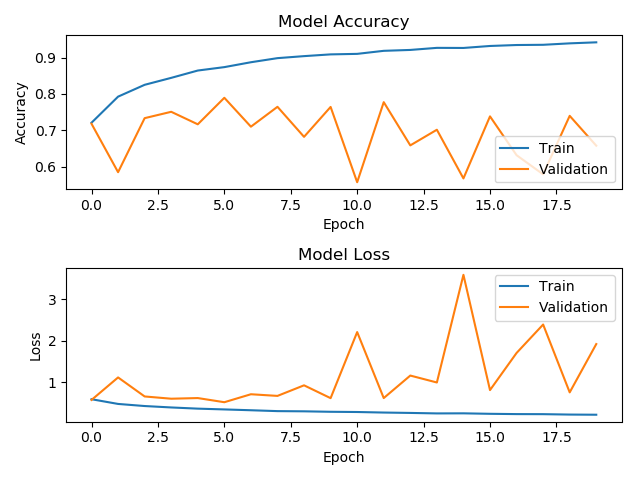
\includegraphics[width=\columnwidth]{figures/crabrun2trainlog.png}

        \caption{
                \label{fig:cr2_trainlog} The training curve for the custom simulation alone run.
        }
\end{figure}

\begin{figure}[ht] 
        % read manual to see what [ht] means and for other possible options
        \centering 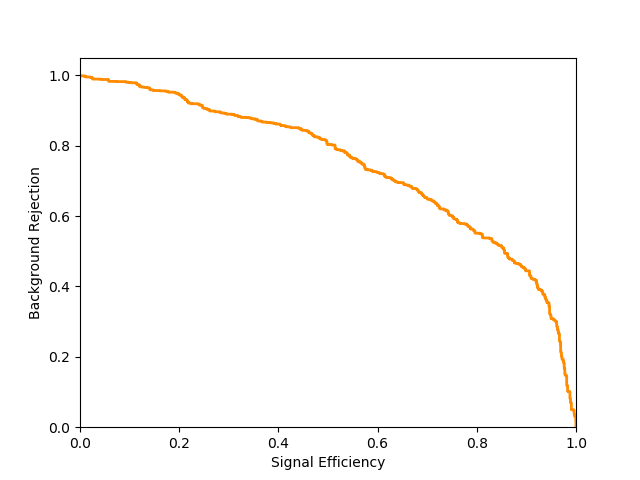
\includegraphics[width=\columnwidth]{figures/crabrun2_sigeff.png}

        \caption{
                \label{fig:cr2_sigeff} The test signal efficiency curve for the custom simulation alone run.
        }
\end{figure}

\begin{figure}[ht] 
        % read manual to see what [ht] means and for other possible options
        \centering \includegraphics[width=\columnwidth]{figures/crabrun2_hist.png}

        \caption{
                \label{fig:cr2_hist} The test gammaness histogram for the custom simulation alone run. The model shows poor convergence on validation data.
        }
\end{figure}

\begin{figure}[h] 
        % read manual to see what [ht] means and for other possible options
        \centering \includegraphics[width=\columnwidth]{figures/skysig.png}

        \caption{
                \label{fig:skysig} A $\gamma$-ray image of the Crab Nebula produced using the initial configuration, custom simulations and our analysis pipeline and our ConvLSTM background rejection technique along with a reflected region analysis. Regions containing bright stars recorded by the HIPPARCOS survey are also shown. Source and excluded regions are shown in purple.
        }
\end{figure}
\begin{figure}[h] 
        % read manual to see what [ht] means and for other possible options
        \centering \includegraphics[width=\columnwidth]{figures/sig1d.png}

        \caption{
                \label{fig:sig1D} The 1 dimensional significance distribution including the source region (Red) and excluding it (Blue) and a Gaussian fit to the cosmic ray background (Green). Significances in IACT $\gamma$-ray astronomy are defined by \cite{LiMa}.
        }
\end{figure}
It appears as though custom simulations (as they are achievable with VERITAS) on their own are not enough to bridge the domain gap between real IACT data and simulations. The poor, noisy performance on validation data throughout the training process is a common feature we observed in using these ConvLSTM2D methods, and is part of the reason we did not use such data in Chapter \ref{ch:3-TimingInfo}. We will find that hyperparameter selection is an important element of this, but we could also be observing a result of the small batch sizes needed to fit such models onto GPUs with finite VRAM.

\subsection{Hillas Width Analysis}
There is a legitimate question of how closely the proton simulations described earlier in this chapter match the real observations and the $\gamma$-ray simulations. If the proton simulations have major discrepancies against the real observations, and if the proton simulations are not reasonably similar to the $\gamma$-ray simulations, this may cause issues with the classifier network. As a control, we retrofit the \textit{ctapipe} Hillas extractor to extract Hillas widths from our VERITAS images for the four telescopes (CT1-4), to act on both our simulated data and the real event images (after disabled pixel interpolation).
\begin{figure}[ht] 
        % read manual to see what [ht] means and for other possible options
        \centering \includegraphics[width=\columnwidth]{figures/Gamma2_int.png}

        \caption{
                \label{fig:Gamma2_int} Hillas Width Distribution for the Simulated $\gamma$-rays for the four telescopes.
        }
\end{figure}
\begin{figure}[ht] 
        % read manual to see what [ht] means and for other possible options
        \centering \includegraphics[width=\columnwidth]{figures/Proton2_int.png}

        \caption{
                \label{fig:Proton2_int} Hillas Width Distribution for the Simulated Protons.
        }
\end{figure}

\begin{figure}[ht] 
        % read manual to see what [ht] means and for other possible options
        \centering \includegraphics[width=\columnwidth]{figures/Real_int.png}

        \caption{
                \label{fig:Real_int} Hillas Width Distribution for the Real Events (Run 64080). 
        }
\end{figure}

The results from this investigation are shown in Figures \ref{fig:Gamma2_int} \ref{fig:Proton2_int} \ref{fig:Real_int}, and we show these results averaged by telescope and normalised such that the distributions integrate to unity in \ref{fig:telaveragedwidth}. All three width distributions are of similar shape with close peak values, suggesting our simulation choice was sound. There are more events for the real data in Figure \ref{fig:Real_int} here due to a \textit{ctapipe} feature that cuts off the analysis if the Hillas parameter extraction fails for the first telescope. The reason for the per telescope discrepancies in distributions in the real observations in Figure \ref{fig:Real_int} is because the real data contains both proton and $\gamma$-ray events; a similar per-telescope discrepancy can be seen in the simulated $\gamma$-rays in Figure \ref{fig:Gamma2_int}. The total number of training events for the ConvLSTM analysis and the real observations are unaffected by this.
\begin{figure}[ht] 
        % read manual to see what [ht] means and for other possible options
        \centering \includegraphics[width=\columnwidth]{figures/telaveragedwidth.png}

        \caption{
                \label{fig:telaveragedwidth} For ease of comparison, the telescope-averaged Hillas width distribution for the simulated proton, $\gamma$-ray and real events from Run 64080, normalised such that the distributions integrate to unity. The real observations appears to be marginally wider than the simulations, this is likely a limit of the hadronic interaction modelling in CORSIKA.
        }
\end{figure}
\subsection{Bayesian Optimisation}
As it is recognised that hyperparameter selection can have a significant effect, we began to consider hyperparameter optimisation. Hyperparameter optimisation is broadly defined as determining $x^*$, the set of hyperparameters that maximize the objective (minimise the loss) function ($f(x)$) of a machine learning algorithm on  data $x$ \begin{equation}
    x^*=\arg \min_{x \in \chi} f(x)
\end{equation}
where $x$ is in a space $\chi$.

One of the most common approaches to hyperparameter optimisation is Bayesian optimisation, and in particular the Tree Parzen Estimator (TPE) approach \cite{bergestra} \cite{tdshyper}. Alternatives include evolutionary- (designed to mimic genetic mutation) and gradient-based approaches, we briefly consider the potential for these methods in Chapter \ref{ch6-Conclusions}. One of the key advantages of this method, unlike other Bayesian optimisation approaches (such as Gaussian processes), is that it is not necessary to specify a Bayesian prior in advance of the analysis. This is well suited to deep learning analysis as the effect of the hyperparameters of a CNN are not always directly human-interpretable. Additionally, one wants the results of prior trials to inform the future searches (formally referred to as Sequential Model Based optimisation), which is not possible with random and grid search techniques \cite{tdshyper}. Leveraging this, TPE optimisers have been shown to be substantially more effective than random searches on standard computer science datasets \cite{bergestra}. Where $y$ is the value of the objective function for a given set of hyperparameters $x^*$, the expected improvement $\textrm{EI}$ (which we aim to maximize at each step) is given by
\begin{equation}
    \textrm{EI}_{y^*}(x^*)=\int_{-\infty}^{y^*}(y^*-y)p(y|x^*)dy
\end{equation}
where $y^*$ is a threshold value of the objective function (below which $p(y|x^*)$ is zero), then TPE models construct a surrogate ($p(x^*|y)$) for the objective function indirectly using Bayes' rule
\begin{equation}
    p(y|x^*)=\frac{p(x^*|y)*p(y)}{p(x^*)}
\end{equation}
which is the probability of the hyperparameters given the score on the objective function \cite{tdshyper}. In turn, this surrogate is modelled as two separate distributions by TPE methods

\begin{equation}
    p(x^*|y) = \begin{cases} \textit{l}(x^*) & \mbox{, if }  y <y^* \\ \textit{g}(x^*) & \mbox{, if } y>=y^* \end{cases}
\end{equation}

where $y^*$ is the threshold value of the objective function. Using Bayes' theorem and substitution, the $\textrm{EI}$ can then be written (introducing a constant value $\gamma$) as 
\begin{equation}
    \textrm{EI}_{y^*}(x^*)=\frac{\gamma y^* \textit{l}(x^*)-\textit{l}(x^*)\int_{-\infty}^{y^*}p(y)dy}{\gamma \textit{l}(x^*)+(1-\gamma) \textit{g}(x^*)} \propto \left( \gamma +\frac{\textit{g}(x^*)}{\textit{l}(x)} (1-\gamma)\right)^{-1}
\end{equation}


The TPE approach then maximises the $\textrm{EI}$ by drawing values from $\textit{l}(x^*)$, and maximizing the ratio $\textit{l}(x^*)/\textit{g}(x^*)$, which in term maximises the $\textrm{EI}$ \cite{tdshyper}. In practice, the fact that the surrogate is not exactly the objective may mean that the hyperparameter choice offers no improvement in the objective. Therefore the surrogate function needs to be updated, and the use of a distribution $\textit{l}(x^*)$ helps to balance the trade-off between exploration and exploitation. In practical terms, this can reasonably be thought of as performing gradient descent over hyperparameter values, with the loss function as the quantity being optimised.

\subsection{Initial Optimisation Efforts}

To investigate the potential of Bayesian optimisation, we utilized the \textit{Hyperas} \cite{hyperas} \textit{Keras} wrapper around \textit{Hyperopt} \cite{hyperopt}. This is one of the most commonly-used Python packages for performing TPE analysis. However, given that this approach requires (at least partially) training a classifier for every point in hyperparameter space explored. This process is orders of magnitude more computationally costly than simply training a single deep learning classifier with a single hyperparameter configuration. It was also not immediately clear what the best approach to take with these methods given realistically finite compute power and time. There is a choice between the number of epochs to train a model for each point in hyperparameter space, the amount of data used for training and the number and range of hyperparameter space points probed. The optimal configuration for this was not known at the starting point of this research. In practice, VRAM constraints limit the maximum possible range of hyperparameter values probed. Extending this range too far, for example in terms of number of layers, will eventually exhaust finite VRAM and cause crashes.

\begin{figure}[] 
        % read manual to see what [ht] means and for other possible options
        \centering \includegraphics[width=\columnwidth]{figures/EFF.png}

        \caption{
                \label{fig:EFF} Effective area of VERITAS as a function of energy, made using our analysis pipeline and the opt4 configuration. This shows performance broadly similar to BDTs on simulations, see for comparison \cite{vereff}. However, it does not show a substantial improvement. This could likely be an effect of the custom simulation approach we use. The parameters for this are as follows: Zenith angle $10^{\circ}$, wobble offset=$0.5^{\circ}$, $\gamma$-ray spectral index=-1.5, noise level=250Hz. 
        }
\end{figure}
The initial optimisation efforts revolved around training a ConvLSTM2D classifier for a single epoch on a comparatively small number of events ($\sim$19574 simulated events) on a single GPU, using performance on a similarly small amount of validation data as a metric. The hyperparameter space for this optimisation is shown in Table \ref{table:runsopt4}, where we use hyperopt convention to define the hyperparameter space. For example, Choice() represents optimising a discrete choice between a finite number of options (this can include binary selection such as the inclusion of layers, as well as selection between two dimensional objects like filter sizes) and Uniform() means the value can take any float value in a given range. The aim was to find the best `starting position' for the training. The network configuration generated following the initial hyperopt run was then trained for 100 epochs with the complete training dataset (235174 events in total). This resulted in the 'opt4' configuration presented here, yielding performance superior to random number generation on the real observations. This detection represents the first time the Crab nebula has been detected with an IACT array using a deep-learning-based event classification method, and was the first deep-learning-based detection not to rely upon image cleaning.

\begin{table}[ht]
    \centering
    \resizebox{\textwidth}{!}{
    \begin{tabular}{ccc|c|c|c}
    \textbf{Block} & \textbf{Layer} & \textbf{Parameter} & \textbf{Potential Values}& \textbf{Optimal Value Diffuse Source} \\
    \hline
    \hline
    \textbf{Block 1} & ConvLSTM2D & Number of Filters & Choice(10,20,30,40) &  10 \\
                     &            & Kernel Size & Choice((2,2),(3, 3),(4,4),(5,5)) & (4,4) \\
                     &            & Kernel L2 Regularizer Rate & Uniform(0,1) & 0.0797 \\
                     &            & Dropout Rate & Uniform(0,1) &  0.0361 \\
                     &            & Recurrent Dropout Rate & Uniform(0,1) & 0.382 \\
    \hline
    \textbf{Block 2} & ConvLSTM2D & Number of Filters & Choice(10,20,30,40) & 10 \\
                     &            & Kernel Size & Choice((2,2),(3, 3),(4,4),(5,5)) &  (2,2) \\
                     &            & Kernel L2 Regularizer Rate & Uniform(0,1) & 0.576 \\
                     &            & Dropout Rate & Uniform(0,1) & 0.371 \\
                     &            & Recurrent Dropout Rate & Uniform(0,1) & 0.510 \\
    \hline
    \textbf{Block 3} & ConvLSTM2D & Number of Filters & Choice(10,20,30,40) & 40 \\
                     &            & Kernel Size & Choice((2,2),(3, 3),(4,4),(5,5) & (2,2) \\
                     &            & Dropout Rate & Uniform(0,1) & 0.0 \\
                     &            & Recurrent Dropout Rate & Uniform(0,1) & 0.1 \\
    \hline
    \textbf{Block 4} &.           & Include Block & Choice(Yes,No)                      & Yes \\
                     & ConvLSTM2D & Number of Filters & Choice(10,20,30,40) &  30 \\
                     &            & Kernel Size & Choice((2,2),(3, 3),(4,4),(5,5))  & (5,5) \\
                     &            & Dropout Rate & Uniform(0,1) &  0.5056 &\\
    \hline
    \textbf{Block 5} & GlobalAveragePooling3D &  - & - &- \\
    \hline
    \textbf{Block 7} & Dense      & Number of Units & Choice(10,50,100,200) & 100 \\
    \hline
    \textbf{Block 8} & Dense      & - & - & - \\


    \end{tabular}
    }
    \caption{Summary of hyperparameter space and selected configuration for the initial single core optimisation that produced the opt4 configuration.}
    \label{table:runsopt4}
\end{table}
\begin{table}[h]
    \centering
    \resizebox{\textwidth}{!}{
    \begin{tabular}{c|c|c|c|c|c|c}
    \textbf{Run} & $\textbf{N}_{on}$ & $\textbf{N}_{off}$ & \textbf{Significance} & \textbf{Signal Rate} & \textbf{Error on Signal Rate} & \textbf{Background Rate} \\
    & (events) & (events) & ($\sigma$) & ($\gamma$/min) & ($\gamma$/min) & (events/min) \\
    \hline
    64080 &  573 & 280.17 & 13.9 & 14.617  & 1.243 & 13.985\\
    \end{tabular}
    }
    \caption{Anasum output for the opt4 run, without applying a strenuous multiplicity cut.}
    \label{table:opt4}
\end{table}

This significance of this detection is a mild function of multiplicity, the significance can reach 16.1 $\sigma$ if a telescope multiplicity cut of 4 is imposed, this is a result of the signal-to-noise ratio being higher for such events. The standard VERITAS analysis, reliant upon BDTs, achieves a 21 $\sigma$ detection on the same data without this strong multiplicity cut, although it is trained with a different dataset so the comparison is imperfect. \footnote{Details of this analysis can be found at \url{https://veritas.sao.arizona.edu/wiki/index.php/Eventdisplay_Manual:_event_display}; but not that this is a VERITAS internal site only accessible from VERITAS member institutes.}

\begin{figure}[h] 
        % read manual to see what [ht] means and for other possible options
        \centering \includegraphics[width=\columnwidth]{figures/crabrun2opt4trainlog.png}

        \caption{
                \label{fig:opt4_trainlog} The training curve for the opt4 run.
        }
\end{figure}

Curiously the validation data training curve appears to converge in this one specific instance, but it is unclear if this relates to the ConvLSTM2D classifier learning meaningful features in the simulated images or if this is simply a coincidence. 

\begin{figure}[ht] 
        % read manual to see what [ht] means and for other possible options
        \centering \includegraphics[width=\columnwidth]{figures/crabrun2opt4_sigeff.png}

        \caption{
                \label{fig:opt4_sigeff} The test signal efficiency curve for the opt4 run.
        }
\end{figure}

\begin{figure}[ht] 
        % read manual to see what [ht] means and for other possible options
        \centering \includegraphics[width=\columnwidth]{figures/crabrun2opt4_hist.png}

        \caption{
                \label{fig:opt4_hist} The test gammaness histogram for the opt4 run.
        }
\end{figure}
\begin{figure}[ht] 
        % read manual to see what [ht] means and for other possible options
        \centering \includegraphics[width=\columnwidth]{figures/opt4_skysig.png}

        \caption{
                \label{fig:opt4_skysig} The sky significance for the 'opt4' configuration on run 64080.
        }
\end{figure}
\begin{figure}[ht] 
        % read manual to see what [ht] means and for other possible options
        \centering \includegraphics[width=\columnwidth]{figures/opt4_sig.png}

        \caption{
                \label{fig:opt4_sig1D} The 1 dimensional significance for the 'opt4' configuration on run 64080.
        }
\end{figure}

\section{Parallelised Optimisation Attempts}
\subsection{Optimisation Configurations and Results}
Following our initial success with Bayesian optimisation, we ran extensive further investigations with improved computational power in order to test the performance limit of this new technique. The next three figures and three tables show three attempts to perform Bayesian optimisation using \textit{hyperas} in parallel using the recently upgraded \textit{glamdring} cluster. Four of the machines had two NVidia 2080Tis attached, the final had only one. The machines with multiple GPUs made use of Tensorflow's \textit{MirroredStrategy} approach, so the optimisation worker effectively saw a single GPU with double the VRAM of a 2080Ti. We'll refer to these three optimisation attempts as attempt A, attempt B and attempt C. After each optimisation attempt the best performing model was trained with the complete dataset for more epochs, similar to the earlier strategy on the single GPU. In all attempts, a unique configuration database was created, with each point in hyperparameter space being allocated a unique working directory. To operate, the optimiser consisted of a head process working on the \textit{glamdring} login node to determine hyperparameter point selection, and up to 5 worker processes on the \textit{glamdring} GPU nodes. Progress was checkpointed such that there were no information losses if a worker process failed. The classifier trained on a certain subset of training data for a certain number of epochs for each hyperparameter configuration, and the accuracy on test data after this training was used as the metric. Each of these test scores is shown as a blue cross, running averages and moving averages (over the maximum 9 parallel GPUs) are also shown. Attempt A had a similar hyperparameter space to the initial single core optimisation run that produced the opt4 configuration, albeit using a greater number of training epochs per hyperparameter point. This hyperparameter space was increased for the subsequent attempts B and C. It should be noted that in particular optimisation attempt C, our final attempt to generate a configuration superior to the opt4 result, was extremely computationally intensive (representing the results of around 5800 GPU hours of compute time).

\begin{table}[ht]
    \centering
    \resizebox{\textwidth}{!}{
    \begin{tabular}{c|c|c|c}
    \textbf{Attempt} & \textbf{A} & \textbf{B} & \textbf{C} \\
    \hline
    \textbf{No. Training Events}                       & 39148 & 19574 & 117574 \\
    \textbf{No. Test Events}                           & 39200 & 19600 & 39200 \\
    \textbf{Epochs Training per Hyperparameter Point}  & 5     & 1     & 25 \\
    \textbf{No. Hyperparameter Points Sampled}         & 2000  & 1000  & 500 \\
    \textbf{Best Test Accuracy (\%)}                   & 77.36 & 75.9  & 86.4 \\
    \end{tabular}
    }
    \caption{Summary of parallelised optimisation runs and the amount of data used for each. Values presented here represent the number of training events, test events, and test performance for the training and evaluation during the Bayesian optimisation process. The best performing models from each optimisation run were then trained and tested again with the complete dataset for more epochs before being applied to the real observations.}
    \label{table:optsum}
\end{table}

\begin{table}[ht]
    \centering
    \resizebox{\textwidth}{!}{
    \begin{tabular}{ccc|c|c|c|c}
    \textbf{Block} & \textbf{Layer} & \textbf{Parameter} & \textbf{Potential Values}& \textbf{Optimal Value Attempt A}& \textbf{Optimal Value Attempt B} \\
    \hline
    \hline
    \textbf{Block 1} & ConvLSTM2D & Number of Filters & Choice(10,20,30,40) &  20 & 10\\
                     &            & Kernel Size & Choice((2,2),(3, 3),(4,4),(5,5)) & (4,4)& (4,4) \\
                     &            & Kernel L2 Regularizer Rate & Uniform(0,1) & 0.402 & 0.404 \\
                     &            & Dropout Rate & Uniform(0,1) &  0.462 & 0.536\\
                     &            & Recurrent Dropout Rate & Uniform(0,1) & 0.552& 0.353\\
    \hline
    \textbf{Block 2} & ConvLSTM2D & Number of Filters & Choice(10,20,30,40) & 10& 20\\
                     &            & Kernel Size & Choice((2,2),(3, 3),(4,4),(5,5)) &  (2,2)& (4,4)\\
                     &            & Kernel L2 Regularizer Rate & Uniform(0,1) & 0.234& 0.796\\
                     &            & Dropout Rate & Uniform(0,1) & 0.774& 0.563\\
                     &            & Recurrent Dropout Rate & Uniform(0,1) & 0.000& 0.116\\
    \hline
    \textbf{Block 3} & ConvLSTM2D & Number of Filters & Choice(10,20,30,40) & 30& 30\\
                     &            & Kernel Size & Choice((2,2),(3, 3),(4,4),(5,5) & (2,2)& (4,4) \\
                     &            & Dropout Rate & Uniform(0,1) & 0.444& 0.105\\
    \hline
    \textbf{Block 4} &.           & Include Block & Choice(Yes,No)                      & Yes& Yes \\
                     & ConvLSTM2D & Number of Filters & Choice(10,20,30,40) &  40& 30\\
                     &            & Kernel Size & Choice((2,2),(3, 3),(4,4),(5,5))  & (5,5)& (5,5)\\
                     &            & Dropout Rate & Uniform(0,1) &  0.720 & 0.652\\
    \hline
    \textbf{Block 5} & GlobalAveragePooling3D &  - & - &- &-\\
    \hline
    \textbf{Block 7} & Dense      & Number of Units & Choice(10,50,100,200) & 10 & 100\\
    \hline
    \textbf{Block 8} & Dense      & - & - & - \\


    \end{tabular}
    }
    \caption{Summary of hyperparameter space and selected configuration for the initial parallelised optimisation runs, attempts A and B.}
    \label{table:runsAB}
\end{table}

\begin{table}[ht]
    \centering
    \resizebox{\textwidth}{!}{
    \begin{tabular}{ccc|c|c}
    \textbf{Block} & \textbf{Layer} & \textbf{Parameter} & \textbf{Potential Values} & \textbf{Optimal Value Attempt C} \\
    \hline
    \hline
    \textbf{Block 1} & ConvLSTM2D & Number of Filters & Choice(10,20,30,40,50,60) &  10 \\
                     &            & Kernel Size & Choice((2,2),(3, 3),(4,4),(5,5),(6,6),(7,7)) & (4,4) \\
                     &            & Kernel L2 Regularizer Rate & Uniform(0,1) & 0.366 \\
                     &            & Dropout Rate & Uniform(0,1)  & 0.414 \\
                     &            & Recurrent Dropout Rate & Uniform(0,1) & 0.107 \\
    \hline
    \textbf{Block 2} & ConvLSTM2D & Number of Filters & Choice(10,20,30,40,50,60) & 10 \\
                     &            & Kernel Size & Choice((2,2),(3, 3),(4,4),(5,5),(6,6),(7,7)) &  (2,2) \\
                     &            & Kernel L2 Regularizer Rate & Uniform(0,1) & 0.167 \\
                     &            & Dropout Rate & Uniform(0,1) & 0.863 \\
                     &            & Recurrent Dropout Rate & Uniform(0,1) & 0.321 \\
    \hline
    \textbf{Block 3} & ConvLSTM2D & Number of Filters & Choice(10,20,30,40,50,60) & 40 \\
                     &            & Kernel Size & Choice((2,2),(3, 3),(4,4),(5,5),(6,6),(7,7)) & (2,2) \\
                     &            & Kernel L2 Regularizer Rate & Uniform(0,1) & 0.219 \\
                     &            & Dropout Rate & Uniform(0,1) & 0.287 \\
                     &            & Recurrent Dropout Rate & Uniform(0,1) & 0.697 \\
    \hline
    \textbf{Block 4} & ConvLSTM2D & Number of Filters & Choice(10,20,30,40,50,60) &  30 \\
                     &            & Kernel Size & Choice((2,2),(3, 3),(4,4),(5,5),(6,6),(7,7))  & (3,3) \\
                     &            & Dropout Rate & Uniform(0,1) &  0.483 \\
    \hline
    \textbf{Block 5} &            & Include Block & Choice(Yes, No)                     & Yes \\
                     & ConvLSTM2D & Number of Filters & Choice(10,20,30,40,50,60)  & 30 \\
                     &            & Kernel Size & Choice((2,2),(3, 3),(4,4),(5,5),(6,6),(7,7))  & (3,3) \\
                     &            & Dropout Rate & Uniform(0,1) &  0.020 \\
    \hline
    \textbf{Block 6} &            & Include Block & Choice(Yes, No)                     & Yes \\
                     & ConvLSTM2D & Number of Filters & Choice(10,20,30,40,50,60) &  30 \\
                     &            & Kernel Size & Choice((2,2),(3, 3),(4,4),(5,5),(6,6),(7,7))  & (3,3) \\
                     &            & Dropout Rate & Uniform(0,1) & 0.553 \\
    \hline
    \textbf{Block 5} & GlobalAveragePooling3D &  - & - &- \\
    \hline
    \textbf{Block 6} &            & Include Block & Choice(Yes, No)                     &  Yes \\
                     & Dense      & Number of Units & Choice(10,50,100,200) & 10 \\
                     &            & Dropout Rate & Uniform(0,1) & 0.190 \\
    \hline
    \textbf{Block 7} &            & Include Block & Choice(Yes, No)                     &  Yes \\
                     & Dense      & Number of Units & Choice(10,50,100,200) & 200 \\
                     &            & Dropout Rate & Uniform(0,1) & 0.743 \\
    \hline
    \textbf{Block 8} &            & Include Block & Choice(Yes, No)                     &  Yes \\
                     & Dense      & Number of Units & Choice(10,50,100,200) & 200 \\
                     &            & Dropout Rate & Uniform(0,1) & 0.107 \\
    \hline
    \textbf{Block 9} & Dense      &  - & - \\




    \end{tabular}
    }
    \caption{Summary of hyperparameter space and selected configuration for the final parallelised optimisation run, attempt C.}
    \label{table:runsC}
\end{table}

\begin{figure}[h] 
        % read manual to see what [ht] means and for other possible options
        \centering \includegraphics[width=\columnwidth]{figures/convplot_testfolders3.png}

        \caption{
                \label{fig:convplot_testfolders3} Final test accuracies after  training optimisation for longer Bayesian optimisation run attempt A
        }
\end{figure}
\begin{figure}[h] 
        % read manual to see what [ht] means and for other possible options
        \centering \includegraphics[width=\columnwidth]{figures/convplot_febtry.png}

        \caption{
                \label{fig:convplot_febtry} Final test accuracies after training optimisation for longer Bayesian optimisation run attempt B.
        }
\end{figure}

\begin{figure}[h] 
        % read manual to see what [ht] means and for other possible options
        \centering \includegraphics[width=\columnwidth]{figures/convplot_longmoredata.png}

        \caption{
                \label{fig:convplot_longmoredata} Final test accuracies after training optimisation for Bayesian optimisation attempt C.
        }
\end{figure}

Final simulated data training curves and signal efficiency curves for the best model configuration for optimisation attempt C, trained with the complete dataset are shown in Figures \ref{fig:6vimrcb1485481664_trainlog} and Figure \ref{fig:6vimrcb1485481664_sigeff} for completeness. Whilst none of these attempts generated a model superior to the opt4 configuration, this final optimisation run C is of interest as the running average shows evidence of convergence. This has not often seen with TPE methods, and this is a known issue them \cite{autosklearn}. Notably this is the first attempt at Bayesian optimisation with IACT data to ever see evidence of convergence, let alone with a stereoscopic array \cite{nietopc}. This is likely a result of the large number of epochs, the large amount of data used, and the long period the optimiser was left to run. This combined with the fact we did not achieve performance superior to the opt4 run suggests that the opt4 configuration represents the current limit of what is technically possible with deep learning event classifiers, with this configuration of simulations and cuts.

\begin{figure}[h] 
        % read manual to see what [ht] means and for other possible options
        \centering \includegraphics[width=\columnwidth]{figures/6vimrcb1485481664trainlog.png}

        \caption{
                \label{fig:6vimrcb1485481664_trainlog} Training accuracy curve for the best performing model from optimisation attempt C, trained for 100 epochs with the complete dataset.
        }
\end{figure}

\begin{figure}[h] 
        % read manual to see what [ht] means and for other possible options
        \centering \includegraphics[width=\columnwidth]{figures/6vimrcb1485481664_sigeff.png}

        \caption{Test signal efficiency curve for the best performing model from optimisation attempt C, trained for 100 epochs with the complete dataset.
                \label{fig:6vimrcb1485481664_sigeff} 
        }
\end{figure}


\section{Conclusion}
In this chapter, we have demonstrated a deep learning pipeline capable of use with the VERITAS telescopes, and showed that a combination of ConvLSTM2D classifiers, custom simulations and Bayesian optimisation can yield a definite detection of the Crab Nebula. The is the first detection with an IACT array using such methods that did not require conventional tailcut cleaning. However, there are significant issues with this approach that limit its current efficacy for CTA that require further detailed study. In particular, it is clear that the modelling of NSB used by current generation IACTs is too simplistic for use with deep learning event classification methods for CTA. It is also clear that there is a very significant hyperparameter dependence problem with ConvLSTM2D and similar classifiers which limits their use in practice. It should also be noted that the combination of optimisation and custom simulations we used is likely to be computationally prohibitive in a real observing scenario. Our achieved aim was to determine the maximal possible potential for these deep learning methods, and we performed this work operating under the hope that at some point new transfer learning, optimisation and simulation approaches might be able to bridge the gap in computing power needed. Given these results, it seems likely that in order to fully leverage the potential for deep-learning-based analyses we must either look to new methods of interpretation of IACT data, such as leveraging high precision timing information as presented in Chapter \ref{ch:3-TimingInfo}, or to new deep learning techniques beyond conventional CNNs. That said, it also appears that we have discovered a weak correlation between accuracy on simulated test data and performance on real observations. The pipeline we developed for these purposes could be used in future work for VERITAS should new mitigation strategies become apparent.

Ultimately, as none of the longer, parallelised optimisation runs produced a model that outperformed the opt4 configuration after final training and testing on the whole simulated dataset, combined with the convergence appearing in attempt C's moving average optimisation curve, suggests that we have hit the simulation accuracy limit (87\%) for this selection of cuts and this simulation data. So whilst Bayesian optimisation is a powerful tool that can allow for real detections to be made in IACT data, it cannot be claimed to be consistently reliable. 
\chapter{\label{ch:5-CHECNSB} Advanced Study of SSTCAM NSB}
\minitoc
\section{Introduction}
\label{sec:intro}

\subsection{Scope \& Purpose of this Chapter}
\label{sec:intro:scope}
As we've seen in Chapters \ref{ch:3-TimingInfo} and \ref{ch:4-VERITASRealData}, it is clear that the current modelling of NSB in both the simulation packages \textit{CARE} (used by VERITAS and in Chapter \ref{ch:4-VERITASRealData}) and \textit{sim\_telarray} (used by CTA and H.E.S.S. and in Chapter \ref{ch:3-TimingInfo}) is insufficient to allow for reliable deep-learning-based event classification. In this chapter, we estimate the expected NSB photon rates of SSTCAM under various observing conditions. This modelling will aid SSTCAM design, as well as begin a possible route to improvement in our training data that might one day make deep learning analyses feasible. These investigations have been the subject of an SSTCAM internal note. We perform this by using and expanding upon the capabilities of the \textit{nsb} tool \cite{nsb}, already validated and used by H.E.S.S.. \footnote{For the purposes of this chapter, capitalised NSB refers to the physical phenomenon of Night Sky Background, where as italic lower case \textit{nsb} refers to the Python package used to simulate it.}. Full results from this study, along with sandbox scripts to operate \textit{nsb} can be found on the \url{https://github.com/sstcam/sstcam_NSB} Github page. 

\subsection{Context}
\label{sec:intro:context}
The ability for SSTCAM to operate reliably under partially moonlight and other high NSB observing conditions is critical to the transient and multi-messenger/multi-wavelength science goals of CTA, as it significantly increases the possible observing time. As a result, this ability to operate under moonlit conditions results in a CTA system requirement. The increase in potential science return has been judged to outweigh the associated increase in data rate and person-power required to operate the telescopes. The most notable example for this is the detection of prompt TeV emission from GRB 190114C (the first such detection from the ground), which was detected under partial moonlit (6 times nominal NSB) conditions with MAGIC \cite{magicGRB}. 

Studies of partial moonlight and high NSB observations can also help inform temperature management and SiPM selection for SSTCAM, as well as inform estimations of astrophysical systematic errors. The continuous rate of illumination, analogous to a constant NSB value, across the camera plane affects almost all measurable properties of SiPMs. This is as the bias voltage across the SiPMs is reduced which in turn reduces their sensitivity to light \cite{1mhighnsb}. The majority of previous studies concerning NSB for SiPM-based Cherenkov cameras have primarily focused on NSB's effect on single SiPM pixels \cite{2msipm} \cite{1mcalib} \cite{1mhighnsb} \cite{lstnsb}. The work presented in this chapter is the first detailed simulations of an entire SiPM-based camera's worth of NSB, allowing us to evaluate both the spatial and temporal properties of NSB across the camera plane.

SiPMs are typically operated with a bias circuit with a resistor connected in series, to protect the SiPMs from drawing too much current from the power supply and being damaged. We need to determine the correct bias voltage to set for this system, so we define the overvoltage as $\Delta V=V_{PS}-V_{BD}$, where $V_{BD}$ is the breakdown voltage (the minimum (reverse) bias voltage under which electron avalanche production is possible in an SiPM) and $V_{PS}$ is the bias voltage supplied by the power supply \cite{1mhighnsb}. As a change in NSB rate results in a change of the overvoltage of the SiPMs, which in turn affects the photomultiplier calibration. SSTCAM hopes to counter this with the LED flasher system, and so the rate of change of NSB in the camera affects the number and rate of LED flashes required. We consider the necessary rate of LED flashes to correct for the effects of NSB later in this chapter.
\subsection{Model}
\label{sec:intro:model}

The standard CORSIKA/\textit{sim\_telarray} simulation package \cite{simtel} used for CTA Monte-Carlo simulation productions supports NSB maps as an input parameter, and has some limited functionality to replicate illumination at an infinite distance from the camera (i.e. stars). For reasons of computational efficiency, it does not calculate where in the camera and how bright those stars might be, nor does it realistically simulate the effect of moonlight. We model NSB using the \textit{nsb} package, which assumes that NSB comes from two primary sources. The first is starlight using \textit{Gaia} data, and the second is sky brightness taking account of moonlight and a local extinction coefficient following the semi-analytic model of Krisciunas and Schaeffer \cite{Krisciunas}. The Krisciunas and Schaeffer model was originally fit to data from Mauna Kea before being extended later with additional weight parameters accounting for the relative brightness between the sky and the extra component of starlight in the \textit{hess\_basic} model included in \textit{nsb}. The \textit{hess\_basic} model is expressed as:
\begin{equation}
    f(\rho, A, B, C) = 10^{A}\times (1.06+\cos^2(\rho))+10^{B-\rho/40}+C \times 10^7 \times \rho^2,
\end{equation}

\begin{equation}
    I_{M} (\alpha_{M}) = 10^{-0.4 \times (3.84 + 0.026 \times |\alpha_{M}| + 4 \times 10^{-9} \times \alpha_{M}^4))},
\end{equation}

\begin{equation}
    X(Z)=\begin{cases} (1-0.96\sin^2 Z)^{-0.5} & \mbox{, if }  Z<=\pi/2 \\ (1 - 0.96 \times 1)^{-0.5} & \mbox{, otherwise } \end{cases},
\end{equation}

\begin{equation}
\begin{aligned}
    B_{Moon}(\rho,Z,Z_{M},k,\alpha_{M},A,B,C)=f(\rho,A,B,C) \times I_{M}(\alpha_{M}) \\ \times 10^{-0.4kX(Z_{M})}\\ \times [1-10^{-0.4 k X(Z)}]
\end{aligned}
\end{equation}

\begin{equation}
    B_{Sky}(Z,\phi,B_0,k)=\begin{cases} B_0\times X(Z) \times 10^{-0.4k(X(Z)-1)} & \mbox{, if }  Z<=\pi/2 \\ 0 & \mbox{, otherwise } \end{cases},
\end{equation}

\begin{equation}
    B_{Total}=B_{Moon}+B_{Sky}+B_{Gaia}
\end{equation}

where $B_{Total}$ is the total brightness for a given point on the sky, $B_{Moon}$ is the surface brightness from moonlight, $B_{Sky}$ is the intrinsic surface brightness of the sky, $B_{Gaia}$ is the brightness of stars in the associated healpix pixel \cite{healpix}, $Z$ is the Zenith angle, $\phi$ is the azimuth (with subscript $_M$ referring to Moon parameters rather than source parameters), $f(\rho,A,B,C)$ is the scattering function as a function of lunar great circle separation angle $\rho$ (which takes into account in this form both Rayleigh scattering from atmospheric gases and Mie scattering from atmospheric aerosols), $\alpha_M$ is the phase angle of the Moon and $I_m$ is the illuminance of the Moon in footcandels. $A$,$B$,$C$,$k_0$ and $B_0$ are all free parameters to be determined, values used are in Table \ref{tab:params}. $B_{Total}$ (along with all the other native outputs from the \textit{hess\_basic} \textit{nsb} model) is expressed here in nanoLamberts (nLb), where a brightness in nanoLamberts $B$ relates to magnitudes per square arc second in the V band ($V$) through
\begin{equation}
    \frac{B}{\textrm{nanoLamberts}}=34.08\exp(20.7233-0.92104\times V)
\end{equation}
\cite{Krisciunas}.

The stellar data in \textit{nsb} is obtained using \textit{dr1b} stellar magnitude data from the \textit{Gaia} space mission \cite{gaiadr1a}\cite{gaiadr1b}. Understanding the behaviour of the SiPMs under the illumination of a particularly bright star is important for the future operation plan of SSTCAM. Current practice of most previous Cherenkov cameras is turning the high voltage of blocks of pixels containing such bright stars off. SSTCAM will not have to do this as saturating SiPMs is more tolerable than with them than conventional photomultipliers. If we choose to alter bias voltage for such pixels, it may be adjusted pre-emptively or as a reaction; this is further complicated by the need to use such stars for the slow signal pointing calibration simultaneously. 

Given lack of data from an SSTCAM prototype on the Paranal site it is currently not possible to fit the relative coefficients of the stellar and semi-analytic components of the model. Given the coefficients from HESS and Mauna Kea were within 10\%, we can accept the HESS values as placeholders in the expectation that, if anything, Cerro Paranal will offer superior observing conditions. It should also be noted that the \textit{nsb} package does not explicitly take into account certain other known sources of NSB, in particular contributions from zodiacal light, light from population centres (particularly from mines near $\sim$ 25 km from the Cerro Paranal site \cite{cpmines}), stray reflections from the ground, light from satellites (the \textit{Starlink} satellite is of particular concern, with the satellites reaching $\mathrm{m_G=2.4}$ during the deployment phase, though this decreases to $\mathrm{m_G=6.6}$ afterwards \cite{starlink}) and air glow emission lines in the atmosphere (see Figure \ref{fig:BandE} \cite{BandE}, though these are smaller effects compared to the differences between full moonlight illumination and astronomical dark time. A rough calculation using the spectrum from \cite{BandE} shows that air glow emission lines contribute to a constant NSB value of around 17MHz by themselves in the SSTCAM wavelength range, primarily from the OI 5577\r{A} and Na D 5890\r{A} lines (utilising the standard \cite{BandE} measurements from La Palma). Also not considered here is the potential effect of the 8 magnitude 6.8 laser guide stars used by the E-ELT, though this issue could be potentially mitigated through co-ordinated scheduling \cite{gauglasers}. 
\begin{figure}[ht]
\begin{centering}
%L, B, R, T
\includegraphics[width=\columnwidth]{./figures/bandeplot.png}
\caption{Spectrum of NSB over La Palma on a moonless night, data taken from \cite{BandE} and used in the sim\_telarray NSB rate calculations (but not \textit{nsb}). Note the prominent airglow emission lines at longer wavelengths. Bar the two major emission lines in the V band ($\sim$ 500-700nm), this shows that our approximation of a uniform NSB spectrum in the sensitivity region of SSTCAM is reasonable.}
\label{fig:BandE}
\end{centering}
\end{figure}

\section{Methods}


\subsection{Recommended Parameters}
\label{sec:examples:params}

Many free \textit{nsb} parameters can be set automatically using automatic config generator functions we developed for this project, but some parameters still meed to be determined. Part of the work for this project was determining what to set these values to for simulations of SSTCAM. Recommended \textit{nsb} run parameters are detailed for SSTCAM in Table \ref{tab:params}. We ensure that there is more than one \textit{nsb} FoV map pixel, and more than one healpix pixel within in the diameter of every SSTCAM pixel on sky. Otherwise the \textit{photutils} component of the scripts will fail, nor will it be possible to obtain meaningful Nyquist sampled per-pixel estimates. The parameter selection needed to fulfill these conditions significantly slows \textit{nsb}, but time can be saved by using the same parameter configuration consistently as \textit{Gaia} catalogues and healpix maps are generated whenever the configuration changes. An \textit{nsb} simulation run with these parameters takes approximately 8 hours on a single core to generate an All-Sky Map, an FoV map and a corresponding FITS file (which is typically 763 Mb large using the recommended parameters). This is somewhat longer than the amount of time for which such a map prediction remains accurate, which is around 20 minutes of observing time. It should also be noted that \textit{nsb} is comparatively RAM heavy, needing around 9GB for these conditions. These RAM constraints rule out performing such simulations on the European Grid Infrastructure using CTA-Dirac as typical grid nodes tend to only have 4GB of RAM. Obtaining per-pixel estimates from these FoV maps is much faster (taking only a few minutes).

\begin{table}
    \centering
    \resizebox{\textwidth}{!}{
    \begin{tabular}{c|c|c|c}
         \textbf{Parameter}&\textbf{Value for SSTCAM} & \textbf{Unit}&\textbf{Comments}\\
         \hline
         Observation Latitude & -70.317876 & $^{\circ}$ & Location of Paranal Prod5 SST-1\\
         & (14.974609) & ($^{\circ}$)& (Alternative Value for ASTRI site)\\
         Observation Longitude & -24.681546 & $^{\circ}$ & Location of Paranal Prod5 SST-1 \\
         & (37.693267) & ($^{\circ}$)& (Alternative Value for ASTRI site)\\
         Observation Altitude & 2161.25 & m & Location of Paranal Prod5 SST-1\\
         & (1750) & (m)& (Alternative Value for ASTRI site)\\
         No. Pixels for All Sky Maps & 2000 & Pixels &\\
         Healpix Level & 11 & - & Healpix Cell Needs to be $<$1 Pixel on Sky\\
         \textit{Gaia} Catalog Mag Limit & 15 & mag &  \\
         Moon Above Horizon & 0 & $^{\circ}$ Altitude& Moonlight Observations Limit\\
         Sun Below Horizon & -18 & $^{\circ}$ Altitude & Daylight Threshold\\
         Source Above Horizon & 10 & $^{\circ}$ Altitude & Source Observing Threshold\\
         FoV & 10 & $^{\circ}$ Diameter & Affects WCS Projection\\
         No. Pixels for FoV Map & 10000 & Pixels &  Needs to be $<$1 Pixel on Sky\\
         Sky Pixel Radius & 0.19 & $^{\circ}$ & Pixel Size on Sky\\
         Degree of Gaussian Blurring & 3 & Pixels & \\
         Pixel Shape & Rectangular & - & Pixel Shape on Sky\\
         A & 5.1276 & - & \textit{hess\_basic} Model Parameter \\
         B & 5.9596 & - & \textit{hess\_basic} Model Parameter \\
         C & 0 & - & \textit{hess\_basic} Model Parameter \\
         $B_0$ & 52 & - & \textit{hess\_basic} Model Parameter \\
         $k$ & 0.479 & - & \textit{hess\_basic} Model Parameter \\
         Mirror Area & 7.3 & $m^2$ & Needed for Hz Conversion\\
         PDE & 40 & \% & Needed for Hz Conversion\\
         Telescope Transmission &0.85 & - & Needed for Hz Conversion\\
         Timing Resolution & 15 & Minutes & Needed for Timespan \\&&&and Observation Time Gain Plots\\ 
    \end{tabular}
    }
    \caption{Parameters recommended for use with \textit{nsb} and associated scripts in \textit{sstcam\_nsb}. Note that a small amount of Gaussian blurring is necessary to correct for an apparent bug in \textit{nsb}.}
    \label{tab:params}
\end{table}



\subsection{World Co-ordinate System Description}

To perform aperture photometry on a fits file using co-ordinate data from \textit{ctapipe} \cite{ctapipe2}, one needs to define a World Co-ordinate System (WCS) for the FITS output from \textit{nsb}. This is not automatically written by \textit{nsb} upon the FoV map being created, but it can be provided by the user manually in an \textit{astropy} WCS dictionary. The requisite WCS coefficient values can be determined by dividing the FoV set in nsb by the number of pixels in the FoV map, and setting the centre of the FITS image to the RA/DEC to which \textit{nsb} has been aimed. These are listed in Table \ref{tab:WCS}, assuming that the parameters in Table \ref{tab:params} are used. It should be noted that the CTYPE parameters affect the size of the FoV that needs to be used with \textit{nsb}, tangential projections (TAN) are preferable as they result in only a 10 degree FoV being required to reliably perform that aperture photometry, which reduces the computational cost of running \textit{nsb}, an alternative healpix projection requires 12 degrees to be simulated to prevent Not a Number (NaN) values being produced at the camera edge by photutils.
\begin{table}[]
    \centering
    \resizebox{0.8\textwidth}{!}{

    \begin{tabular}{c|c|c}
         \textbf{WCS Header Name}&\textbf{Value for SSTCAM} & \textbf{Comments}\\
         \hline
         CTYPE1 & `RA---TAN' & X-Axis Projection\\CUNIT1&`deg'& X-Axis Unit\\
         CDELT1&0.001 &X-Axis Increment\\
         CRPIX1&5000&X-Axis Reference Point\\
         CRVAL1&Determined by Pointing&X-Axis Reference Value\\
         NAXIS1&10000&No. Pixels X-Axis\\
         CTYPE2&`DEC--TAN'&Y-Axis Projection\\
         CUNIT2&`deg'&Y-Axis Unit\\
         CDELT2&0.001&Y-Axis Increment\\
         CRPIX2&5000&Y-Axis Reference\\
         CRVAL2&Determined by Pointing&Y-Axis Reference Value\\
         NAXIS2&10000&No. Pixels Y-Axis\\
         CROTA1&0&Field Rotation\\
         CROTA2&0& Field Rotation\\
         RADESYS&`ICRS'& Co-Ordinate System\\

    \end{tabular}
    }
    \caption{WCS Dictionary Headers and Parameters Recommended for SSTCAM, Reliant on Configuration in Table \ref{tab:params}. Note the CTYPEn projection used affects the nessecary size of the FoV map generated by \textit{nsb}. The rotation parameters CROTA1 and CROTA2 are degenerate in their effect, and are not trivially set.}
    \label{tab:WCS}
\end{table}

\subsection{Aperture Photometry}
To accurately determine the NSB rates in individual pixels, one must perform aperture photometry on the FoV maps generated by \textit{nsb}. This can be performed using the pixel position information from \textit{ctapipe} \cite{ctapipe2} for a given observation time, location, altitude and azimuth. We then use the \textit{photutils} astropy-affiliated \cite{astropy:2018} photometry package \cite{photutils} to integrate the FoV map around the pixel positions, assuming they have a rectangular geometry on-sky and a known pixel diameter (0.19 degrees). In effect, this numerically performs the integral
\begin{equation}
    B_{Pixel}=\int B_{Total} \cdot dA
\end{equation}
where $B_{Pixel}$ is the brightness of a camera pixel and $dA$ is a rectangular surface element on the sky, so it should be noted that $B_{Pixel}$ is therefore not a linear function of $B_{Moon}$, $B_{Sky}$ or $B_{Gaia}$. Validation was performed to ensure that the rotation of the camera images generated were consistent with the \textit{ctapipe} Engineering Camera Frame.

This produces pixel maps in units of nLb/pixel, but in practice we need to convert this to Hz/pixel (which is the directly observable quantity). To do this, we assume the spectrum from \textit{nsb} to be uniform and perform the following calculation. Assuming that the results from \textit{nsb} covers the BP spectrum, and that they are spread evenly across the band, this implies

\begin{equation}
    \mathrm{B (photons/(ns\ sr\ nm\ m^2) )=\frac{B (Lamberts)}{(10^4 / \pi \times E \times (680-330) \times 10^9)}}
\end{equation}

where $\mathrm{E=hc/505nm}$, we then multiply this by the range 300-550 nm, multiply by an assumed 40\% Photo Detection Efficiency (PDE), and then multiply by the solid angle subtended by a pixel ($8\times 10^{-6}$ sr), the mirror area ($7.3 \mathrm{m^2}$) and the telescope transmission ($0.85$) to get an NSB rate in Hz. A similar result can be obtained through scaling the spectrum from Benn and Ellison \cite{BandE} (seen in Figure \ref{fig:BandE}) and using the existing \textit{sstcam-simulation} package \cite{sstcamsimulation}, however the presence of strong emission lines in that spectrum results makes that method less appropriate, as it is unlikely that light from stars or moonlight will follow such a strongly peaked spectrum. The results from this analysis are written to an \textit{astropy} table whereby they can be further analysed at will. It should be noted that the workflow developed for this work could be reasonably trivially used by all CTA cameras, provided these basic parameters are known.

Throughout this work we assume a CTA CHEC-S pixel geometry is roughly indicative of the final SSTCAM, though this will need to be updated once a full Monte Carlo model of the engineering camera has been created and a decision on the SiPMs for SSTCAM has been made. The value most likely to affect the results presented here is the angular extent of the pixels on the sky. We also use the `SST-ASTRI' optical structure as defined by \textit{ctapipe}, though the effect of this upon the analysis is minimal, as even the effective focal length of the telescope optics is set manually to 2.15191 m. Another likely source of complication that is not modelled here (as there's no trivial means of modelling it without resorting to full ray-tracing), is that for a 2 mirror Schwartzchild-Couder optical design telescope (with which SSTCAM was designed to operate) moonlight can reflect of the secondary mirror in different ways compared to a single mirror design.

\label{sec:examples}
\subsection{Pointing Validation}
To verify the pointing accuracy of the \textit{nsb} fields, we ran an observation of Polaris through the \textit{nsb} chain (from the ASTRI site on Sicily), and verified the position of Polaris in the frame using the `V/50' Vizier catalogue \cite{vizier}. This is somewhat complicated by the fact that the WCS rotation angle keywords CROTA1 and CROTA2 are free parameters (partly because the \textit{ctapipe} skycoord.rotation and skycoord.roll fields are presently unfilled in the latest version of \textit{ctapipe}), but this investigation demonstrates that at least the source pointed at will be within the FoV of the camera.
\begin{figure}[ht!]
\begin{centering}
%L, B, R, T
\resizebox{0.7\columnwidth}{!}{\includegraphics[trim=0cm 0cm 0cm 0cm,clip=true,width=\columnwidth]{./figures/polaris.png}}
\caption{Per pixel NSB values for Polaris (position circled in the Engineering Camera Frame), note that these runs used a lower than normal magnitude limit level (8) for speed, which causes the artefacts in the image. The expected position of Polaris is circled.}
\label{fig:polaris}
\end{centering}
\end{figure} 

\section{Results and Discussion}
\subsection{Eta Carinae Observations Under Varying Conditions}
\label{sec:etacarvary}
As a reasonable worst-case scenario, we consider four observing scenarios of the colliding wind binary Eta Carinae. Eta Carinae has recently been the subject of a major paper by H.E.S.S. \cite{hessetacar}, and it is basically the hardest known gamma-ray source to observe with IACTs given the high stellar density in the region and the high number of UV photons produced (which causes false triggers, though this is not taken into account by \textit{nsb}). Firstly we consider a 'dark' field, at the same altitude as Eta Carinae but differing azimuth, for comparison. This appears to be a reasonable choice of dark field more generally, as there is only a single star with a V-band magnitude brighter than 3 (Zeta Centauri, $m_V=2.55$), though through a search of NASA's HEASARC catalogue there are 8 4FGL \textit{Fermi} LAT point sources in the dark field, which may potentially have spectra that extend into the SST energy range (although this is unlikely).  Secondly we consider observing Eta Carinae during astronomical dark time (at the same observing time as the dark field). Thirdly, we observe the Eta Carinae region with half moonlight present. This half moonlit scenario is designed to partially replicate the conditions for CTA requirement B-SST-1680, the moon is above the horizon and has 0.53 Fractional Lunar Illumination (FLI). Finally we observe the region under full moonlight. The full moon scenario represents the worst possible observing conditions for Eta Carinae (and by extension the worst observing conditions possible), with the moon both at 1.0 FLI and well above the horizon. The significant all-sky illumination caused by this full moon, which completely dominates over the background stars, can be seen in Figure \ref{fig:allskyetacarextreme}.

In addition to pixel-wise analysis, we can also bin mean NSB values per superpixel and TM. This is important for understanding the triggering process, which relies on charge values per superpixel rather than per pixel, and for thermal control of the TM electronics. These results can be seen in Figures \ref{fig:etacarpixel},\ref{fig:etacarsuperpixel} and \ref{fig:etacarTM}.

\begin{table}[h]
    \centering
    \resizebox{\textwidth}{!}{

    \begin{tabular}{c|c|c|c|c|c}
         \textbf{Observation}&\textbf{Observing Time}&\textbf{ALT ($^{\circ}$)}&\textbf{AZ ($^{\circ}$)} & \textbf{RA ($^{\circ}$)}&\textbf{DEC ($^{\circ}$)} \\ 
         \hline
         Dark 'Empty' Field & 2022-02-07T04:54:0 & 33.1 & 126.7 & 162.0 & -43.0\\
         Eta Carinae No Moonlight &2022-02-07T04:54:0 & 33.1 & 146.7 &161.3&-59.7\\
         Eta Carinae Half Moonlight &20-02-21T01:10:0 & 12.5 & 150.8 &161.3&-59.7\\
         Eta Carinae Full Moonlight &2022-05-16T07:00:00& 13.1&209.6&161.3&-59.7
         
    \end{tabular}
    }
    \caption{Observation Parameters for the Four Eta Carinae Runs.  The observing Altitude (ALT) and Azimuth (AZ) are presented, along with the simulated source Right Ascension (RA) and Declination (DEC). The moonlit Eta Carinae runs are at a low altitude that an IACT would not normally observe at, but since the \textit{nsb} model does not take into account atmospheric properties this is not consequential. Times are in UTC.}
    \label{tab:etacar_params}
\end{table}

\begin{figure}[ht]
\begin{centering}
%L, B, R, T
\includegraphics[width=0.8\columnwidth]{./figures/allskyetacarextreme.png}
\caption{An all sky plot for the full moonlight run, highlighting the presence and brightness of the moon for this observation.}
\label{fig:allskyetacarextreme}
\end{centering}
\end{figure}

%% Figure example 
\begin{figure}[h]
%L, B, R, T
\begin{minipage}{\linewidth}\centering
\subcaptionbox{Dark Empty Field}{\includegraphics[width=0.48\linewidth]{./figures/etacardarkgauss3_Hz_pixel.png}}
\subcaptionbox{No Moonlight Eta Carinae}{\includegraphics[width=0.48\linewidth]{./figures/etacarbrightgauss3_Hz_pixel.png}}
\subcaptionbox{Half Moonlight Eta Carinae}{\includegraphics[width=0.48\linewidth]{./figures/etacarmoonpoint53gauss3_Hz_pixel.png}}
\subcaptionbox{Full Moonlight Eta Carinae}{\includegraphics[width=0.48\columnwidth]{./figures/etacarnightmarev2_Hz_pixel.png}}
\caption{Per Pixel NSB Values for Eta Carinae Under the Four Observing Scenarios Described.}
\label{fig:etacarpixel}

\end{minipage}
\end{figure} 

\begin{figure}[h]
%L, B, R, T
\begin{minipage}{\linewidth}\centering
\subcaptionbox{Dark Empty Field}{\includegraphics[width=0.48\linewidth]{./figures/Hz_Superpixel_dark.png}}
\subcaptionbox{No Moonlight Eta Carinae}{\includegraphics[width=0.48\linewidth]{./figures/Hz_Superpixel_bright.png}}
\subcaptionbox{Half Moonlight Eta Carinae}{\includegraphics[width=0.48\linewidth]{./figures/Hz_Superpixel_moonpoint53.png}}
\subcaptionbox{Full Moonlight Eta Carinae}{\includegraphics[width=0.48\columnwidth]{./figures/Hz_Superpixel_nightmare.png}}
\caption{Mean NSB Values Per Superpixel for Eta Carinae Under the Four Observing Scenarios Described.}
\label{fig:etacarsuperpixel}
\end{minipage}
\end{figure} 

\begin{figure}[h]
%L, B, R, T
\begin{minipage}{\linewidth}\centering
\subcaptionbox{Dark Empty Field}{\includegraphics[width=0.48\linewidth]{./figures/etacardarkgauss3_Hz_TM.png}}
\subcaptionbox{No Moonlight Eta Carinae}{\includegraphics[width=0.48\linewidth]{./figures/etacarbrightgauss3_Hz_TM.png}}
\subcaptionbox{Half Moonlight Eta Carinae}{\includegraphics[width=0.48\linewidth]{./figures/etacarmoonpoint53gauss3_Hz_TM.png}}
\subcaptionbox{Full Moonlight Eta Carinae}{\includegraphics[width=0.48\columnwidth]{./figures/etacarnightmarev2_Hz_TM.png}}
\caption{Mean NSB Values Per TM for Eta Carinae Under the Four Observing Scenarios Described.}
\label{fig:etacarTM}
\end{minipage}
\end{figure} 


\subsection{Changes Between Adjacent Pixels for Eta Carinae}
\label{sec:etacarajacent}

We also analyse the same data for the purposes of determining the maximum change between horizontally and vertically adjacent pixels, superpixels and Target modules.
We did this by devising a function that, for every pixel in a 2D array, obtains the maximum change in mean NSB rate between itself and its horizontally and vertically adjacent neighbours (if they exist), then assigns that value to the pixel. This calculation negates changes in the PSF across the focal plane in the camera. The results from this investigation are shown in Figures \ref{fig:diffetacarpixel}, \ref{fig:diffetacarsuperpixel} and \ref{fig:diffetacarTM}.



\begin{figure}[ht]
%L, B, R, T
\begin{minipage}{\linewidth}\centering
\subcaptionbox{Dark Empty Field}{\includegraphics[width=0.48\linewidth]{./figures/Hz_pixel_diff_dark.png}}
\subcaptionbox{No Moonlight Eta Carinae}{\includegraphics[width=0.48\linewidth]{./figures/Hz_pixel_diff_bright.png}}
\subcaptionbox{Half Moonlight Eta Carinae}{\includegraphics[width=0.48\linewidth]{./figures/Hz_pixel_diff_moonpoint53.png}}
\subcaptionbox{Full Moonlight Eta Carinae}{\includegraphics[width=0.48\columnwidth]{./figures/Hz_pixel_diff_nightmare.png}}
\caption{Maximum Differences Between Adjacent Pixels in NSB Values for Eta Carinae Under the Four Observing Scenarios Described.}
\label{fig:diffetacarpixel}

\end{minipage}
\end{figure} 

\begin{figure}[h]
%L, B, R, T
\begin{minipage}{\linewidth}\centering
\subcaptionbox{Dark Empty Field}{\includegraphics[width=0.48\linewidth]{./figures/Hz_Superpixel_diff_dark.png}}
\subcaptionbox{No Moonlight Eta Carinae}{\includegraphics[width=0.48\linewidth]{./figures/Hz_Superpixel_diff_bright.png}}
\subcaptionbox{Half Moonlight Eta Carinae}{\includegraphics[width=0.48\linewidth]{./figures/Hz_Superpixel_diff_moonpoint53.png}}
\subcaptionbox{Full Moonlight Eta Carinae}{\includegraphics[width=0.48\columnwidth]{./figures/Hz_Superpixel_diff_nightmare.png}}
\caption{Difference in Mean NSB Values Between Adjacent Superpixels for Eta Carinae Under the Four Observing Scenarios Described.}
\label{fig:diffetacarsuperpixel}

\end{minipage}
\end{figure} 

\begin{figure}[h]
%L, B, R, T
\begin{minipage}{\linewidth}\centering
\subcaptionbox{Dark Empty Field}{\includegraphics[width=0.48\linewidth]{./figures/Hz_TM_diff_dark.png}}
\subcaptionbox{No Moonlight Eta Carinae}{\includegraphics[width=0.48\linewidth]{./figures/Hz_TM_diff_bright.png}}
\subcaptionbox{Half Moonlight Eta Carinae}{\includegraphics[width=0.48\linewidth]{./figures/Hz_TM_diff_moonpoint53.png}}
\subcaptionbox{Full Moonlight Eta Carinae}{\includegraphics[width=0.48\columnwidth]{./figures/Hz_TM_diff_nightmare.png}}
\caption{Difference in Mean NSB Values Between Adjacent TMs for Eta Carinae Under the Four Observing Scenarios Described.}
\label{fig:diffetacarTM}

\end{minipage}
\end{figure}

In the case of individual pixels, it seems like the pixels adjacent to pixels with high NSB from stars are largely isolated from other potential sources of NSB, however once these results are binned and averaged by superpixel and TM that one stars to frequently see the effect of multiple stars overlapping. From these results, it appears clear that the regions of the camera that will need to be most robust to significant routine changes in NSB are the pixels, superpixels and TMs nearest to SSTCAM's uninstrumented corners, but more generally pixels, superpixels and TMs need to be robust to a single pixel being at an illumination of 1GHz whilst its neighbours are illuminated at a few hundred MHz.

\subsection{Change in Eta Carinae NSB Over Time}
To determine the maximum possible change in NSB through the camera over a run, we ran \textit{nsb} a half hour before each of the observations in Subsection \ref{tab:etacar_params} (tracking the source). This choice was based on the fact that the source sets after the full moonlight run, and also removes potential issues related to normalisation that we discuss in the next subsection. Whilst these results in Figures \ref{fig:30minsetacarpixel}, \ref{fig:30minsetacarsuperpixel} and \ref{fig:30minsetacarTM} show that the brightness of an individual pixel can change on the order of a GHz per 30 minutes, changes in the mean illumination of the camera are much slower, being of the order of 2MHz/hour, with the exception of the fully moonlit scenario, where the mean change over half an hour is dominated by a bright star.



\begin{figure}[ht]
%L, B, R, T
\begin{minipage}{\linewidth}\centering
\subcaptionbox{Dark Empty Field}{\includegraphics[width=0.48\linewidth]{./figures/diff_Hz_pixel_dark.png}}
\subcaptionbox{No Moonlight Eta Carinae}{\includegraphics[width=0.48\linewidth]{./figures/diff_Hz_pixel_bright.png}}
\subcaptionbox{Half Moonlight Eta Carinae}{\includegraphics[width=0.48\linewidth]{./figures/diff_Hz_pixel_moonpoint53.png}}
\subcaptionbox{Full Moonlight Eta Carinae}{\includegraphics[width=0.48\columnwidth]{./figures/diff_Hz_pixel_nightmare.png}}
\caption{Changes in Eta Carinae NSB values Per Pixel Over 30 Minutes}
\label{fig:30minsetacarpixel}

\end{minipage}
\end{figure} 

\begin{figure}[ht]
%L, B, R, T
\begin{minipage}{\linewidth}\centering
\subcaptionbox{Dark Empty Field}{\includegraphics[width=0.48\linewidth]{./figures/diff_Hz_Superpixel_dark.png}}
\subcaptionbox{No Moonlight Eta Carinae}{\includegraphics[width=0.48\linewidth]{./figures/diff_Hz_Superpixel_bright.png}}
\subcaptionbox{Half Moonlight Eta Carinae}{\includegraphics[width=0.48\linewidth]{./figures/diff_Hz_Superpixel_moonpoint53.png}}
\subcaptionbox{Full Moonlight Eta Carinae}{\includegraphics[width=0.48\columnwidth]{./figures/diff_Hz_Superpixel_nightmare.png}}
\caption{Changes in Eta Carinae NSB values Per Superpixel Over 30 Minutes}
\label{fig:30minsetacarsuperpixel}

\end{minipage}
\end{figure} 

\begin{figure}[ht]
%L, B, R, T
\begin{minipage}{\linewidth}\centering
\subcaptionbox{Dark Empty Field}{\includegraphics[width=0.48\linewidth]{./figures/diff_Hz_TM_dark.png}}
\subcaptionbox{No Moonlight Eta Carinae}{\includegraphics[width=0.48\linewidth]{./figures/diff_Hz_TM_bright.png}}
\subcaptionbox{Half Moonlight Eta Carinae}{\includegraphics[width=0.48\linewidth]{./figures/diff_Hz_TM_moonpoint53.png}}
\subcaptionbox{Full Moonlight Eta Carinae}{\includegraphics[width=0.48\columnwidth]{./figures/diff_Hz_TM_nightmare.png}}
\caption{Changes in Eta Carinae NSB values Per TMs Over 30 Minutes}
\label{fig:30minsetacarTM}
\end{minipage}
\end{figure} 
A procedure to deal with the moon entering the FoV (potentially by accident) has not yet been established for SSTCAM (one option is to pre-emptively drop the gain for the entire camera). However, attempting to run NSB for an observation whereby the moon is directly in the field crashes \textit{nsb}. As such, the change in the full moonlit Eta Carinae field represents the greatest shift in average NSB rate that can be simulated (30Hz/Minute/pixel) with \textit{nsb}.

\subsection{Eta Carinae NSB Per Pixel}
\label{sec:etacartimespan}
\begin{figure}[ht]
\begin{centering}
%L, B, R, T
\resizebox{\columnwidth}{!}{\includegraphics[width=\columnwidth]{./figures/etacartimespan.png}}
\caption{Pixel brightness in Hz for Eta Carinae over a year, normalised to a mean observing rate of 76Hz.}
\label{fig:etacar_timespan}
\end{centering}
\end{figure}

To determine the limit of brightness in a single pixel over a year, \textit{nsb} has a tool to perform this. However, said tool only provides results in nLb at a particular infinitesimal point, which is something of a meaningless quantity. As such, for running this tool for SSTCAM with NSB, we assume our non-moonlight Eta Carinae NSB run from the previous run represents a typical observation, and scale the mean of the year long timespan plot to the mean pixel value for that run. In the case of the maximum NSB variation over a single night, we instead normalise the maximum of the NSB rate to the maximum of the year long plot (to which the single night's observation corresponds).

Figure \ref{fig:etacar_timespan} clearly shows that whilst there is modulation in the apparent brightness of the region given lunar phase and separation, there is also a very strong dependence on moon altitude, with the brightest times being when the moon is both high on the sky, near 1.0 FLI, and close to the source. Throughout these results and those in subsection \ref{sec:etacarvary} it appears as though lunar illumination, separation and altitude will be the dominant cause of both high NSB and rapid changes in it.

There is some inconsistency between this result and the result for the entire camera on the same night with a 30 minute difference, which shows an overall drop in NSB over the same time window, although both show extreme variation. This could be the result of a minor bug in \textit{nsb}, or it could be a results of the infinitesimally small region of the sky corresponding to Eta Carinae brightening whilst the larger FoV is darkening. However, this suggests that even on the most extreme sources changes in NSB rate per pixel should be within the capacity of the LED flasher system to correct. 

\begin{figure}[ht]
\begin{centering}
%L, B, R, T
\resizebox{\columnwidth}{!}{\includegraphics[trim=0cm 0cm 0cm 0cm,clip=true,width=\columnwidth]{./figures/timespan_Hz_etacarmaxnorm.png}}
\caption{Pixel brightness in Hz for Eta Carinae for the brightest observing night in 2022, normalised to a 264.8 Hz max observation rate (as determined from Figure \ref{fig:etacar_timespan}).}
\label{fig:etacar_timespan_extreme}
\end{centering}
\end{figure}
\newpage
\subsection{Observing Time Gains}
\textit{nsb} similarly has a function to provide plots of the observation time gained as a function of NSB threshold, however this again is in nLb at an infinitesimal point. As such, we treat our Eta Carinae dark frame as nominal, and create a timespan plot for that night and observing location. The total possible observing time is obtained by summing all the elements in the brightness array where the brightness is less than a given threshold , and then multiplying this by the time resolution (as the time resolution for this brightness array is a pre-set parameter).
\begin{figure}[ht]
\begin{centering}
%L, B, R, T
\resizebox{\columnwidth}{!}{\includegraphics[trim=0cm 0cm 0cm 0cm,clip=true,width=\columnwidth]{./figures/timespan_dark.png}}
\caption{NSB timespan plot for the dark field used to calibrate the observing time gain calculation }
\label{fig:timespan_dark}
\end{centering}
\end{figure}

We then divide the observation time gain plots by a the nominal NSB value obtained from this measurement (50 nLb), and perform an observing time gain calculation for the Vela Pulsar (Figure \ref{fig:obstimegainvelapulsar})and the Blazar Markarian 421 (Figure \ref{fig:obstimegainmrk421}, in order to consider differences from galactic vs extragalactic sources) from the Paranal site, considering a year at the Paranal site starting at 2022-01-27.

\begin{figure}[h!]
\begin{centering}
%L, B, R, T
\includegraphics[width=\columnwidth]{./figures/obstime_VelaPulsar_nom.png}
\caption{Observing time gain for the Vela Pulsar as a function of nominal NSB.}
\label{fig:obstimegainvelapulsar}
\end{centering}
\end{figure}

\begin{figure}[h!]
\begin{centering}
%L, B, R, T
\includegraphics[width=\columnwidth]{./figures/obstime_mrk421_nom.png}
\caption{Observing time gain for Markarian 421 as a function of nominal NSB.}
\label{fig:obstimegainmrk421}
\end{centering}
\end{figure}

Whilst the potential observation time gains for the Vela Pulsar are significant, the potential benefits of operating at a higher NSB rate are more muted for Markarian 421. This is partly due to the location of the Paranal site, and as such Markarian 421 is typically lower on the sky, but it is also likely that the fact that Markarian 421 is away from the galactic plane (with fewer stars in the field) contributes to this. This therefore bodes well for potential SSTCAM galactic transient science, such as the recurrent nova RS Ophiuchi (recently detected by H.E.S.S. in ATEL 14857).

\subsection{Exact Matching of Half-Moonlight Requirement}
Whilst a reasonable approximation given the complexity of observing a particular source, the Half-Moonlight Eta Carinae runs are not an exact match to the CTA SST Requirement B-SST-1680, which states
\begin{centering}
    SSTs must be capable of gamma-ray observations with uniform night sky background illumination levels up to at least $\mathrm{4.3\ photons\ ns^{-1} sr^{-1} cm^{-2}}$ in the wavelength range 300-650 nm with the Moonlight Reference Spectrum.
\end{centering}
this also requires that the moon have 0.5 FLI and is at an altitude of 45 degrees and the telescope is pointed at the zenith. To compare to our half-moonlit Eta Carinae run, we ran \textit{nsb} runs with exactly these parameters for UTC time 2022-03-24T07:32:00.000.

\begin{figure}[ht]
%L, B, R, T
\begin{minipage}{\linewidth}\centering
\subcaptionbox{NSB per pixel.}{\includegraphics[width=0.48\linewidth]{./figures/hm_pixel.png}}
\subcaptionbox{NSB per superpixel.}{\includegraphics[width=0.48\linewidth]{./figures/hm_Superpixel.png}}
\subcaptionbox{NSB per TMs.}{\includegraphics[width=0.48\linewidth]{./figures/hm_TM.png}}

\caption{Results for half-moonlit zenith observations.}

\end{minipage}
\label{fig:hm}
\end{figure}
This result demonstrates that if SSTCAM performance requirements up to a 160MHz NSB rate can be met, the overall camera will function well under most realistic observing scenarios. The question becomes if individual pixels will be able to handle such NSB rates without an overwhelming gain$\times$PDE$\times$OCT drop.

These results are slightly more pessimistic than the half-moonlit Eta-Carinae runs, but are still within a factor of around 2 of the same values, and are largely consistent with values generated using sim\_telarray (which for Prod3b gets between 160 and 200MHz,    depending on silicon selection, based on scaling the Benn and Ellison spectrum under the same conditions, albeit with a 2 telescope multiplicity cut we can't replicate here). It should be noted that the existing half-moonlight investigation for the SST-1M project \cite{1mcalib} estimated a value of 670MHz for the same conditions, other than human error a possible source of the difference is the physical size of the photomultiplier pixels, which for SSTCAM is 6/7mm ($0.19^{\circ}$ on sky) as opposed to around 2.32cm ($0.24^{\circ}$ on sky) for Digicam (the SST-1M prototype camera), however other differences between the photomultipliers used (such as PDE) might also affect the results. 

\subsection{Required Flasher Timespans}

The angular field rotation of a star $R$ can be described as a function of Latitude (Lat), Altitude (Alt) and Azimuth (Az) using the formula
\begin{equation}
    R(Lat,Alt,Az)=K\cos(Lat)\frac{\cos(Az)}{\cos(Alt)}
    \label{eq:rot}
\end{equation}
where the constant $K$ is 15.04 degrees/hour.

Using this formula, it is possible to extract the number of required flasher calibration pulses to reach a mean flasher error level. If we assume a mean illumination level from the flasher of 50 pe and that we can only extract the charge to 40\% worse than poisson, then we need 40 seconds (i.e. 400 pulses) to reach 1\% error on the mean flasher level per pixel

Figure \ref{fig:rot40s} shows the areas on the sky where a 1\% flasher error can be achieved given this model of angular field rotation. The sky positions (assuming the Paranal site) of bright stars (brighter than 4 mag) from the Hipparcos catalogue are calculated using the \textit{Skyfield} package and are also plotted.
\begin{figure}[h]
\begin{centering}
%L, B, R, T
\includegraphics[width=0.7\columnwidth]{./figures/rot40s.png}
\caption{Field rotation with flasher calibration limit, assuming 40s flasher calibration duration.}
\label{fig:rot40s}
\end{centering}
\end{figure}

This clearly causes a slight error in calibration along the North-South axis, but this is tolerable given the rate at which stars move across the sky. By doubling the error budget and reducing the duration of the flashing procedure one can achieve much greater calibrated sky coverage, as seen in Figure \ref{fig:rot10s}, with only a handful of bright stars falling outside the calibrated range.

\begin{figure}[h]
\begin{centering}
%L, B, R, T
\includegraphics[width=0.7\columnwidth]{./figures/rot10s.png}
\caption{Field rotation with flasher calibration limit, assuming 10s flasher calibration duration.}
\label{fig:rot10s}
\end{centering}
\end{figure}

\subsection{Star Tracking Investigations}

To understand the short term effect of stars moving through the field, we ran \textit{nsb} fields at 3 minute intervals, pointing at the zenith under half-moonlit conditions, and observed both the absolute pixel NSB values and the overall change since the first field. Note that this is also a worst case scenario observing the fastest possible changes in stellar position, since $R$ in Equation \ref{eq:rot} is largest for a given observing latitude at the zenith.

Despite the PSF not being particularly well modelled, it appears that bright stars move to adjacent pixels over a roughly 15 minute timespan, with light being partially 'split' between multiple pixels and the associated ratio changing over order 3 minutes.
\begin{figure}[ht]
%L, B, R, T
\begin{minipage}{\linewidth}\centering
\subcaptionbox{Initial Field}{\includegraphics[width=0.48\linewidth]{./figures/Hz_pixel_3m.png}}
\subcaptionbox{Pixel Values After 3 Minutes}{\includegraphics[width=0.48\linewidth]{./figures/Hz_pixel_6m.png}}
\subcaptionbox{Pixel Values After 6 Minutes}{\includegraphics[width=0.48\linewidth]{./figures/Hz_pixel_9m.png}}
\subcaptionbox{Pixel Values After 9 Minutes}{\includegraphics[width=0.48\columnwidth]{./figures/Hz_pixel_12m.png}}
\subcaptionbox{Pixel Values After 12 Minutes}{\includegraphics[width=0.48\columnwidth]{./figures/Hz_pixel_15m.png}}

\caption{Pixel NSB Values in Hz, pointing at the zenith under 'half-moonlit' conditions with high resolution timing, note in particular the changes to the three brightest pixels in the images.}

\end{minipage}
\label{fig:zenithpixel}
\end{figure} 

\begin{figure}[ht]
%L, B, R, T
\begin{minipage}{\linewidth}\centering
\subcaptionbox{Total Change in Pixel Values After 3 Minutes}{\includegraphics[width=0.48\linewidth]{./figures/diff_Hz_pixel_3m.png}}
\subcaptionbox{Total Change in Pixel Values After 6 Minutes}{\includegraphics[width=0.48\linewidth]{./figures/diff_Hz_pixel_6m.png}}
\subcaptionbox{Total Change in Pixel Values After 9 Minutes}{\includegraphics[width=0.48\linewidth]{./figures/diff_Hz_pixel_9m.png}}
\subcaptionbox{Total Change in Pixel Values After 12 Minutes}{\includegraphics[width=0.48\columnwidth]{./figures/diff_Hz_pixel_12m.png}}

\caption{Overall Change in Pixel NSB Values in Hz for the High Time Resolution Star Tracking Investigation.}

\end{minipage}
\label{fig:zenithpixelchange}
\end{figure} 

\subsection{Results for a Magnitude 0 star}
For comparison with other ray tracing methods, we investigate the brightness of Rigel (m=0.12) under astronomical dark time (2021-12-08T04:48:00.000). This shows a magnitude 0 star corresponds to around 900MHz in a single pixel (lower than previous expected), though the movement of the star through multiple pixels in the camera plane could affect this value as seen in the previous subsection.
\begin{figure}[h]
\begin{centering}
%L, B, R, T
\includegraphics[width=0.7\columnwidth]{./figures/Hz_pixel_Rigel.png}
\caption{Rigel observed with \textit{nsb} under astronomical dark time conditions.}
\label{fig:rigel}
\end{centering}
\end{figure}
\section{Conclusions}

In this report, we have examined the potential effects of NSB for SSTCAM. We have presented detailed simulations of the background to Eta Carinae under four observing scenarios, calculated the effect on individual pixels observing the same field over time, calculated the potential observing time to be gained for two sources by operating at a high NSB level, verified the half moonlight CTA requirement, investigated on short timescales the movement of stars through the camera and considered the ability of the LED flasher system to compensate for NSB from stars.

Whilst the \textit{nsb} package has proven capable of generating useful results for SSTCAM, it currently does not meet CTA software requirements for test coverage or code quality (and development by H.E.S.S. on the package has stalled). There would be significant advantages to recreating its functionality in the future with a \textit{ctapipe}-affiliated project (following modern code development principles) for all CTA instruments. Notably \textit{nsb's} speed could likely be improved by using Just-In-Time compilation and a storage medium for healpix data that was quicker to access and parse than a text file (as is currently the case).

It should be noted that the results presented here are a significantly simplified analysis. In particular, we do not consider the effects of OCT, focal plane curvature or non-uniformity of the PSF across the camera plane. Similarly, there is a potential for 'ghost' stars to appear in the field of view as a result of reflections of starlight from the SiPMs or window. We also neglect any wavelength dependence of PDE or telescope transmission. Similarly we also don't take into account lightning, which can potentially cause rapid changes in the illumination of the camera, but this can be reliably countered by using a weather-system based safety. That said, our results are significantly more realistic than those available natively in sim\_telarray, are broadly as expected, and appear to be largely consistent with values obtained from dedicated full Monte Carlo simulations.


%%%%%%%%%%%%%%%%%%%%%%%%%%%%%%
%%%%% Appendices
%%%%%%%%%%%%%%%%%%%%%%%%%%%%%%


\chapter{\label{ch6-Conclusions} Conclusion}
\minitoc
\section{Outlook}
Throughout this thesis, we have explored the complexity in applying deep learning as an event classification method for stereoscopic IACT arrays, as well as exploring the complex background present in IACT images due to the night sky. The results present demonstrate a number of interesting discoveries which we will now summarise.

In Chapter \ref{ch:3-TimingInfo}, we have seen that high precision timing information can offer a clear advantage over conventional charge images when dealing with $\gamma$-hadron separation for SSTCAM using simulations. However the full sensitivity analysis for this method will not be possible until a full CTA analysis chain is in place. The current development plan for \textit{ctapipe} is to provide a plugin framework for alternative event reconstruction and classification methods, such a plugin framework might be able to overcome the issues with testing real observations we encountered in Chapter \ref{ch:4-VERITASRealData}. Given the potential significant performance boost over charge images, it is possible that the timing methods we demonstrate might perform better with real data compared to charge data analysis, but we will need to wait until there is a stable SST prototype on site in order to verify this. In Chapter \ref{ch:4-VERITASRealData}, we have seen the complexity in applying deep-learning-based event classification methods to IACT data from VERITAS, most notably that it is indeed possible to perform real detections in IACT data of real sources, without resorting to image cleaning or strenuous cuts. In particular, we have found that Bayesian optimisation can offer significant improvements in classifier performance on both simulated and real observations, although it is currently highly computationally intensive. Though it appears we hit the limit of what is currently possible with the training data and optimiser we used, future advances in model optimisation might help make deep learning analyses competitive with the current state-of-the-art techniques. Finally in Chapter \ref{ch:5-CHECNSB}, we have demonstrated one area of improvement in NSB simulation (over sim\_telarray) that might aid deep learning classifiers in the future, and provided NSB rate estimates useful for the design of SSTCAM. This work appears to demonstrate that SSTCAM will meet most of the associated NSB requirements, even under some extreme observing conditions. That said, some small fraction of pixels may still need to be disabled and removed from the Cherenkov analysis if they fall under the light from a bright star under bright moonlight.

from the results in this thesis, is appears clear that there is still much work to be done in regards to determining the ideal training datasets (in terms of simulation setup, image cleaning and event selection cuts) to be used for even deep-learning-based event classification, let alone full event reconstruction (where this is performed simultaneously with directional and energy reconstruction). Comparing our results between SSTCAM and VERITAS suggests that even among the three CTA instrument classes (which will share a similar analysis structure) there may need to be differing analyses used per-class due to the potential effects of differing background spectra, different timing accuracies, and different plate scales/camera architectures. There is a reasonable argument that we should approach each of the three reconstruction tasks separately in order to definitively associate improvements in sensitivity with a particular analysis technique for a particular analysis task. Nonetheless, the potential for a stereoscopic, full-image-based, fast analysis for IACT arrays from deep learning remains a tantalising prospect that will no doubt remain a significant area of research for several years to come. Given the rapid advance of deep learning research, it is entirely feasible that similar analysis methods more robust to noise and NSB than CNNs may become available in the near future, and our experience with CNN-type methods will provide invaluable lessons about how to approach such tasks. But we must be careful not to mistake deep learning model complexity for physical understanding of our instruments and the associated particle astrophysics in the meantime.

\section{Future Prospects}
To conclude, we will explore the potential avenues of further investigation that could be performed following the work in this thesis.

\subsection{Bayesian Neural Networks and Probability Maps}

As mentioned in Chapters \ref{ch:2-CNNs} and \ref{ch:4-VERITASRealData}, the current classification scores for individual events from CNN-type methods are not necessarily meaningful on their own. Neural network classifiers are subject to both epistemic uncertainty (uncertainty associated with data quality) and aleatoric uncertainty associated with network models being imperfect. Bayesian deep learning research is a growing field in astronomy, but research is more limited in the astroparticle physics, with only preliminary conference papers on the topic existing \cite{bayesianwcd}. Some work has been performed in the computer science literature on the subject of implementing `Bayesian' iterative dropout methods (a means of estimating these uncertainties) for ConvLSTM architectures \cite{bayesconv},  but this work is extremely prototypical and stable, open source implementations are not available yet. These approximate an ensemble of different networks by leaving neurons free to dropout during testing (normally this is only done during training and the dropped-out neurons are frozen for testing). Our experiments to implement these have resulted in $\sim$random-guessing performance on even simulated test data.

One potential option that has seen use in certain Zooniverse projects \cite{mike}, and would be significantly simpler to implement, is to simply train multiple classifiers with different starting seeds and then average the output scores for given events. With greater available GPU power this might become feasible in the near future for CTA.

Another option for directional and energy reconstruction that has recently been proposed by a Chilean group [Borquez et al., in prep] is to perform upsampling on the output of a CNN with a dense backend to produce one or two dimensional probability maps for the task in question. These can be used to generate an stereoscopic uncertainty map for the position and energy of an event, however such techniques appear to currently be highly computationally costly and difficult to perform at scale.

\subsection{Data Augmentation}
Data augmentation has been proposed \cite{aug} as a method of forcing neural networks to generalise to wider ranges of experimental conditions. However, in the specific case of stereoscopic IACT analysis, I think it's unlikely to help. For augmentation with Gaussian noise, one option for handling varying noise conditions, we have seen in Chapter \ref{ch:5-CHECNSB} that the NSB observed by the cameras is nowhere near Gaussian. Similarly, for augmenting the data by rotating images, which is a way of creating robustness to rotation, this may not work in practice given the complex geometry of an IACT array. One potential option would be to augment advanced NSB analysis, like that in Chapter \ref{ch:5-CHECNSB} into training data generated from \textit{CORSIKA/sim\_telarray}; given an NSB rate in Hz it is possible to compute the number of photoelectrons that would be detected in a $\sim$96ns observing window. But performing such an augmentation to give an accurate pixel-wise prediction (to the sensitivity level of a CNN-type method) for NSB rates would likely be highly challenging.

\subsection{Advanced Model Selection Methods}

It should be noted that the Bayesian Optimisation presented in Chapter \ref{ch:4-VERITASRealData} is a comparatively simple method of model optimisation. In industry, more advanced methods of model selection are becoming available, such as evolutionary algorithms \cite{evodeep} and neural architecture searches \cite{neural}. However, in general such methods where the entire model architecture can be optimised (and not just hyperparameters) are extremely computationally intensive, even more so than the work in Chapter \ref{ch:4-VERITASRealData}. At this level of optimisation complexity, end users such as the CTA collaboration cannot reasonably acquire sufficient compute power to perform these analyses. This might change in the coming years.

\subsection{Upgrading Conventional Analysis}
One largely unexplored area in terms of prospects for CTA, is taking optimisation methods designed for deep learning analyses and applying them to conventional Hillas-based analysis. In particular, Bayesian optimisation (and more generally the field of AutoML, particularly packages such as \textit{auto-sklearn} \cite{autosklearn}) could be used to optimise Hillas parameter cuts and BDT/RF hyperparameters, and recent developments using the RAPIDS \cite{rapids} library mean GPUs can be used to accelerate BDT and RF training, which is useful given the data scales of CTA.


\subsection{GAN-Based Simulations and Domain Adaptation}
There is a wide body of computer science literature on using different variants of GAN, such as SimGAN \cite{simgan} and cyclegan \cite{cyclegan}, as a method of handling domain shifts (such as that between simulated and real observations). These rely on enforcing cyclic consistency between performance on different datasets. However, my own investigations of applying such methods to CHEC-S data whereby I attempted to evaluate performance on a test dataset that had minor discrepancies (such as zeroed pixels) applied to it were an abject failure (it was better not to use the GANs whatsoever). This might be a future source of potential methods to handle the real observations problem, but I personally think that it's unlikely. The difficulty of adapting GANs to different datasets, the complexity of training them, the difficulty interpreting their behaviour, as well as the additional computational cost, make this methods likely unfeasible. Another issue is the lack of a consistent framework to apply such methods in practice. Whilst there have been attempts at creating such a framework (the best of which is \textit{Keras-GAN} \cite{kerasgan}), there are simply too many alternative GAN models to explore every option in every use case. 

Alternatively, GANs can be used as a fast pseudo-simulation method. Whilst this is unlikely to be useful for replacing \textit{CORSIKA}/\textit{sim\_telarray} for simulating EAS (our attempts at this also failed, due to so called mode-collapse, whereby similar images are repeatedly generated); one potentially useful use of this (proportionately fast) technique would be as a simulator of NSB (using training data similar to that in Chapter \ref{ch:5-CHECNSB}), as GANs appear reasonably reliable at pseudo-simulation of noise (see for example results on CMB data in \cite{darshgan}). 

\subsection{Graph Networks}
Given the results in Chapter \ref{ch:4-VERITASRealData}, it seems unlikely that current CNN-based methods of event classification reliant on charge data (and not utilising timing information as in Chapter \ref{ch:3-TimingInfo}) will in practice be limited by NSB and instrumental noise unless tailcut cleaning is applied.

An increasingly feasible alternative to using new timing based methods would be to use alternative deep learning classifiers to CNNs with charge data. One such method is graph-based Chebyshev networks, where the image data is treated as a 2D connected graph and not a 2D Euclidean array. One advantage of this is that it could potentially skip the image mapping step needed for CNN-type analyses, though recent results from \cite{adithesis} suggest that these methods are currently computationally prohibitive, being too VRAM hungry and slow to be of practical use. Additionally, there is no current means of performing stereoscopic analysis with such techniques. This might change in upcoming years, with research into graph-based methods being currently extremely active, and GPU advances can follow research trends.

\subsection{FPGA Analysis and Photon Stream Analysis}

FACT have recently presented results showing the potential use of Field Programmable Gate Arrays to enhance the speed of deep-learning-based event classification at inference time. Whilst novel and interesting, the fact that this innately limits the analysis to monoscopic reconstruction limits the current potential benefits for sensitivity (since model complexity constraints are enforced when performing such analyses on such simple hardware). However, this may be an interesting avenue of investigation for these analyses methods in the long term. The use of such FPGA-based methods for muon tagging is an interesting potential avenue of investigation. This FACT paper also used timing information in a similar way to our CHEC methods to aid in event classification (albeit in a more computationally costly way than use in Chapter \ref{ch:3-TimingInfo}).

One potential avenue of investigation for SSTCAM is to implement the `photon stream' analysis used by FACT \cite{factphotonstream}; this uses an iterative cross-correlation procedure to extract single photons from their SiPM waveforms, before applying DBSCAN clustering analysis to extract the Cherenkov light. This could lead to improved analysis methods for SSTCAM and might make transfer of such data from Cerro Paranal feasible given the resulting compression factor (this probably wouldn't be the case for full waveforms).

\subsection{Transfer Learning}
One potential solution to the hyperparameter problem for CNN-type methods is the option to take pre-trained and optimised classifiers such as ResNet50 \cite{resnet50} (which is trained on the standard computer science dataset ImageNet) and then slightly retrain the final weights in such a network on IACT data. This is part of the approach used in \cite{tjarkicrc}. However the methods currently used to adapt these methods to stereoscopic analysis are in their infancy, and currently don't appear to offer substantial improvements in sensitivity as a result (possibly because the weights in the network are frozen prior to the sequence analysis stage). Similarly such methods are highly VRAM intensive and as such the overall benefit of using these methods as opposed to training/optimising a classifier from scratch are unclear. That said, there are new deep learning techniques (such as \textit{Perceiver} models \cite{perceiver}) being developed by computer scientists for multi-modal data that may be suitable for IACT analysis that could be used `out the box', albeit currently with somewhat of a drop in performance. Development of such multi-model methods that support ambiguity in the shapes of the input data, will likely be highly useful in future work.

\subsection{Larger Arrays}
Much of the work presented in Chapters \ref{ch:3-TimingInfo} and \ref{ch:4-VERITASRealData} was GPU resource limited, meaning that using simulated arrays truly representative of the SST component of CTA were not possible. Extremely recent, preliminary work by Meiner et al. \cite{tjarkicrc} has shown first CNN-based results from an array of 40 SSTs using the \textit{CTLearn} framework, but this required significant time on the Wilkes-2 GPU cluster at Cambridge to perform. Optimising such networks beyond what has already been performed would be extremely difficult and computationally intensive, but the power of future GPU clusters may make this tractable. This still does not solve the problem with simultaneously utilising multiple telescope classes with Shilon-like deep learning reconstruction methods.

In the long term, even if CNN-type methods can only be demonstrated to offer increased background rejection power for isolated point sources, this could aid in providing sufficient signal-to-noise to perform spectral analysis, which might be necessary for the study of short GRBs from the ground.

\startappendices
% Add or remove any appendices you'd like here:
\chapter{\label{app:1-VERITASCut}VERITAS Cut Description}
This appendix describes the VERITAS cut file used to generate the real observational results presented in Chapter \ref{ch:4-VERITASRealData}. Essentially all bar the arraytheta2,arraymscw and arraymscl lines describe array selections that will accept all events. arraytheta2 describes the $\theta^2$ cut previously discussed, the arraymscl and arraymscw are cuts on the MSCW and MSCL that very loosely reject obviously hadronic events based on their widths.

\begin{lstlisting}[label=verb1,caption=Cut Description Used for the real observations Analysis in Eventdisplay format,float,frame=tb]
cut values for quality and gamma hadron cuts
========================================================

* cutselection 70 0
* arraychi2 0. 1.e30
* arraycore -1. 350.
* cameraedge -1. 2.00
* sizesecondmax 200. 1.e30 V4
* sizesecondmax 200. 1.e30 V5
* sizesecondmax 200. 1.e30 V6
* emissionheight 0. 1.e10
* arrayltrig 0 0
* arrayltrig 1 0
* arrayltrig 2 0
* arrayltrig 3 1
* arrayltrig 4 0
* arrayltrig 5 0 V4 1234
* arrayltrig 5 1 V5
* arrayltrig 5 1 V6
* arrayltrig 6 1 V4
* arrayltrig 6 0 V5 1234
* arrayltrig 6 0 V6 1234
* arrayltrig 7 1
* arrayltrig 8 0
* arrayltrig 9 0 V4
* arrayltrig 9 0 V5 1234
* arrayltrig 9 0 V6 1234
* arrayltrig 10 0 V4 1234
* arrayltrig 10 1 V5
* arrayltrig 10 1 V6
* arrayltrig 11 1
* arrayltrig 12 1
* arrayltrig 13 1
* arrayltrig 14 1
* arrayltrig 15 1
* arraytheta2 -1. 0.008
* arraymscw -2. 2
* arraymscl -2 5
* arrayechi2 -99999. 99999.
* arraydE -99999. 99999.
* arrayerec 0. 1.e10
\end{lstlisting}

\chapter{\label{app:2-summarynsb}Summary NSB Statistics}

\minitoc

\label{sec:nsbstats}
This appendix briefly summarizes the results presented in Chapter \ref{ch:5-CHECNSB} for easy reference.
\begin{table}[htpb]
    \centering
    \resizebox{\textwidth}{!}{

    \begin{tabular}{c|c|c|c|c}
         \textbf{Observation}&\textbf{Mean (MHz)}&\textbf{$\sigma$ (MHz)} & \textbf{Maximum (MHz)}&\textbf{Minimum (MHz)} \\ 
         \hline
         Dark 'Empty' Field & 43.0 & 21.3 & 419.3 & 19.7\\
         Eta Carinae No Moonlight & 76.0 & 63.5 &1048.1&35.0\\
         Eta Carinae Half Moonlight & 79.2 & 65.0 &1158.7&31.2\\
         Eta Carinae Full Moonlight & 1043.3&77.1&2314.8&968.0\\
         
    \end{tabular}
    }
    \caption{NSB rate statistics in MHz per pixel for the four Eta Carinae observing runs.}
    \label{tab:etacar_persuperpixel}
\end{table}


\begin{table}[htpb]
    \centering
    \resizebox{\textwidth}{!}{
    \begin{tabular}{c|c|c|c|c}
         \textbf{Observation}&\textbf{Mean (MHz)}&\textbf{$\sigma$ (MHz)} & \textbf{Maximum (MHz)}&\textbf{Minimum (MHz)} \\ 
         \hline
         Dark 'Empty' Field & 43.0 & 11.7 & 148.3 & 28.1\\
         Eta Carinae No Moonlight & 76.0 & 37.4 & 398.0 & 40.1\\
         Eta Carinae Half Moonlight & 79.2 & 42.6 & 517.0 & 42.3\\
         Eta Carinae Full Moonlight & 1043.3 & 44.3 & 1371.5 & 972.0\\
         
    \end{tabular}
    }
    \caption{Mean NSB rate statistics in MHz per superpixel for the four Eta Carinae observing runs.}
    \label{tab:etacar_perpixel}
\end{table}


\begin{table}[htpb]
    \centering
    \resizebox{\textwidth}{!}{

    \begin{tabular}{c|c|c|c|c}
         \textbf{Observation}&\textbf{Mean (MHz)}&\textbf{$\sigma$ (MHz)} & \textbf{Maximum (MHz)}&\textbf{Minimum (MHz)} \\ 
         \hline
         Dark 'Empty' Field & 43.0 & 3.5 & 50.9 & 36.5\\
         Eta Carinae No Moonlight & 76.0 & 16.5 &117.6&51.8\\
         Eta Carinae Half Moonlight & 79.2 & 16.6 &133.9&56.2\\
         Eta Carinae Full Moonlight & 1043.3&22.9&1091.9&978.1\\
         
    \end{tabular}
    }
    \caption{NSB rate statistics in MHz, now taken over mean values per TMs for the four Eta Carinae observing runs.}
    \label{tab:etacar_perTM}
\end{table}

\begin{table}[htpb]
    \centering
    \resizebox{\textwidth}{!}{

    \begin{tabular}{c|c|c|c|c}
         \textbf{Observation}&\textbf{Mean (MHz)}&\textbf{$\sigma$ (MHz)} & \textbf{Maximum (MHz)}&\textbf{Minimum (MHz)} \\ 
         \hline
         Dark 'Empty' Field & 28.7 & 34.2 & 385.1 & 1.4\\
         Eta Carinae No Moonlight & 61.4 & 113.2 &992.0&2.2\\
         Eta Carinae Half Moonlight & 60.4 & 116.5 &1105.1 & 2.3\\
         Eta Carinae Full Moonlight & 99.4&216.6&1294.8&0.6\\
         
    \end{tabular}
    }
    \caption{Maximum change in NSB rate in MHz between adjacent pixels for the four Eta Carinae observing runs.}
    \label{tab:etacar_changeperpixel}
\end{table}

\begin{table}[htpb]
    \centering
    \resizebox{\textwidth}{!}{

    \begin{tabular}{c|c|c|c|c}
         \textbf{Observation}&\textbf{Mean (MHz)}&\textbf{$\sigma$ (MHz)} & \textbf{Maximum (MHz)}&\textbf{Minimum (MHz)} \\ 
         \hline
         Dark 'Empty' Field & 19.9 & 16.7 & 114.6 & 1.0 \\
         Eta Carinae No Moonlight & 47.3 & 56.4 & 343.4 & 2.0\\
         Eta Carinae Half Moonlight & 51.0 & 70.7 & 453.8 & 1.6\\
         Eta Carinae Full Moonlight & 116.3 & 244.4 & 1121.7 & 1.5\\
         
    \end{tabular}
    }
    \caption{Maximum change in NSB rate in MHz between adjacent superpixels, taken over mean values per superpixel for the four Eta Carinae observing runs.}
    \label{tab:etacar_changeperSuperpixel}
\end{table}

\begin{table}[htpb]
    \centering
    \resizebox{\textwidth}{!}{

    \begin{tabular}{c|c|c|c|c}
         \textbf{Observation}&\textbf{Mean (MHz)}&\textbf{$\sigma$ (MHz)} & \textbf{Maximum (MHz)}&\textbf{Minimum (MHz)} \\ 
         \hline
         Dark 'Empty' Field & 14.9 & 15.8 & 47.0 & 2.5\\
         Eta Carinae No Moonlight & 35.5 & 19.5 &85.9&10.9\\
         Eta Carinae Half Moonlight & 36.7 & 19.5 &74.9&9.1\\
         Eta Carinae Full Moonlight & 280.2 & 433.2 & 1069.7 & 11.9\\
         
    \end{tabular}
    }
    \caption{Maximum change in NSB rate in MHz between adjacent TMs, taken over mean values per TMs for the four Eta Carinae observing runs.}
    \label{tab:etacar_changeperTM}
\end{table}

\begin{table}[htpb]
    \centering
    \resizebox{\textwidth}{!}{

    \begin{tabular}{c|c|c|c|c}
         \textbf{Observation}&\textbf{Mean (MHz)}&\textbf{$\sigma$ (MHz)} & \textbf{Maximum (MHz)}&\textbf{Minimum (MHz)} \\ 
         \hline
         Dark 'Empty' Field & -1.3 & 31.5 & 376.3 & -413.2\\
         Eta Carinae No Moonlight & 0.3 & 86.8 & 995.2 & -1037.9\\
         Eta Carinae Half Moonlight & -2.4 & 93.6 & 1101.3 & -1089.4\\
         Eta Carinae Full Moonlight & -941.2&104.0&118.6&-2065.0\\
         
    \end{tabular}
    }
    \caption{Change in mean NSB rate per pixel over 30 minutes for the four Eta Carinae observing runs.}
    \label{tab:etacar_changepixel30m}
\end{table}

\begin{table}[htpb]
    \centering
    \resizebox{\textwidth}{!}{

    \begin{tabular}{c|c|c|c|c}
         \textbf{Observation}&\textbf{Mean (MHz)}&\textbf{$\sigma$ (MHz)} & \textbf{Maximum (MHz)}&\textbf{Minimum (MHz)} \\ 
         \hline
         Dark 'Empty' Field & -1.1 & 15.9 & 109.9 & -107.8 \\
         Eta Carinae No Moonlight & 0.3 & 46.1 & 340.1 & -298.6\\
         Eta Carinae Half Moonlight & -2.1 & 54.0 & 430.7 & -536.3\\
         Eta Carinae Full Moonlight & -836.6 & 302.4 & 0.0 & -1572.2\\
         
    \end{tabular}
    }
    \caption{Change in mean NSB rate per Superpixel over 30 minutes for the four Eta Carinae observing runs.}
    \label{tab:etacar_changeSuperpixel30m}
\end{table}

\begin{table}[htpb]
    \centering
    \resizebox{\textwidth}{!}{

    \begin{tabular}{c|c|c|c|c}
         \textbf{Observation}&\textbf{Mean (MHz)}&\textbf{$\sigma$ (MHz)} & \textbf{Maximum (MHz)}&\textbf{Minimum (MHz)} \\ 
         \hline
         Dark 'Empty' Field & -1.1 & 3.5 & 5.7 & -12.4\\
         Eta Carinae No Moonlight & 0.3 & 15.2 &36.0&-30.4\\
         Eta Carinae Half Moonlight & -2.1 & 9.6 & 22.3 &-21.5\\
         Eta Carinae Full Moonlight & -836.6 & 296.6 & 0.0 & -1000.8\\
         
    \end{tabular}\
    }
    \caption{Change in mean NSB rate per TMs over 30 minutes for the four Eta Carinae observing runs.}
    \label{tab:etacar_changeTM30m}
\end{table}


%%%%% REFERENCES

% JEM: Quote for the top of references (just like a chapter quote if you're using them).  Comment to skip.

\setlength{\baselineskip}{0pt} % JEM: Single-space References

{\renewcommand*\MakeUppercase[1]{#1}\printbibliography[heading=bibintoc,title={\bibtitle}]}

\end{document}
